\documentclass[11pt,a4paper]{article}
\usepackage[margin=2.2cm]{geometry}
\usepackage{graphicx}
\usepackage{enumitem}
\usepackage{xcolor}
\usepackage[colorlinks=true,linkcolor=blue!50!black,urlcolor=blue!50!black]{hyperref}
\usepackage{parskip}
\usepackage{booktabs}
\usepackage{multirow}
\usepackage{rotating}
\setlist[itemize]{leftmargin=1.4em,itemsep=2pt,topsep=3pt}
\newcommand{\decide}[1]{\textcolor{red!75!black}{\textbf{[DECISION: #1]}}}

\title{\vspace{-1.5cm}Tree mortality and ecosystem functional properties\\[2pt]}
\author{}
\date{\today}

\begin{document}
\maketitle
\vspace{-1cm}

\section*{Introduction}
    \begin{itemize}
    \item Terrestrial ecosystems regulate global \textbf{carbon, water, and energy balances}; forest functioning is closely linked to vegetation structure and functional traits.

    \item Increasing \textbf{drought, heat, and biotic disturbances} are causing widespread tree mortality, with potentially large consequences for ecosystem functioning.

    \item Mortality alters \textbf{canopy structure and leaf area}, affecting carbon uptake, evapotranspiration, and energy partitioning, with cascading effects on soils, nutrients, and vegetation recovery.

    \item The magnitude and trajectory of these impacts likely depend on \textbf{vegetation type and functional trait composition}.

    \item However, quantitative understanding of mortality impacts across ecosystems remains limited due to \textbf{spatial and temporal constraints of field observations} and limited integration of mortality and trait data.

    \item Advances in \textbf{remote sensing, machine learning, citizen science, and trait databases} now enable large-scale assessments of mortality and ecosystem responses.

    \item This creates an opportunity to quantify how mortality affects ecosystem functioning and identify \textbf{vegetation types that are more sensitive or resilient}.
\end{itemize}

\textbf{What changed in this version}
\begin{itemize}
  \item \textbf{Dataset:} deadtrees v5 mortality maps (delivered 2026-10-06).
  \item \textbf{Main learner: AutoGluon} (AutoML ensemble). XGBoost and LightGBM (Optuna-tuned) are in the Appendix as a check.
  \item \textbf{Statistics:} the effect of mortality is now tested on \textbf{MAE} with paired permutation tests and a
        paired bootstrap that also uses every site-year as an observation (Tables~\ref{tab:t1}, \ref{tab:t2}).
\end{itemize}

\section*{Results}

\textbf{Figure 1: Sites and EFP distributions}
\begin{itemize}
  \item \textbf{101 sites, 361 site-years}, 2020--2025, tree cover $\geq$ 30\,\%:
        ENF 49, DBF 30, MF 7, WET 6, EBF 3, CSH 3, OSH 2, WSA 1. Median 4 years per site; 17 sites have a single year.
  \item Quality control: CN-Sb1 and CN-Sb2 (two Saihanba plantations with extreme WUE) and one negative-WUE
        site-year are excluded.
\end{itemize}
\begin{center}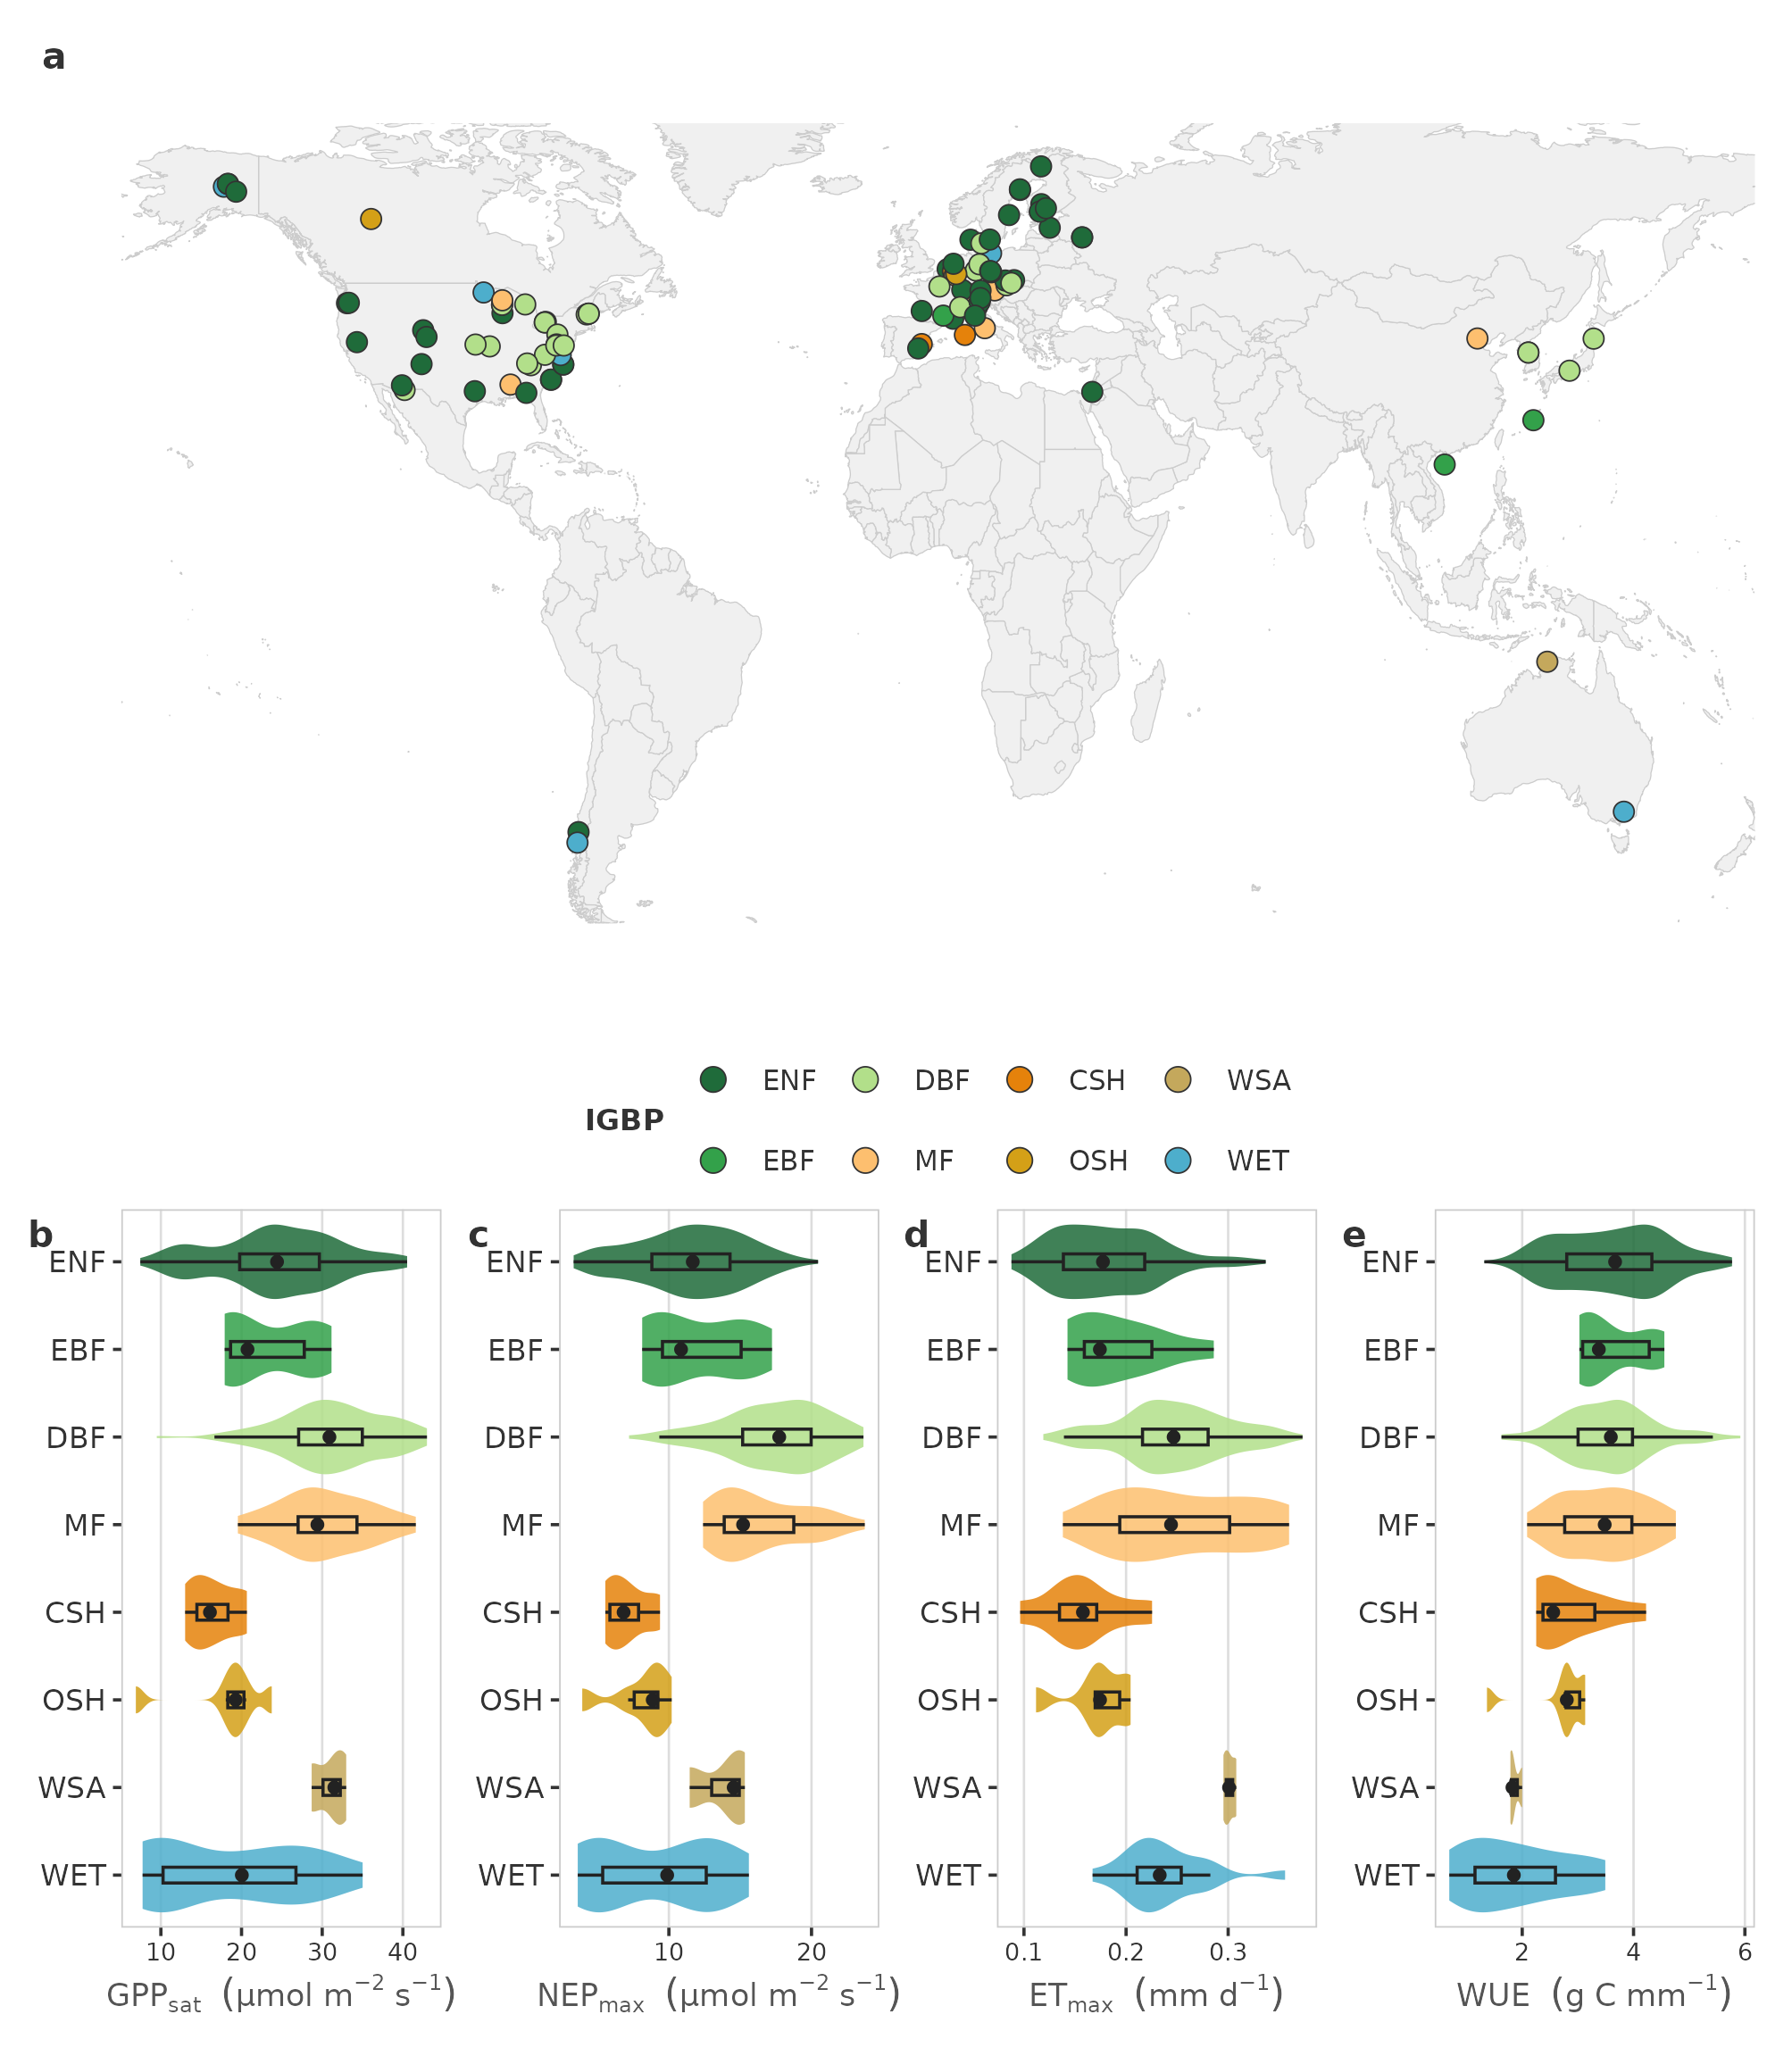
\includegraphics[width=\linewidth]{figures/fig1_site_map.png}\end{center}

\textbf{Model skill (AutoGluon)}
\begin{itemize}
  \item Repeated leave-one-site-out CV, $R^2$ of climate + traits (C+T) and climate + traits + mortality (C+T+M):
        adding mortality raises the mean $R^2$ from \textbf{0.349 to 0.402} (12\,months) and from \textbf{0.351 to 0.408}
        (24\,months) (Table~\ref{tab:r2}).
  \item Largest gain for NEP$_{max}$ (+0.11), then WUE (+0.06) and GPP$_{sat}$ (+0.04--0.05); ET$_{max}$ unchanged.
  \item Overall error change when mortality is added: MAE $-11.8$ / $-10.8$\,\% (NEP$_{max}$, 12 / 24\,m),
        $-4.1$ / $-5.7$\,\% (GPP$_{sat}$), $-4.3$ / $-4.7$\,\% (WUE), $-1.3$ / $-2.0$\,\% (ET$_{max}$).
  \item AutoGluon is slightly better than XGBoost and LightGBM on average (best in 7 of 16 tasks; Table~\ref{tab:a_r2}).
\end{itemize}

\begin{table}[htbp]
\centering
\caption{AutoGluon skill under repeated leave-one-site-out CV ($R^2$), without (C+T) and with mortality (C+T+M).}
\label{tab:r2}
\footnotesize
\begin{tabular}{lcccccc}
\toprule
 & \multicolumn{3}{c}{12 months} & \multicolumn{3}{c}{24 months} \\
\cmidrule(lr){2-4}\cmidrule(lr){5-7}
EFP & C+T & C+T+M & $\Delta$ & C+T & C+T+M & $\Delta$ \\
\midrule
GPP$_\mathrm{sat}$ & 0.330 & 0.367 & +0.037 & 0.317 & 0.370 & +0.053 \\
NEP$_\mathrm{max}$ & 0.391 & 0.503 & +0.112 & 0.394 & 0.502 & +0.108 \\
ET$_\mathrm{max}$  & 0.423 & 0.425 & +0.002 & 0.429 & 0.433 & +0.004 \\
WUE                & 0.252 & 0.312 & +0.060 & 0.264 & 0.326 & +0.062 \\
\midrule
Mean               & 0.349 & 0.402 & +0.053 & 0.351 & 0.408 & +0.057 \\
\bottomrule
\end{tabular}
\end{table}

\textbf{Figure 2 and Tables~\ref{tab:t1}--\ref{tab:t2}: Does mortality reduce the prediction error?}
\begin{itemize}
  \item \textbf{NEP$_{max}$: yes, robustly.} Mortality lowers the MAE by about 8--12\,\% across all sites and by
        17--32\,\% at high-mortality sites and years. Significant in all bootstrap columns at 12\,m and in all but
        the High-site column at 24\,m; in the log-ratio test significant at 12\,m only (24\,m: same direction, $-8$ to $-17$\,\%).
  \item \textbf{GPP$_{sat}$: smaller} ($-4$ to $-9$\,\%), significant at the Mid + High sites and at site level.
  \item \textbf{WUE: only where mortality happened.} Across all sites $\pm$0--5\,\%; at high-mortality sites and in
        high-mortality years $-11$ to $-22$\,\%, significant in the bootstrap (Table~\ref{tab:t2}).
  \item \textbf{ET$_{max}$: small} ($-1$ to $-6$\,\% across all sites, up to $-12$\,\% at High sites and in high-mortality
        years), significant only in a few 24\,m cells.
  \item \textbf{Table~\ref{tab:t1}} (site level): per-site MAE ratio, paired sign-flip permutation test on the log ratios.
        The log ratio stops sites with an almost perfect C+T prediction from dominating, which happened with the
        mean of per-site \% changes (one-year sites, e.g.\ +275\,\% at KR-Kw1 from a tiny absolute change).
  \item \textbf{Table~\ref{tab:t2}} (paired bootstrap): at the \textbf{site-year level} every year is its own
        observation, so years without mortality do not dilute the years with mortality. Whole sites are resampled and
        permuted, because the years of one site are not independent.
  \item \textbf{The effect is largest in the years when mortality happened:} NEP$_{max}$ MAE $-29$ to $-32$\,\% in
        high-mortality years vs $-11$ to $-12$\,\% over all site-years; WUE $-17$ to $-22$\,\% vs $-4$ to $-5$\,\%.
  \item The bootstrap intervals and the permutation tests agree: every significant cell has its 95\,\% interval
        entirely below zero.
  \item Robustness: the same picture with RMSE (Tables~\ref{tab:a1}, \ref{tab:a2}), with XGBoost and LightGBM
        (Tables~\ref{tab:a3}, \ref{tab:a4}), when weighting sites by their number of years, and when dropping the
        one-year sites. Keeping only sites with $\geq$3 years removes about a quarter of the High sites (22 $\rightarrow$ 16); NEP$_{max}$ still
        improves but fewer cells stay significant.
  \item Fig.~2 shows the per-site RMSE distributions with the median change and a paired Wilcoxon test (Wilcoxon asks
        whether most sites improve; it is more liberal than the permutation test).
  \item \decide{Fig.~2: switch to MAE and the permutation test, so the figure matches Tables~\ref{tab:t1}--\ref{tab:t2}?}
  \item \decide{main statistic: site-level log-ratio permutation (Table~\ref{tab:t1}) or site-year bootstrap (Table~\ref{tab:t2})?}
\end{itemize}

\begin{center}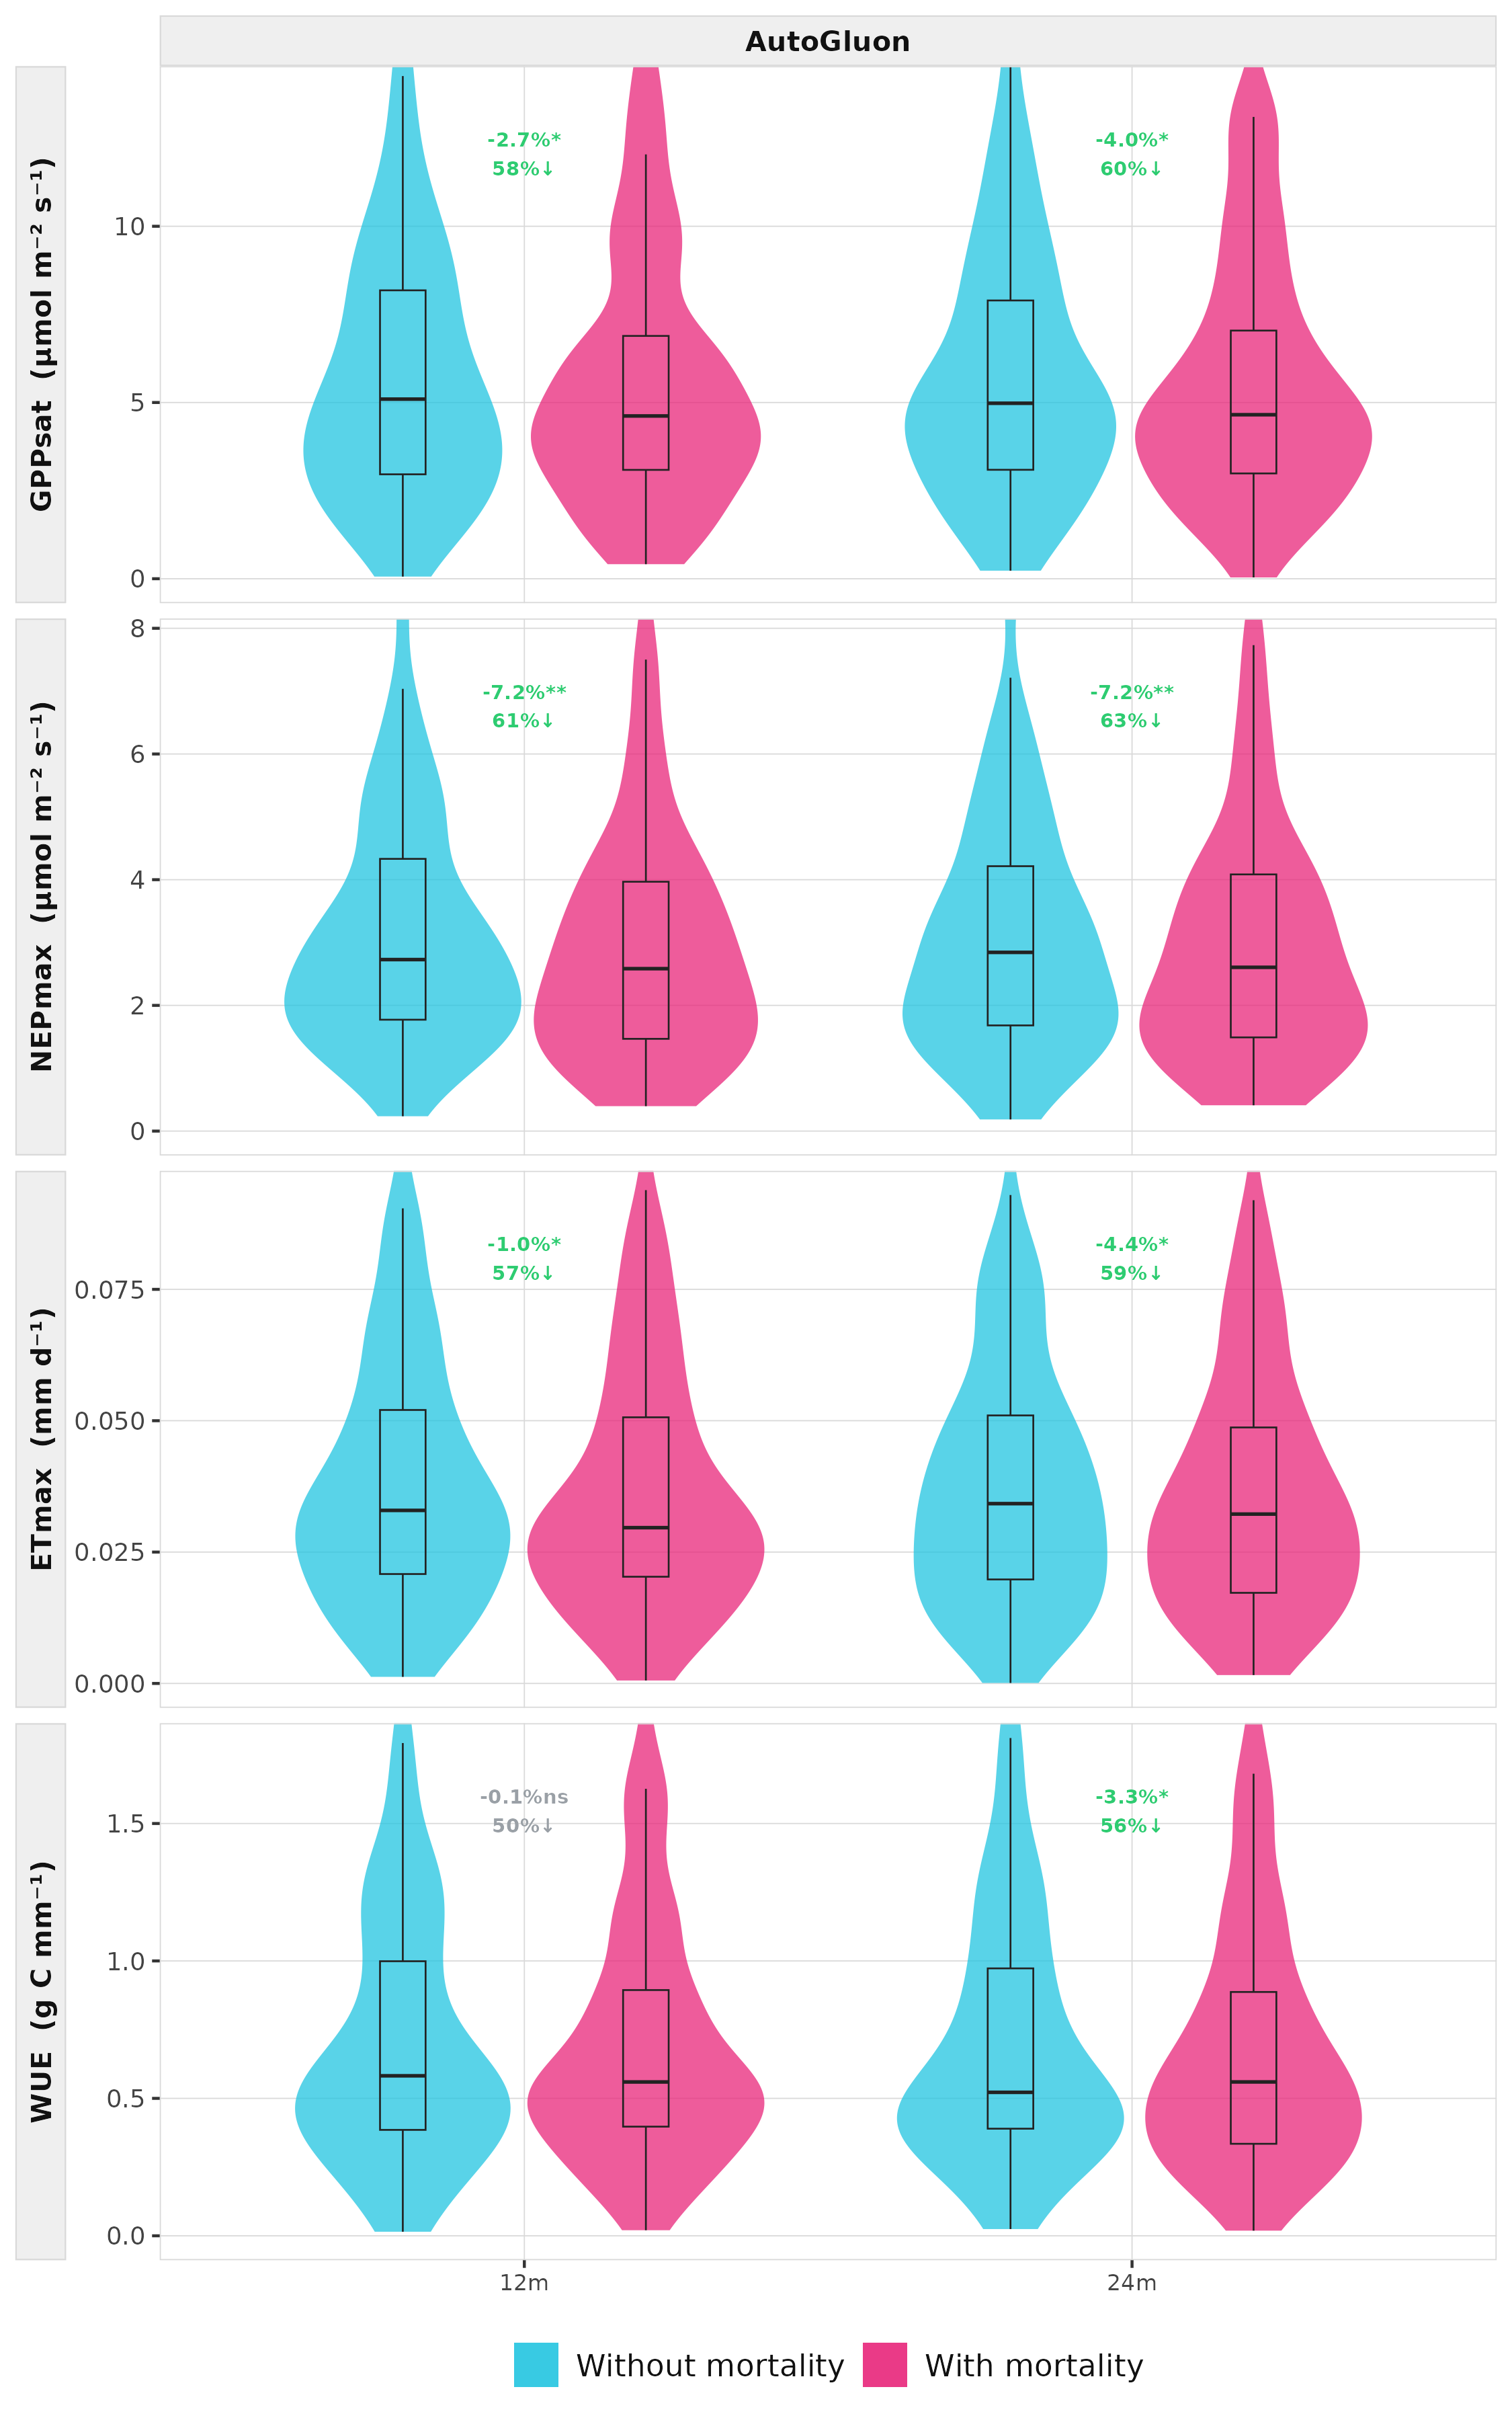
\includegraphics[width=0.62\linewidth]{figures/fig2_AG.png}\\[2pt]
{\small \textbf{Fig.\ 2a} --- per-site RMSE without (cyan) and with mortality (pink), AutoGluon, all 101 sites;
\% = median paired change, stars = one-sided paired Wilcoxon (BH-FDR), \%$\downarrow$ = share of sites improved.}\end{center}

\begin{center}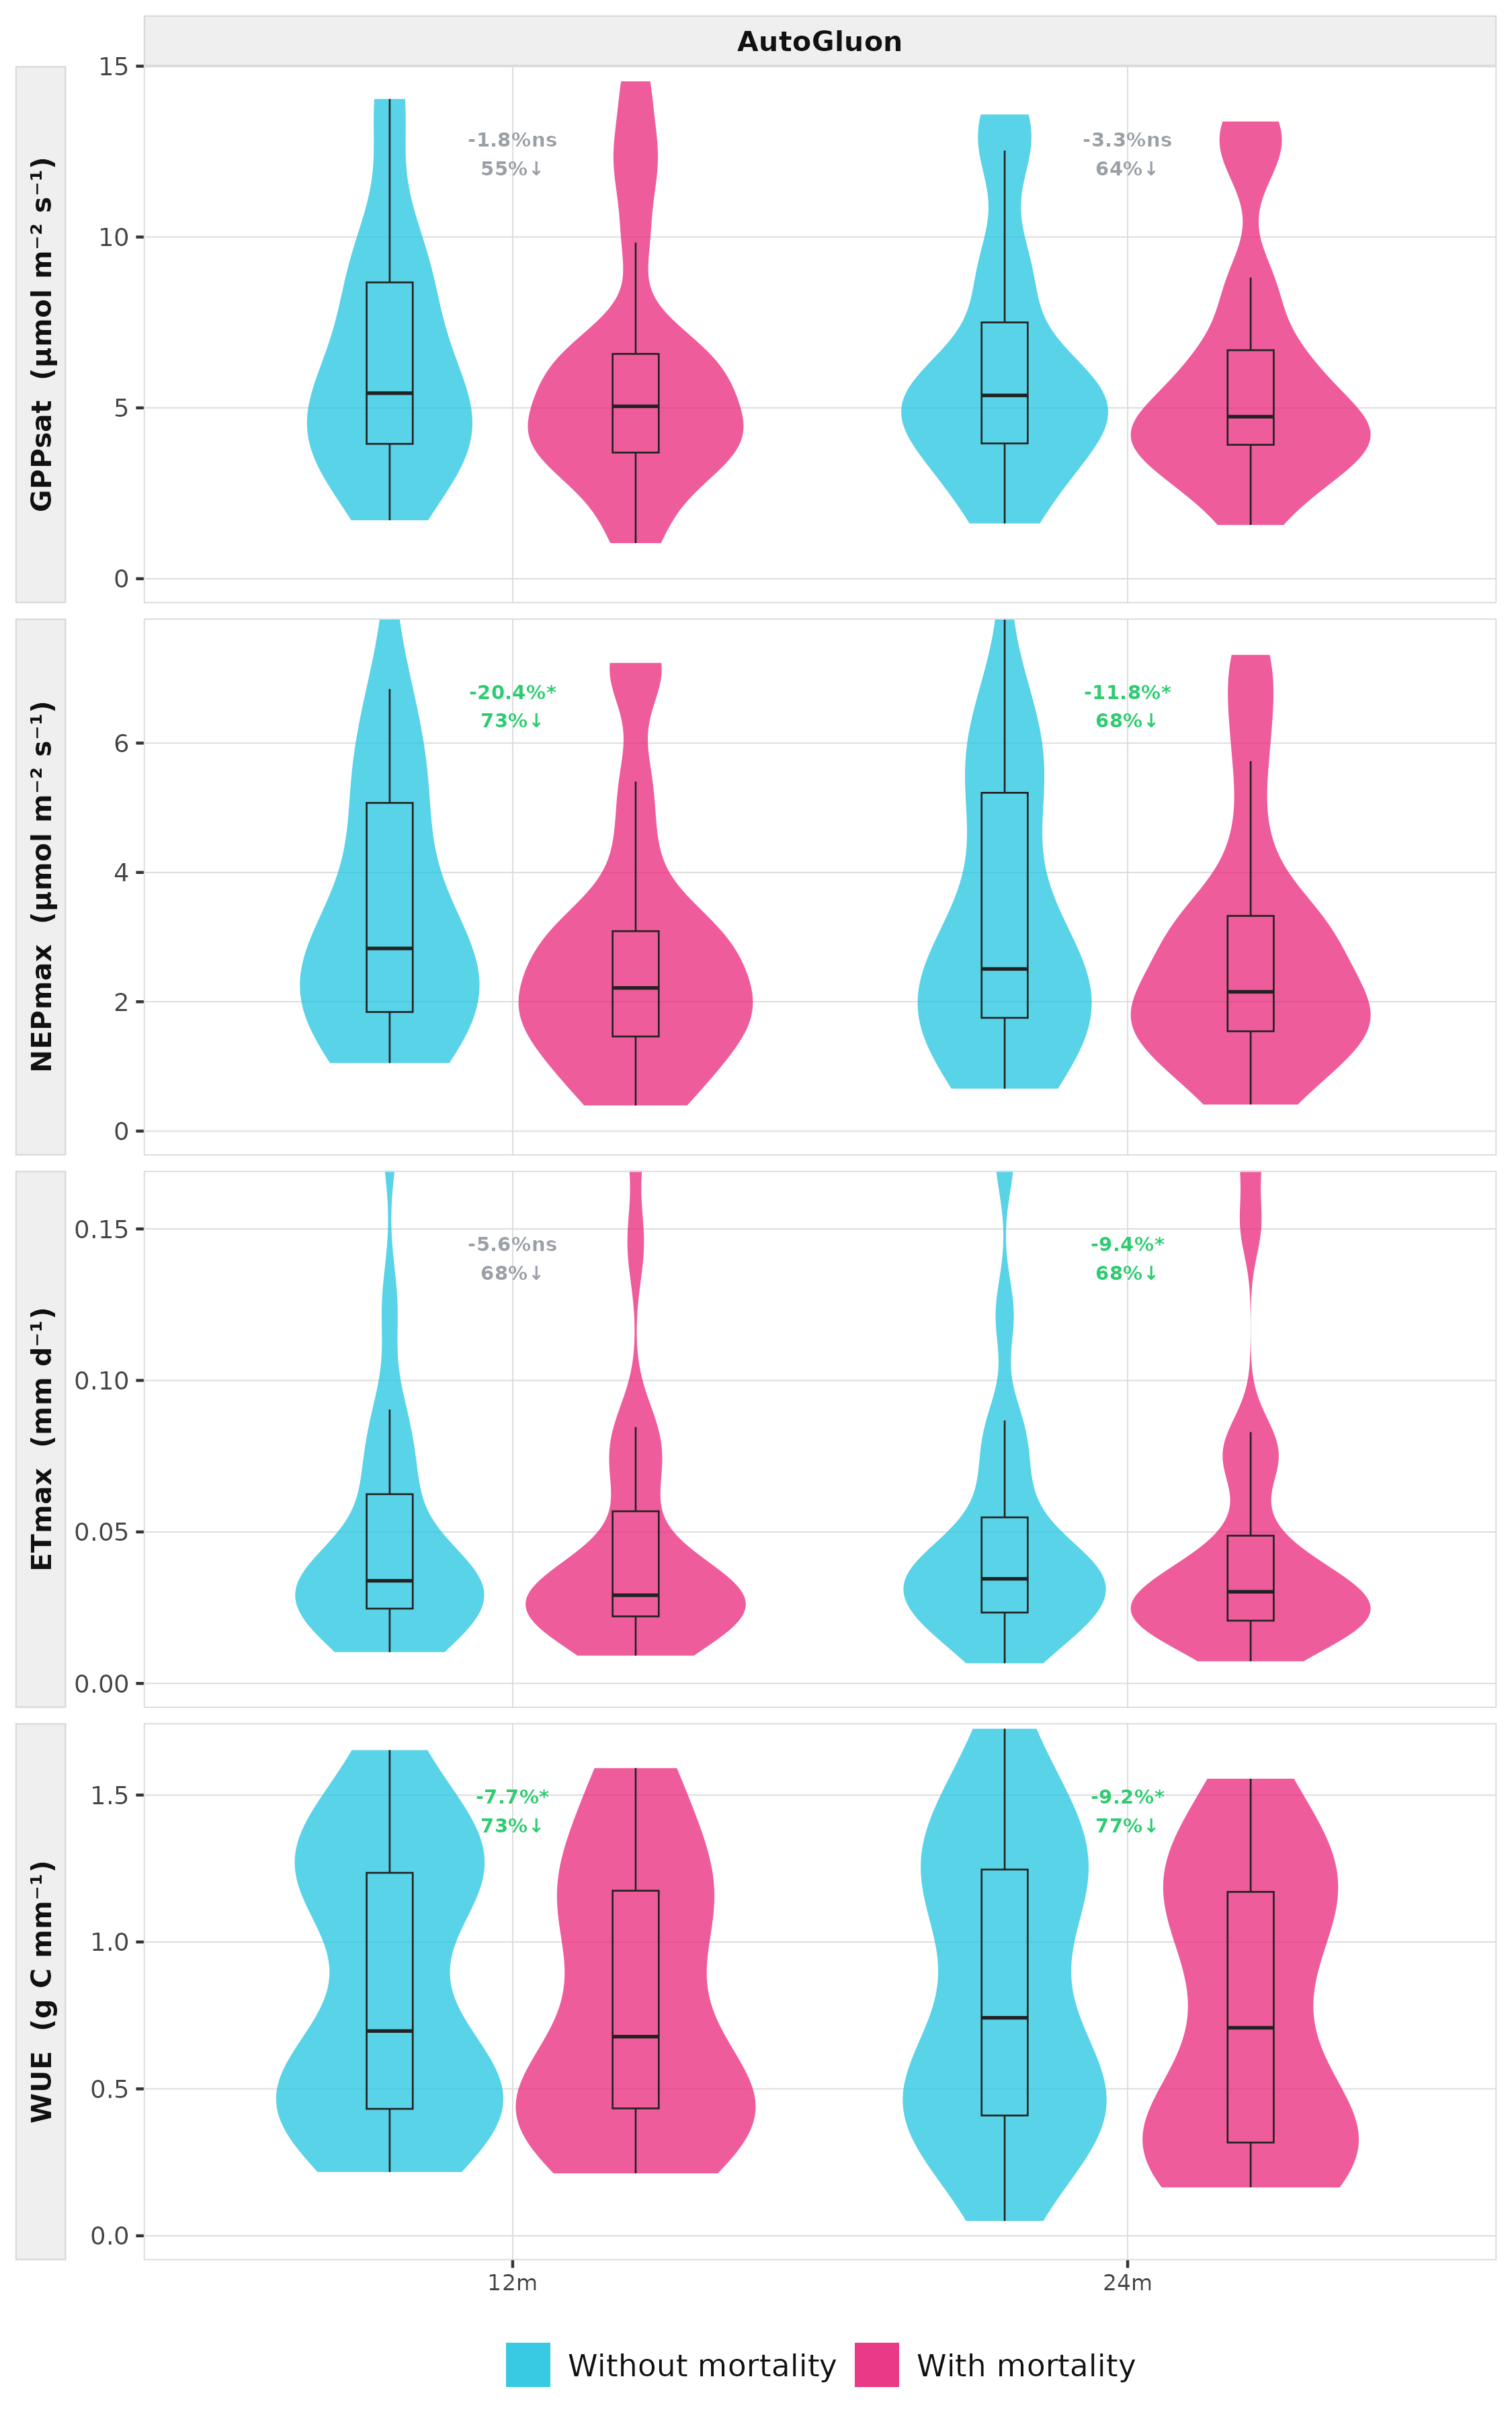
\includegraphics[width=0.62\linewidth]{figures/fig2b_high_AG.png}\\[2pt]
{\small \textbf{Fig.\ 2b} --- the same, high total-mortality sites only (22 sites; models trained on all sites).
NEP$_{max}$ $-20$ / $-12$\,\%, WUE $-8$ / $-9$\,\%, ET$_{max}$ $-6$ / $-9$\,\% (12 / 24\,m).}\end{center}

\begin{center}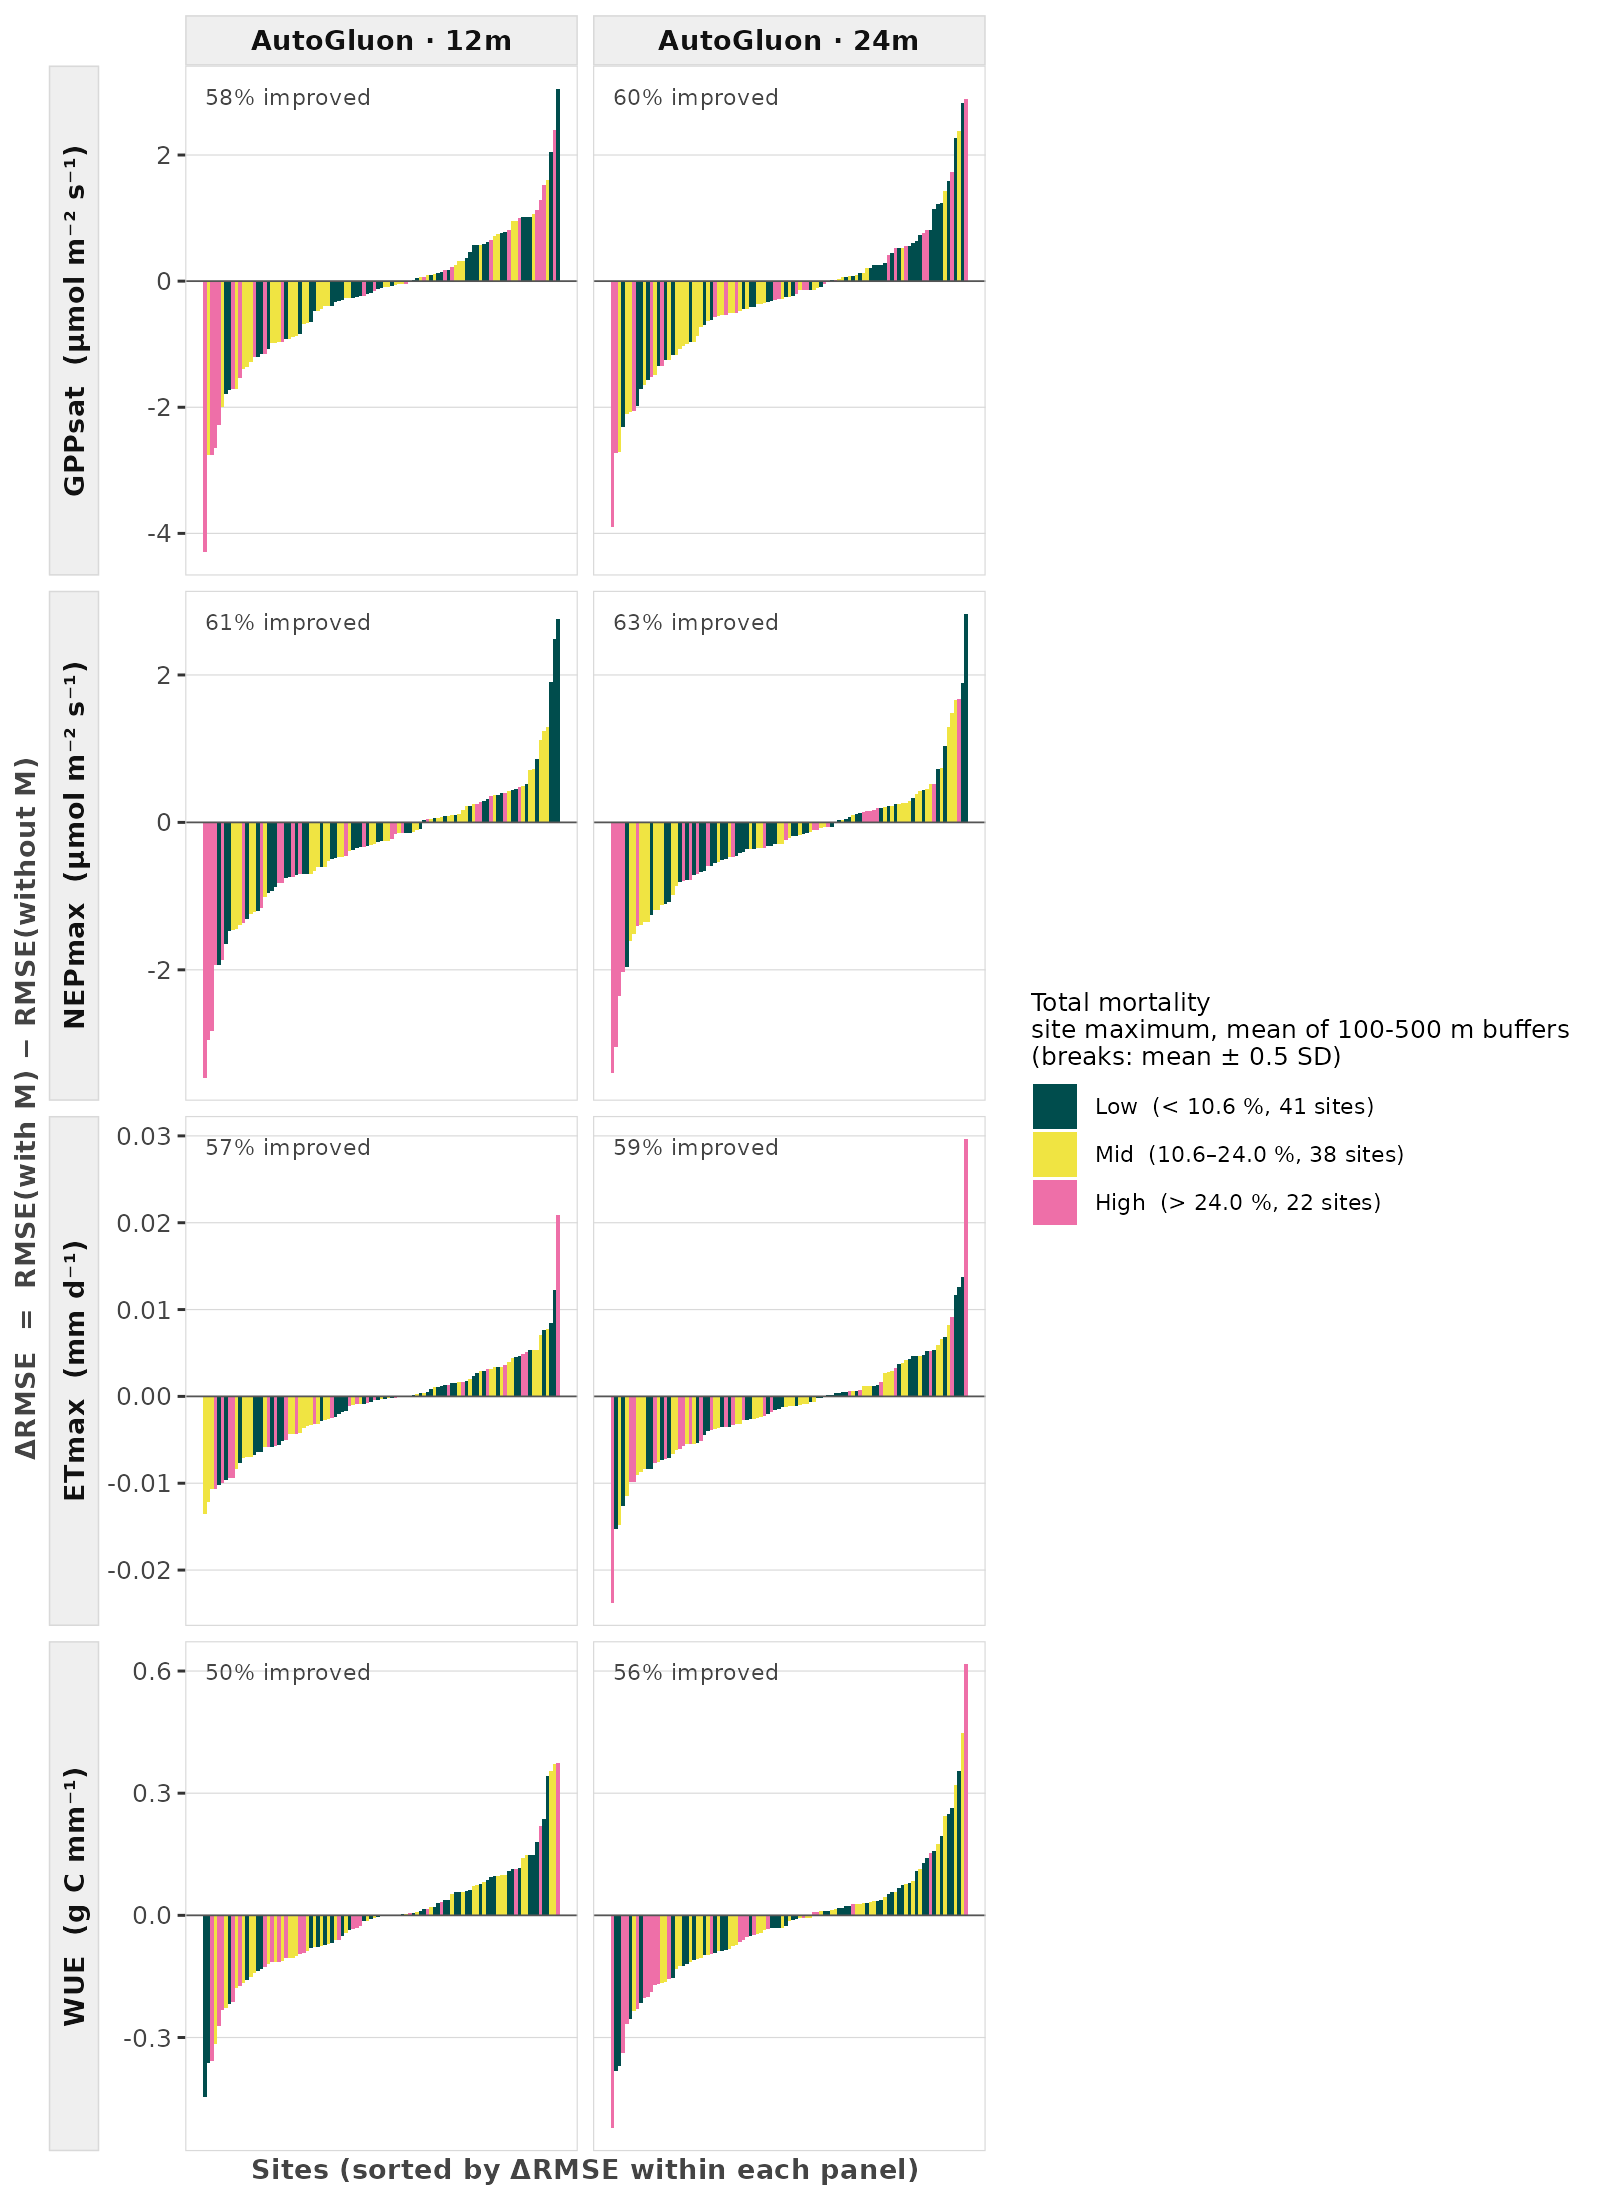
\includegraphics[width=0.7\linewidth]{figures/fig2c_site_dRMSE_AG.png}\\[2pt]
{\small \textbf{Fig.\ 2c} --- per-site $\Delta$RMSE, AutoGluon, bars coloured by total-mortality class.
The largest improvements are at High sites (pink) for GPP$_{sat}$ and NEP$_{max}$.}\end{center}

\begin{table}[htbp]
\centering
\caption{Effect of adding mortality predictors on per-site prediction error (summary of Fig.~2). For every site, MAE of the model with climate, traits and mortality (C+T+M) is compared with the model without mortality (C+T), both evaluated by repeated leave-one-site-out cross-validation (3 $\times$ 80\%). $\Delta$MAE = geometric mean over sites of the paired error ratio, (exp(mean$_\mathrm{sites}$ ln(MAE$_\mathrm{C+T+M}$ / MAE$_\mathrm{C+T}$)) $-$ 1) $\times$ 100; negative values mean that mortality reduces the error. Improved = share of sites whose MAE decreased. Sites are grouped by their maximum total mortality across years (averaged over the five buffers, 100--500\,m); High $>$ mean $+$ 0.5\,SD (24.0\%), Low $<$ mean $-$ 0.5\,SD (10.6\%), Mid in between. Stars: one-sided paired permutation test on the per-site log error ratios (100\,000 random sign flips; C+T+M $<$ C+T), Benjamini--Hochberg corrected across all 72 tests of the three learners ($^{*}$\,$q<0.05$, $^{**}$\,$q<0.01$, $^{***}$\,$q<0.001$). Tree cover $\geq$ 30\%, 101 sites, 361 site-years, deadtrees v5.}
\label{tab:t1}
\scriptsize
\setlength{\tabcolsep}{4pt}
\renewcommand{\arraystretch}{0.92}
\begin{tabular}{lllccc}
\toprule
Model & EFP & & All sites & Mid + High & High \\
 & & & ($n$ = 101) & ($n$ = 60) & ($n$ = 22) \\
\midrule
\multirow{8}{*}{\shortstack[l]{AutoGluon\\12\,months}} & \multirow{2}{*}{GPP$_\mathrm{sat}$} & $\Delta$MAE (\%) & $-3.9$ & $-8.6$$^{*}$ & $-12.4$ \\
 & & Improved (\%) & 59 & 62 & 59 \\
\cmidrule(l){2-6}
 & \multirow{2}{*}{NEP$_\mathrm{max}$} & $\Delta$MAE (\%) & $-12.2$$^{*}$ & $-14.5$$^{**}$ & $-29.8$$^{**}$ \\
 & & Improved (\%) & 63 & 62 & 77 \\
\cmidrule(l){2-6}
 & \multirow{2}{*}{ET$_\mathrm{max}$} & $\Delta$MAE (\%) & $-4.5$ & $-5.6$ & $-6.2$ \\
 & & Improved (\%) & 52 & 58 & 68 \\
\cmidrule(l){2-6}
 & \multirow{2}{*}{WUE} & $\Delta$MAE (\%) & $+1.4$ & $-5.2$ & $-11.0$ \\
 & & Improved (\%) & 52 & 60 & 73 \\
\midrule
\multirow{8}{*}{\shortstack[l]{AutoGluon\\24\,months}} & \multirow{2}{*}{GPP$_\mathrm{sat}$} & $\Delta$MAE (\%) & $-6.0$ & $-9.0$$^{**}$ & $-7.2$ \\
 & & Improved (\%) & 61 & 72 & 59 \\
\cmidrule(l){2-6}
 & \multirow{2}{*}{NEP$_\mathrm{max}$} & $\Delta$MAE (\%) & $-8.0$ & $-9.1$ & $-17.4$ \\
 & & Improved (\%) & 62 & 57 & 64 \\
\cmidrule(l){2-6}
 & \multirow{2}{*}{ET$_\mathrm{max}$} & $\Delta$MAE (\%) & $-3.6$ & $-6.9$$^{*}$ & $-12.3$ \\
 & & Improved (\%) & 64 & 72 & 73 \\
\cmidrule(l){2-6}
 & \multirow{2}{*}{WUE} & $\Delta$MAE (\%) & $-2.1$ & $-6.1$ & $-15.4$ \\
 & & Improved (\%) & 56 & 63 & 77 \\
\bottomrule
\end{tabular}
\end{table}

\begin{table}[htbp]
\centering
\caption{Paired bootstrap of the change in MAE when mortality is added (C+T $\rightarrow$ C+T+M), AutoGluon. Cells: \% change of the error, 100\,(MAE$_\mathrm{C+T+M}$ / MAE$_\mathrm{C+T}$ $-$ 1), with the 95\,\% bootstrap interval in brackets. \emph{Site level}: one MAE per site and model over its years, ratio of the mean site errors. \emph{Site-year level}: every site-year is an observation (pooled MAE; no averaging over years). Years of one site are not independent, so at both levels whole sites are resampled (10\,000 bootstrap draws) and the C+T / C+T+M labels are swapped per site for the paired permutation test (10\,000 draws, one-sided; stars, Benjamini--Hochberg corrected across all three learners: $^{*}$\,$q<0.05$, $^{**}$\,$q<0.01$, $^{***}$\,$q<0.001$). High sites: site maximum of total mortality $>$ 24.0\,\%; the last two columns keep only the site-years whose own total mortality exceeds 10.6\,\% (Mid + High) or 24.0\,\% (High). Column heads: sites / site-years. 101 sites, 361 site-years, deadtrees v5.}
\label{tab:t2}
\scriptsize
\setlength{\tabcolsep}{3pt}
\resizebox{\linewidth}{!}{%
\begin{tabular}{llccccc}
\toprule
 & & Site level & \multicolumn{4}{c}{Site-year level} \\
\cmidrule(lr){3-3}\cmidrule(lr){4-7}
 & & All sites & All sites & High sites & Mid + High years & High years \\
 & & (101 sites) & (101 / 361) & (22 / 80) & (60 / 160) & (22 / 40) \\
\midrule
\multirow{4}{*}{\shortstack[l]{AutoGluon\\12\,months}} & GPP$_\mathrm{sat}$ & $-4.6$ {\tiny[$-8.6$, $-0.5$]}$^{*}$ & $-4.1$ {\tiny[$-8.0$, $-0.2$]} & $-7.2$ {\tiny[$-18.1$, $+2.9$]} & $-6.7$ {\tiny[$-12.8$, $-0.7$]}$^{*}$ & $-12.0$ {\tiny[$-29.5$, $+4.9$]} \\
 & NEP$_\mathrm{max}$ & $-10.1$ {\tiny[$-15.5$, $-4.4$]}$^{**}$ & $-11.8$ {\tiny[$-17.0$, $-6.3$]}$^{**}$ & $-22.6$ {\tiny[$-33.6$, $-11.1$]}$^{**}$ & $-12.5$ {\tiny[$-20.1$, $-4.9$]}$^{*}$ & $-31.6$ {\tiny[$-43.2$, $-16.0$]}$^{*}$ \\
 & ET$_\mathrm{max}$ & $-2.5$ {\tiny[$-5.6$, $+0.5$]} & $-1.3$ {\tiny[$-4.2$, $+1.3$]} & $-2.9$ {\tiny[$-8.4$, $+2.1$]} & $-3.9$ {\tiny[$-7.7$, $+0.0$]} & $-9.7$ {\tiny[$-20.6$, $+2.7$]} \\
 & WUE & $-3.2$ {\tiny[$-7.3$, $+1.3$]} & $-4.3$ {\tiny[$-8.1$, $-0.2$]} & $-10.9$ {\tiny[$-17.8$, $-4.3$]}$^{*}$ & $-7.2$ {\tiny[$-12.2$, $-1.8$]}$^{*}$ & $-16.9$ {\tiny[$-25.2$, $-5.1$]}$^{*}$ \\
\midrule
\multirow{4}{*}{\shortstack[l]{AutoGluon\\24\,months}} & GPP$_\mathrm{sat}$ & $-5.5$ {\tiny[$-9.4$, $-1.4$]}$^{*}$ & $-5.7$ {\tiny[$-9.5$, $-1.7$]}$^{*}$ & $-7.1$ {\tiny[$-17.2$, $+3.6$]} & $-8.3$ {\tiny[$-14.2$, $-2.6$]}$^{*}$ & $-11.1$ {\tiny[$-28.0$, $+8.1$]} \\
 & NEP$_\mathrm{max}$ & $-9.3$ {\tiny[$-14.4$, $-3.7$]}$^{**}$ & $-10.8$ {\tiny[$-16.0$, $-5.1$]}$^{**}$ & $-17.5$ {\tiny[$-30.7$, $-2.1$]} & $-11.6$ {\tiny[$-19.8$, $-2.7$]}$^{*}$ & $-29.2$ {\tiny[$-42.9$, $-8.6$]}$^{*}$ \\
 & ET$_\mathrm{max}$ & $-3.8$ {\tiny[$-7.3$, $-0.1$]}$^{*}$ & $-2.0$ {\tiny[$-5.0$, $+0.9$]} & $-5.3$ {\tiny[$-13.1$, $+1.2$]} & $-5.4$ {\tiny[$-9.6$, $-1.3$]}$^{*}$ & $-11.4$ {\tiny[$-23.7$, $+3.2$]} \\
 & WUE & $-3.6$ {\tiny[$-8.3$, $+1.6$]} & $-4.7$ {\tiny[$-9.1$, $-0.1$]} & $-14.8$ {\tiny[$-23.9$, $-6.4$]}$^{*}$ & $-8.2$ {\tiny[$-14.5$, $-1.5$]}$^{*}$ & $-21.8$ {\tiny[$-34.5$, $-8.2$]}$^{*}$ \\
\bottomrule
\end{tabular}}
\end{table}


\clearpage
\section*{Figure 3: Direction of the mortality effect at each site (signed SHAP)}
\begin{itemize}
  \item C+T+M model, per site the \textbf{net signed SHAP of the mortality block} (sum over the mortality predictors,
        averaged over the site's years, response units). Sites sorted by their maximum \textbf{total mortality} (mean
        of the five buffers), highest on the left; dashed lines = Low / Mid / High breaks (10.6\,\% and 24.0\,\%).
        Below zero = the model predicts a \emph{lower} EFP at that site because of its mortality values.
  \item AutoGluon, 24-month window; the 12-month window and XGBoost / LightGBM are in the Appendix.
  \item \textbf{The sign follows the mortality class.} Share of sites with a negative contribution (24\,m), Low / Mid / High:
        GPP$_{sat}$ 7 / 66 / 86\,\%; NEP$_{max}$ 10 / 68 / 91\,\%; WUE 2 / 58 / 86\,\%; ET$_{max}$ 24 / 50 / 77\,\%.
        The 12-month window gives the same picture.
  \item \textbf{Size:} median $-2.1$ (GPP$_{sat}$) and $-1.5$ (NEP$_{max}$) $\mu$mol\,m$^{-2}$\,s$^{-1}$ at High
        sites, $+1.4$ and $+1.2$ at Low sites; ET$_{max}$ contributions are tiny ($\pm$0.005\,mm\,d$^{-1}$).
  \item Overall importance (share of mean $|$SHAP$|$, C+T+M): mortality 24\,\% (GPP$_{sat}$), 28\,\% (NEP$_{max}$),
        16\,\% (ET$_{max}$), 23\,\% (WUE); climate 52--66\,\%; traits 11--20\,\%.
\end{itemize}

\begin{sidewaysfigure}
\centering
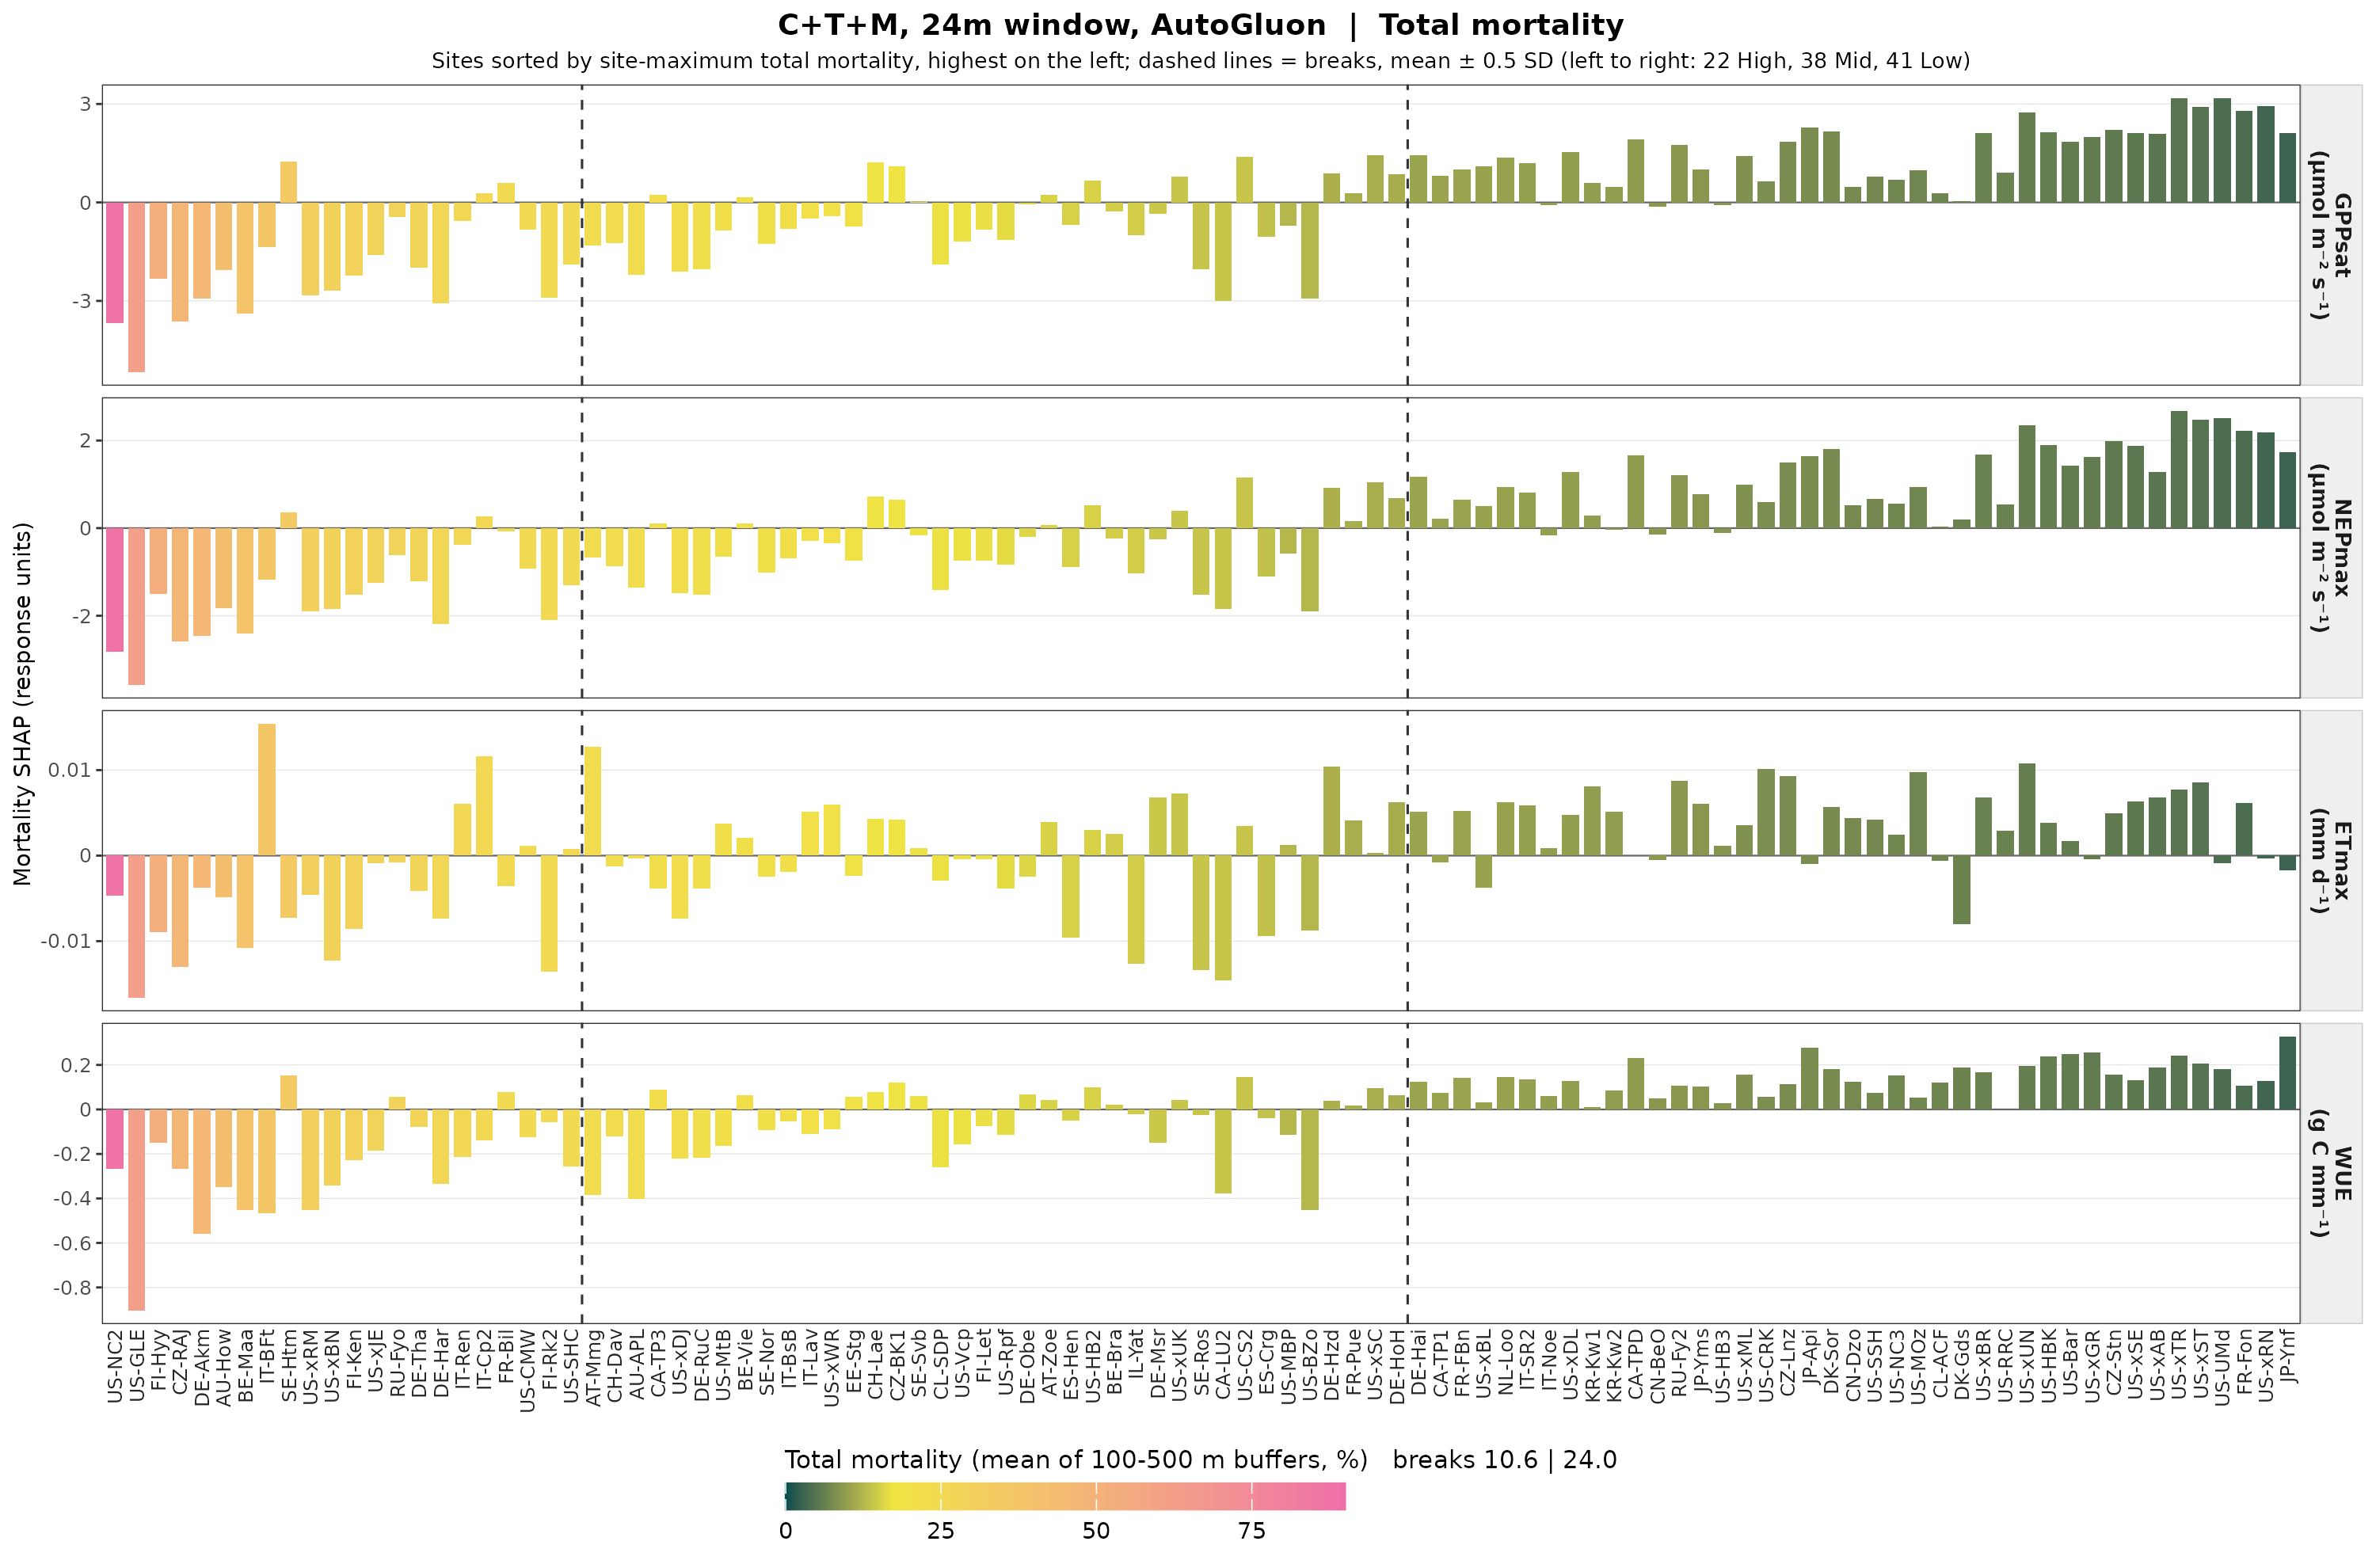
\includegraphics[width=\linewidth]{figures/fig3_signed_24m_AG.png}\\[2pt]
{\small \textbf{Fig.\ 3} --- Net signed mortality SHAP per site, C+T+M model, 24\,m, AutoGluon; sites sorted and
coloured by total mortality (mean of the five buffers).}
\end{sidewaysfigure}

\textbf{Figure 4: Does the direction differ between High and Low+Mid sites?} (signed SHAP)
\begin{itemize}
  \item Per site-year we sum the signed SHAP across the mortality predictors --- the block's net push on the
        prediction, in response units --- and average over the site's years. \textbf{Below zero means the model
        predicts a LOWER value of the EFP} (not that it predicts less accurately). Accuracy is Figure 2.
  \item Classes: site maximum of total mortality (mean of the five buffers); High $>$ mean + 0.5\,SD (22 High vs 79
        Low+Mid). Mann--Whitney U between the two groups, BH-FDR across the figure.
  \item \textbf{A clear dose--response.} At \textbf{High}-mortality sites the block pushes predicted carbon uptake
        \emph{down}; at \textbf{Low+Mid} sites slightly \emph{up} (relative to the average site).
  \item GPP$_{sat}$: High $-1.83$ / $-2.15$, Low+Mid $+0.47$ / $+0.66$ $\mu$mol\,m$^{-2}$\,s$^{-1}$ (12 / 24\,m);
        NEP$_{max}$: High $-1.61$ / $-1.51$, Low+Mid $+0.37$ / $+0.51$; WUE: High $-0.22$ / $-0.24$, Low+Mid
        $+0.07$ g\,C\,mm$^{-1}$; ET$_{max}$: tiny ($-0.003$ / $-0.005$\,mm\,d$^{-1}$). All 8 tests $q<0.001$.
  \item Split by relative deadwood instead (Appendix): the same for GPP$_{sat}$, NEP$_{max}$ and WUE; ET$_{max}$ not significant.
  \item \textbf{Read with Figure 2:} mortality improves accuracy by lowering predictions at damaged sites. Sites are
        grouped by the same variables whose contribution is measured, so the test confirms that the learned
        relationship is consistent; the direction and size are the informative part.
\end{itemize}

\begin{center}
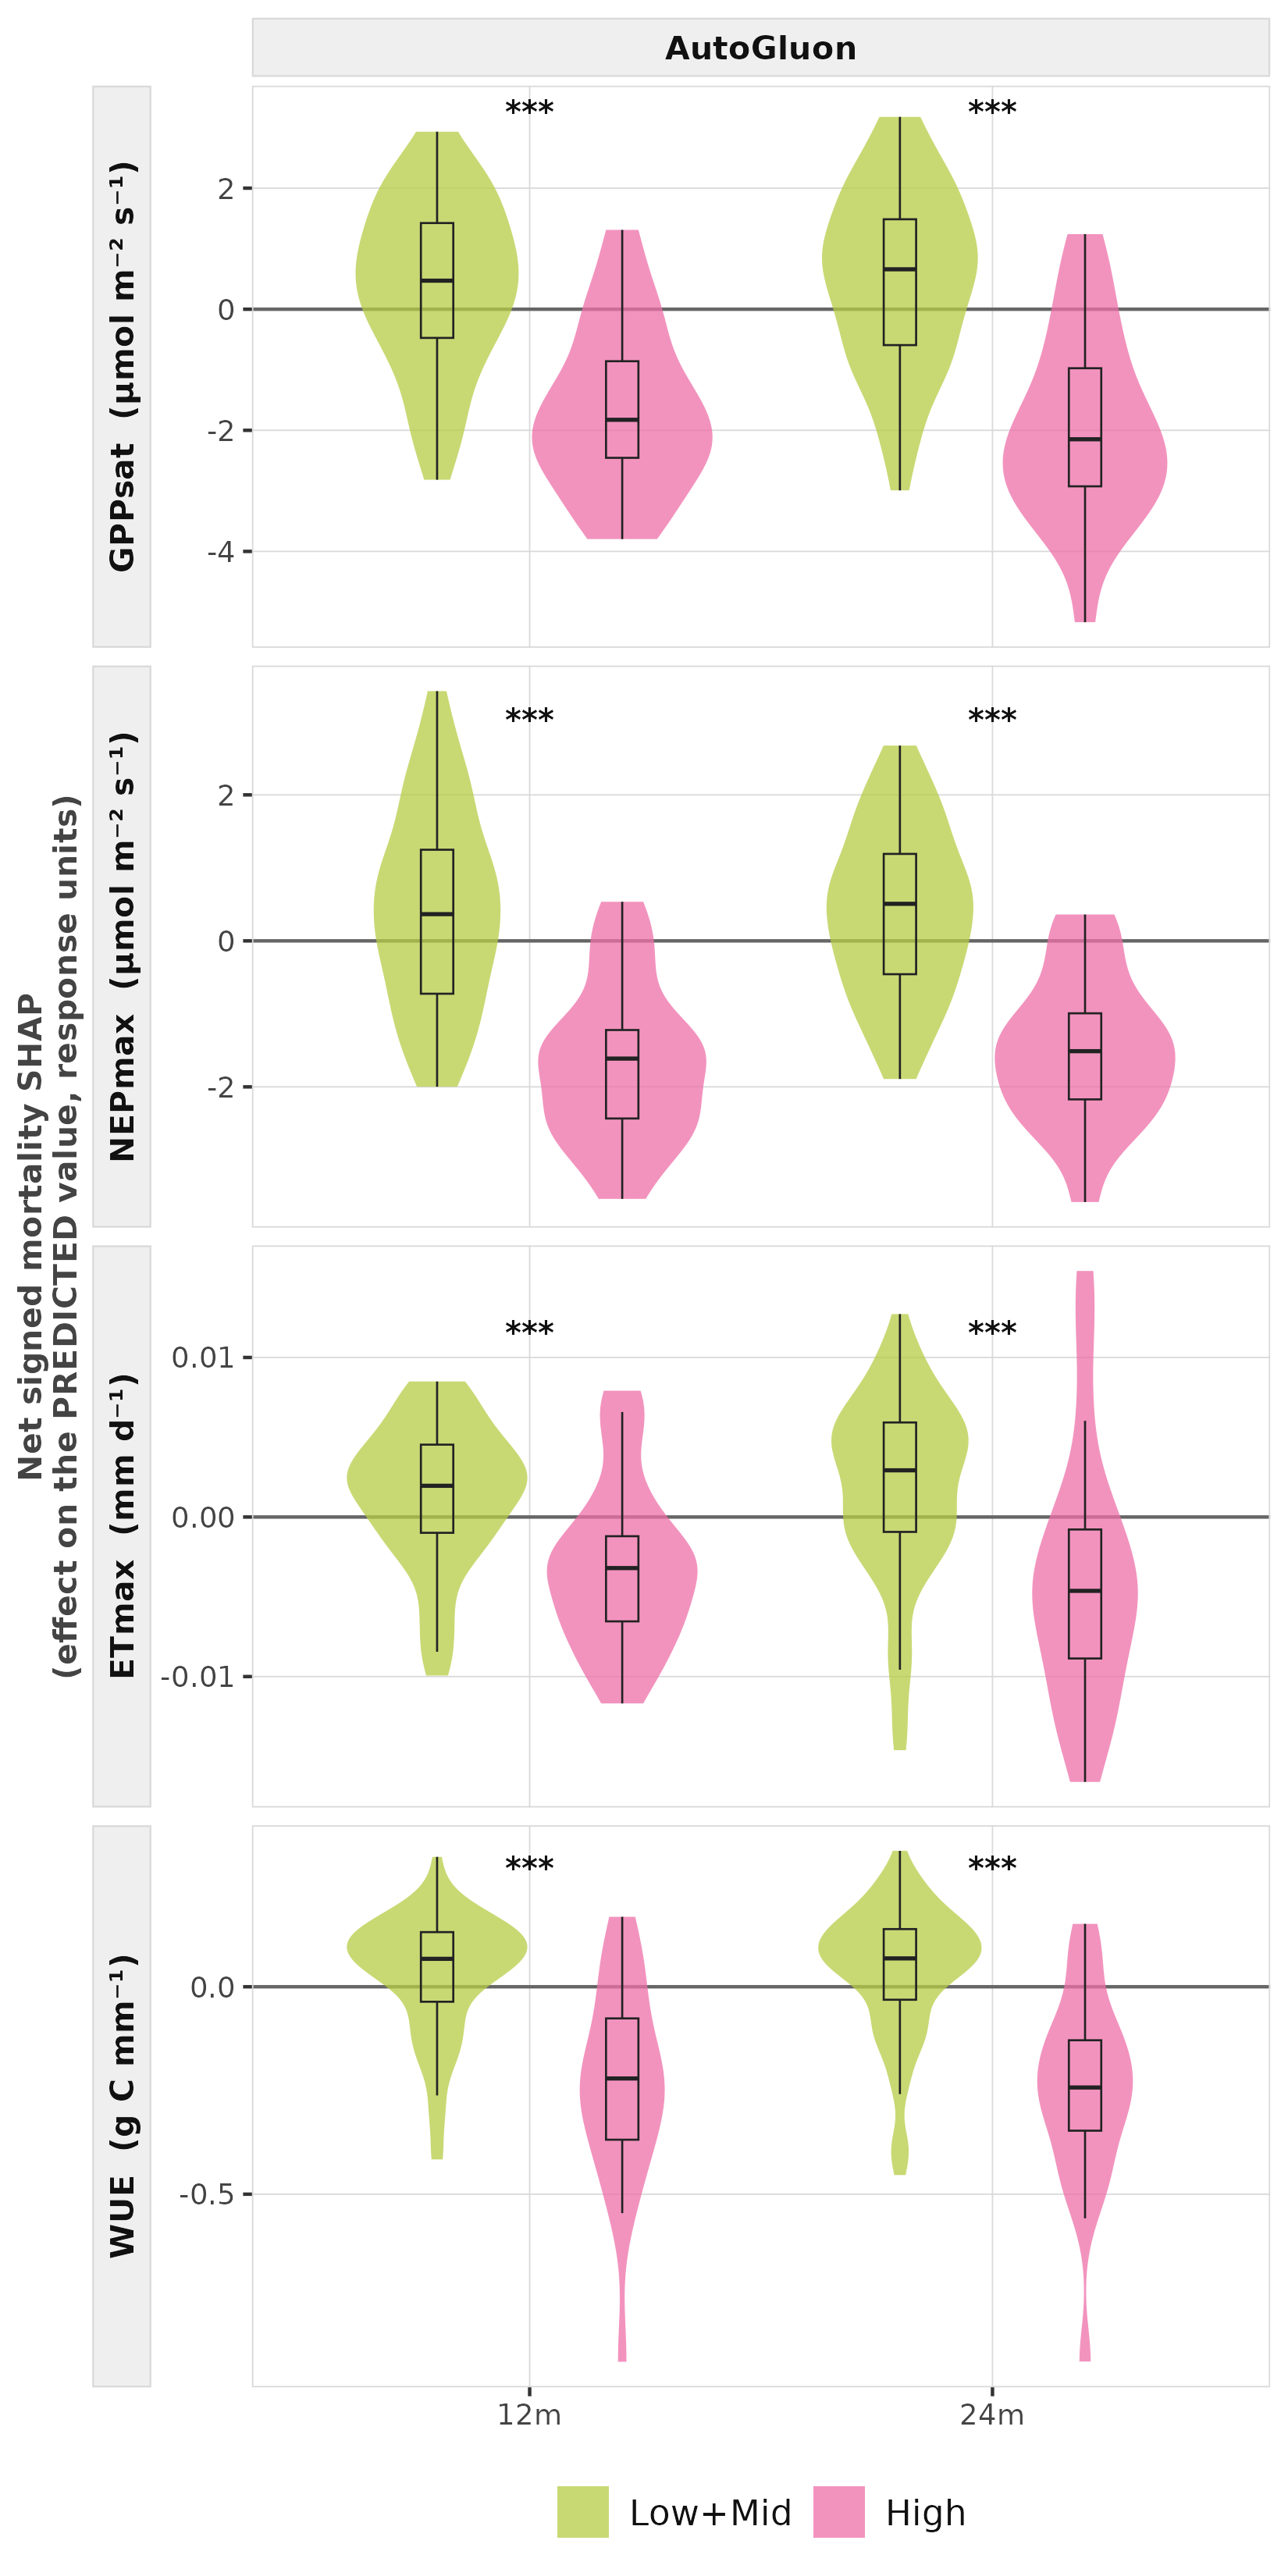
\includegraphics[width=0.48\linewidth]{figures/fig4_total_mort_AG.png}\\[2pt]
{\small \textbf{Fig.\ 4} --- net signed mortality SHAP, Low+Mid vs High total-mortality sites, AutoGluon.}
\end{center}

\textbf{Figure 5: Does it depend on ecosystem type or tree cover?}
\begin{itemize}
  \item AutoGluon, C+T+M model, 24\,months. \textbf{A} $\Delta$RMSE by IGBP, \textbf{B} net signed mortality SHAP by
        IGBP, \textbf{C} tree cover vs benefit, \textbf{D} tree cover vs direction, \textbf{E} total mortality vs
        direction. C/D/E: linear fit with a Spearman test per panel, BH-FDR across the board.
  \item \textbf{Panel C (benefit):} no relationship with tree cover ($\rho$ = 0.10--0.18, n.s.).
  \item \textbf{Panel D (direction vs tree cover):} strong and positive, $\rho$ = +0.66 to +0.75, all $p<0.001$ ---
        at low tree cover mortality pulls predicted carbon uptake \emph{down}, at high tree cover it pushes it \emph{up}.
  \item \textbf{Panel E (direction vs mortality):} stronger still and negative, $\rho$ = $-0.81$ (GPP$_{sat}$),
        $-0.83$ (NEP$_{max}$), $-0.78$ (WUE), $-0.47$ (ET$_{max}$), all $p<0.001$.
  \item \textbf{Panel B:} DBF, EBF and MF mostly positive, CSH, OSH and WET negative, ENF slightly negative.
  \item \textbf{So:} the \emph{magnitude} of the benefit does not depend on tree cover or ecosystem type; the
        \emph{direction} does, and it tracks mortality more closely than vegetation class.
  \item \textbf{Caveats.} OSH has 2 sites, WSA 1, CSH and EBF 3 each, WET 6; the correlations use all 101 sites.
  \item \decide{drop the IGBP classes with $\leq$3 sites from panels A and B, or keep them with a caveat?}
\end{itemize}

\begin{center}
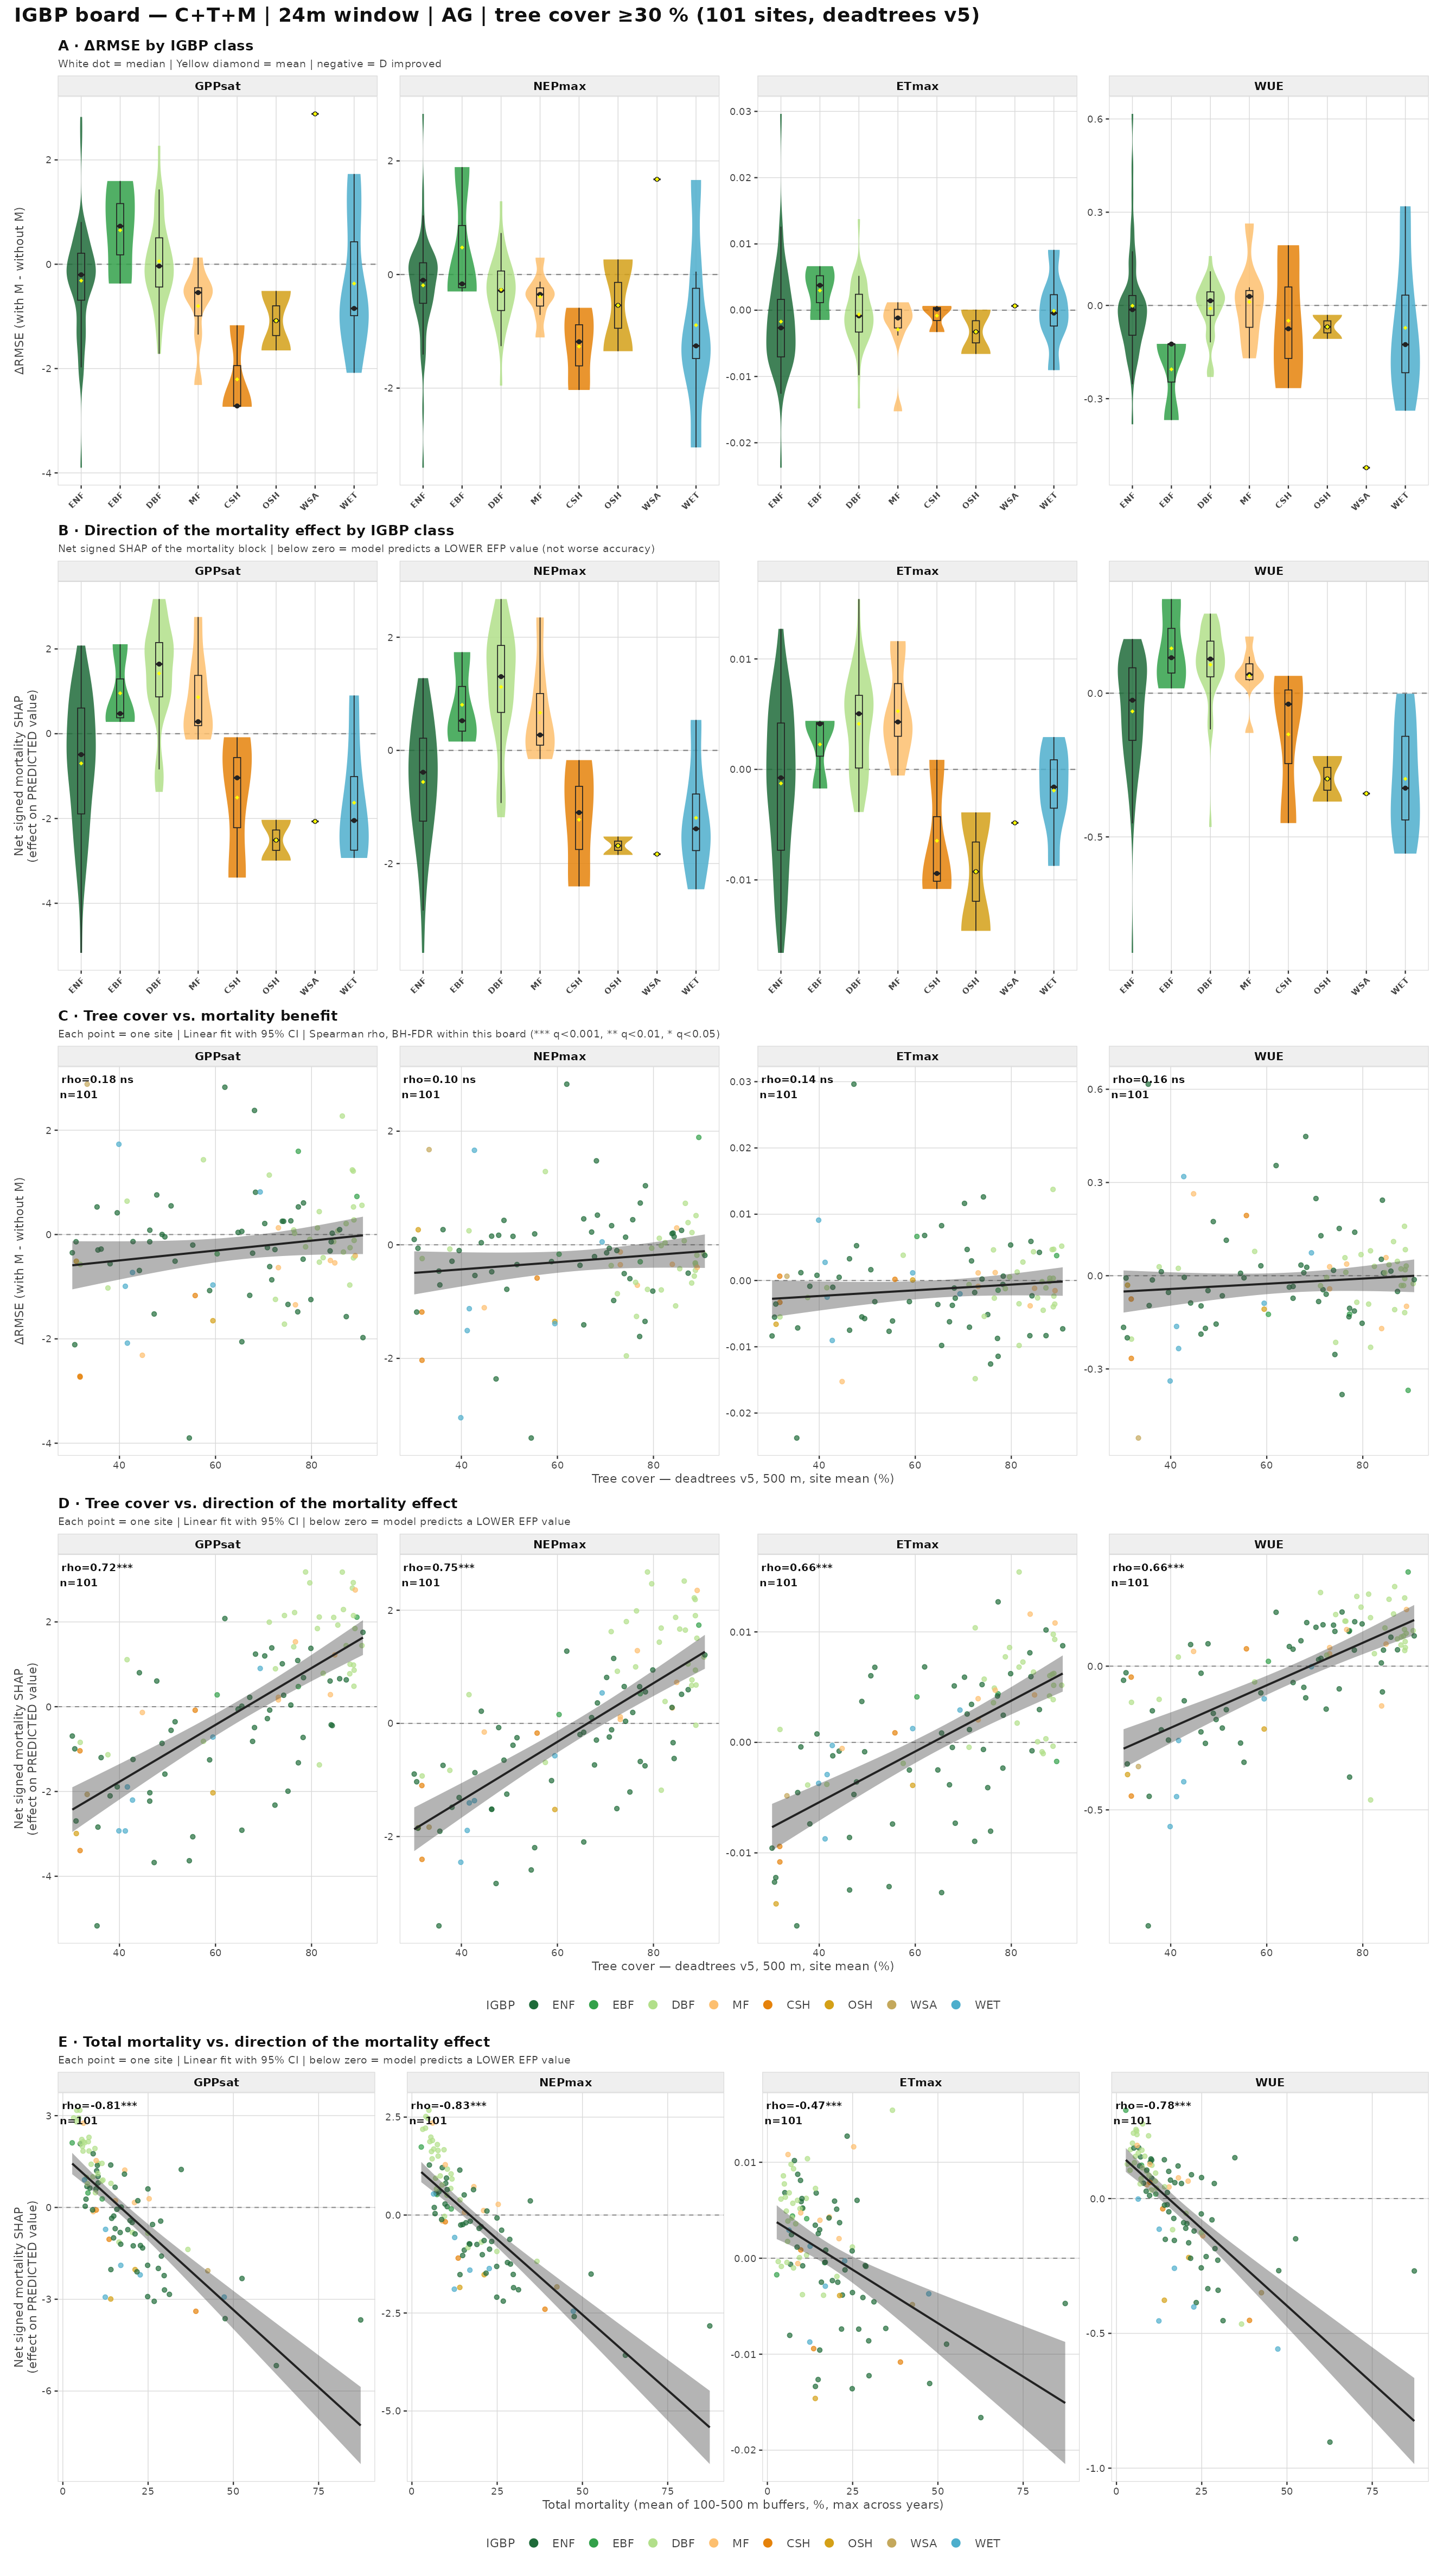
\includegraphics[width=0.82\linewidth]{figures/fig5_igbp_24m_AG.png}\\[2pt]
{\small \textbf{Fig.\ 5} --- AutoGluon, C+T+M model, 24\,m window (12\,m in the Appendix).}
\end{center}

\textbf{Figure 6: Which mortality metrics does the model use?}
\begin{itemize}
  \item Share of the mortality block's mean $|$SHAP$|$ per metric (C+T+M, mean over sites). AutoGluon:
        total mortality 26\,\%, relative deadwood 24\,\%, relative tree-cover loss 22\,\%, absolute deadwood 16\,\%,
        deadwood gain 12\,\%. For ET$_{max}$ tree-cover loss leads (32\,\%).
  \item \textbf{The metrics are largely interchangeable.} Drop-column test (XGBoost and LightGBM retrained without
        each metric, Appendix Fig.~A9): removing any single metric changes the error by at most about 1\,\%, because the
        correlated metrics take over (total mortality vs relative deadwood $\rho$ = 0.91).
  \item \textbf{Total mortality alone carries most of the effect:} added alone to C+T it gives 6.7--7.1\,\% of the
        7.6--8.9\,\% NEP$_{max}$ error reduction of the full block.
  \item Absolute deadwood gets 14--16\,\% of the SHAP but adds nothing when removed (credit borrowed from correlated metrics).
  \item \decide{reduce the mortality block to total mortality (+ relative deadwood) for a simpler model?}
\end{itemize}

\begin{center}
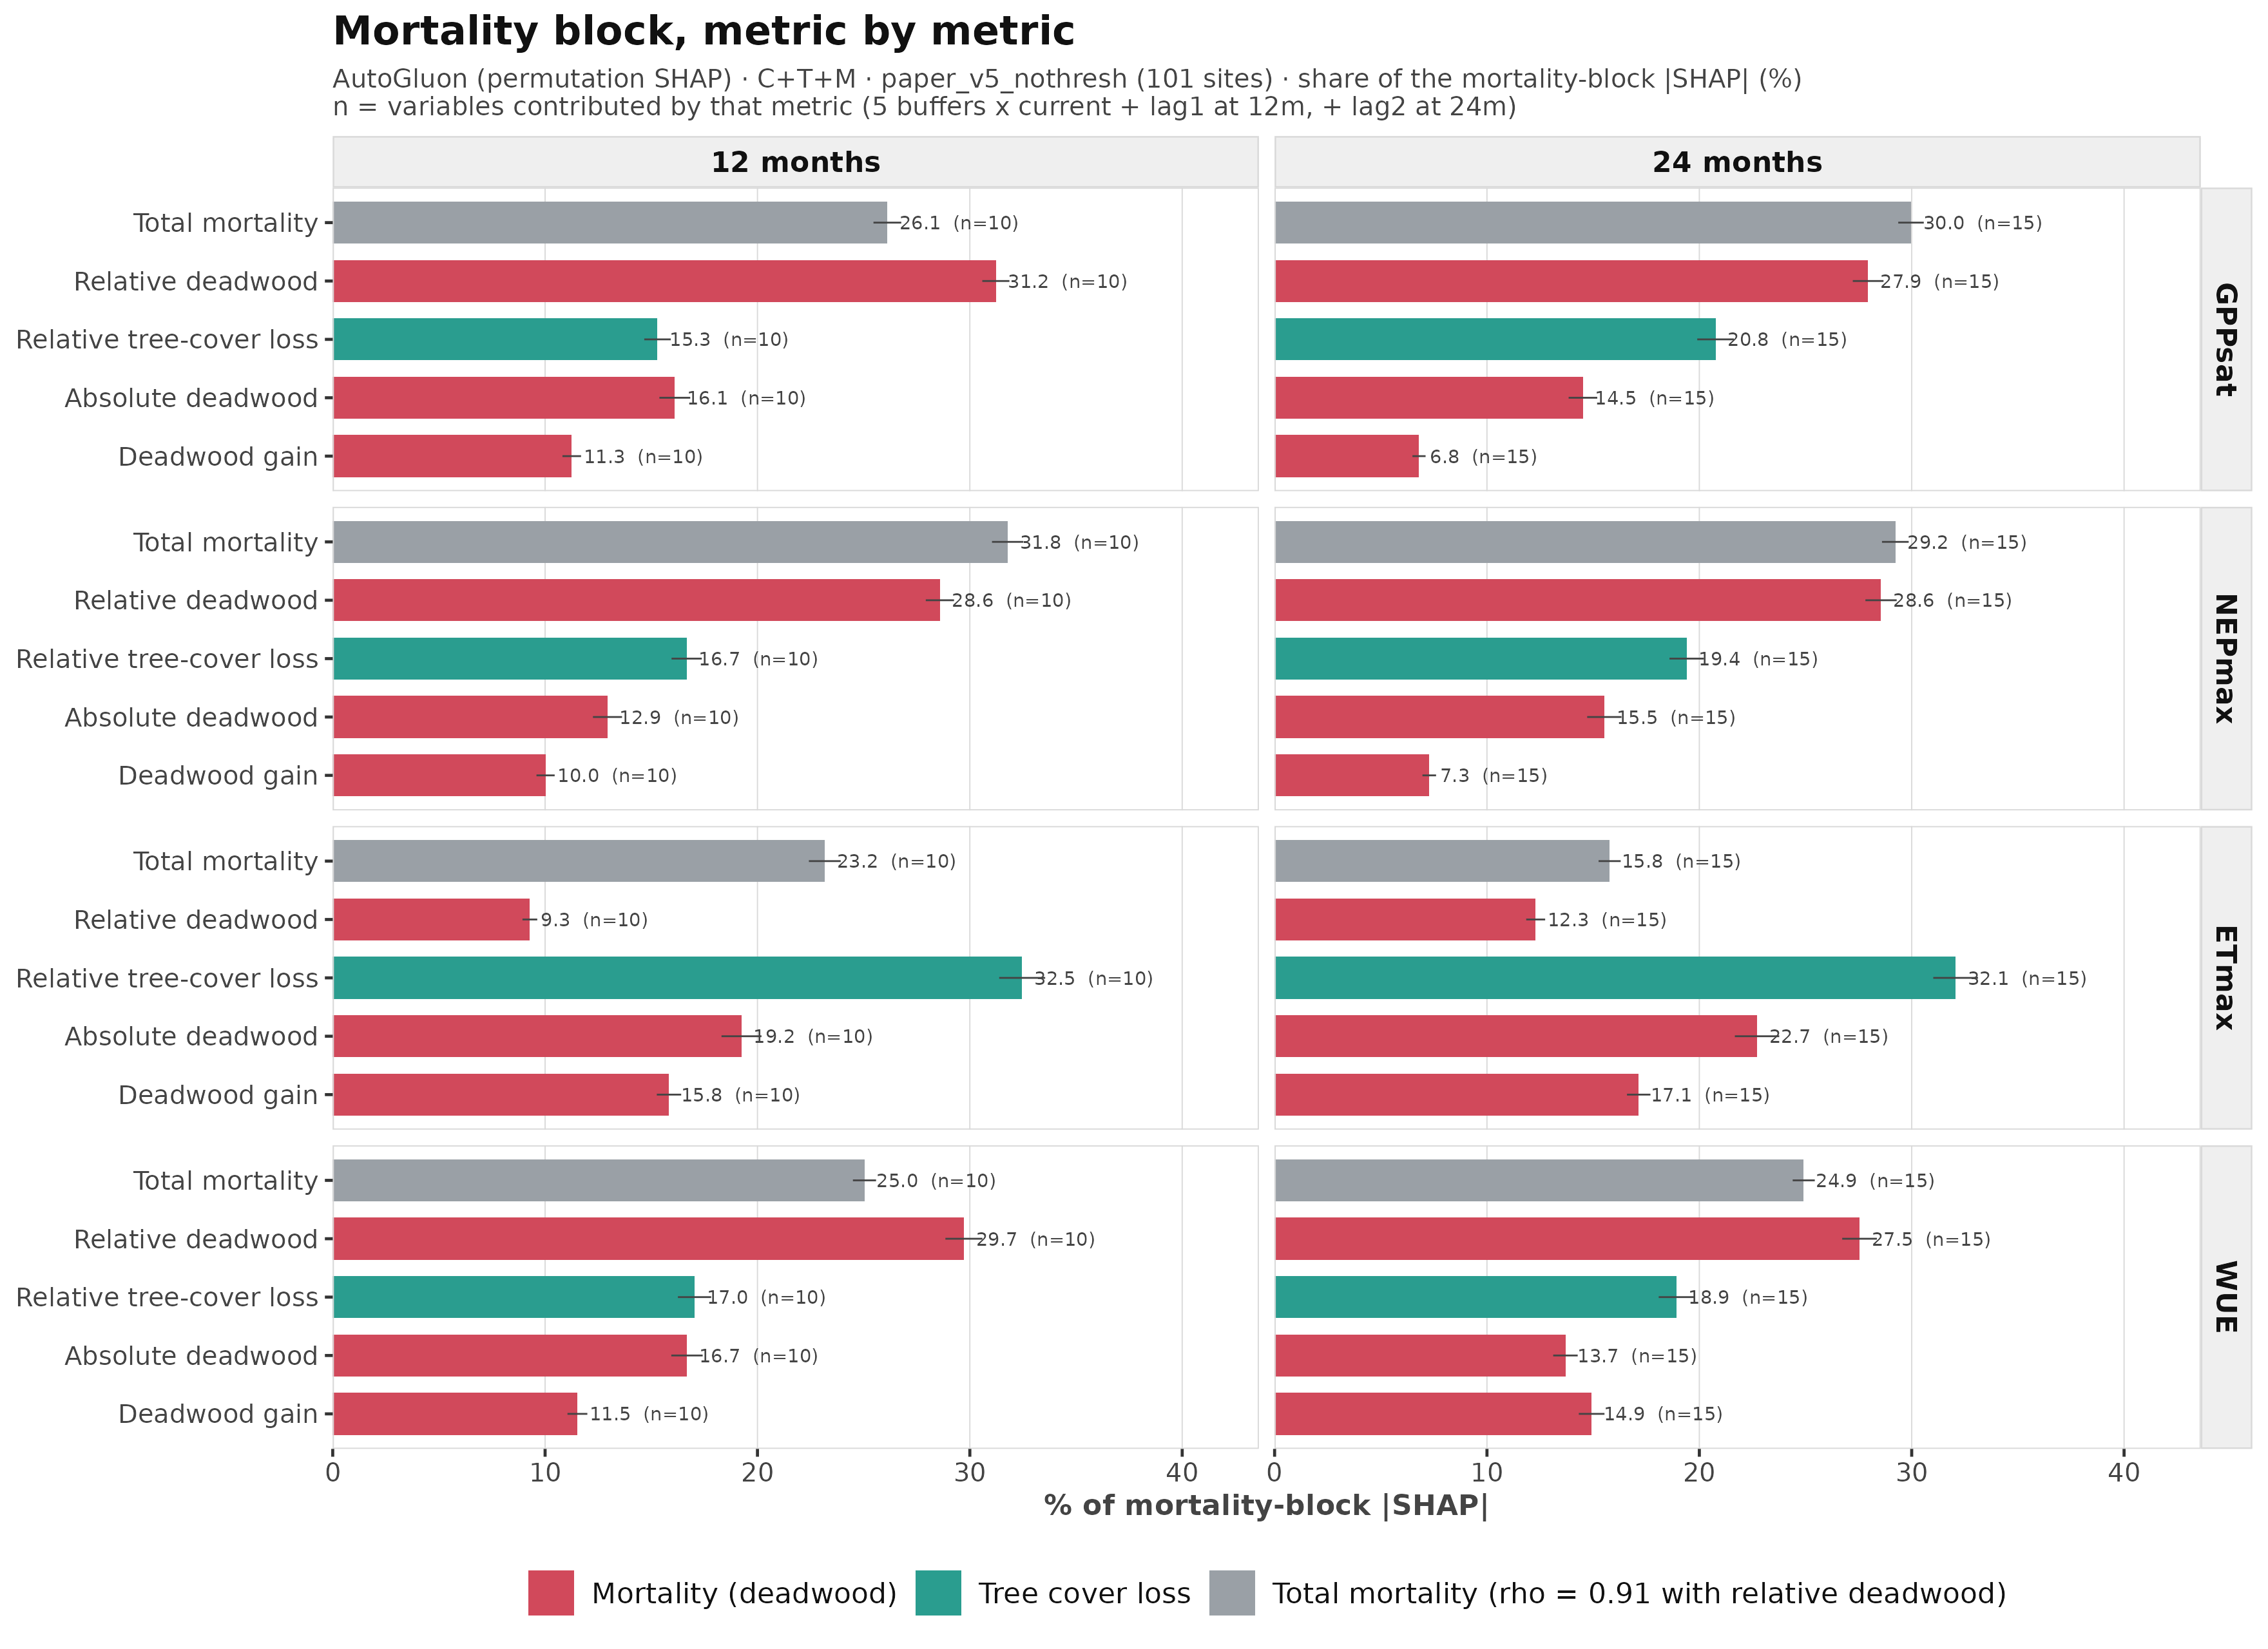
\includegraphics[width=0.8\linewidth]{figures/fig6_mortality_block_AG.png}\\[2pt]
{\small \textbf{Fig.\ 6} --- mortality block metric by metric, AutoGluon (bars $\pm$ SE over sites).}
\end{center}

\section*{Discussions}

 \begin{itemize}
        \item Canopy mortality informs carbon uptake, not water partitioning
        \item The effect is concentrated in the years and sites where mortality happened
        \item The effect is functional, not ecosystem-specific
        \item Site-level heterogeneity and its interpretation
        \item Limitations
        \item Implications
    \end{itemize}
\section*{Conclusions}
\section*{Methods}
\begin{itemize}
  \item \textbf{Dataset:} deadtrees v5 mortality maps, FLUXNET EFPs (GPP$_{sat}$, NEP$_{max}$ following
        Migliavacca et al.\ 2021, ET$_{max}$, WUE), Lusk et al.\ 2025 trait maps (1\,km). Tree cover $\geq$30\,\%
        (500\,m, site mean), EFPs in runs of $\geq$2 consecutive years, CN-Sb1/2 removed by QC:
        \textbf{101 sites, 361 site-years}.
  \item \textbf{Models:} \textbf{climate + traits (C+T)} vs \textbf{climate + traits + mortality (C+T+M)}.
        The pair differs only by the mortality block, so it isolates its contribution.
  \item \textbf{Learner: AutoGluon-Tabular 1.6} (default model zoo: LightGBM, CatBoost, XGBoost, random forest, extra
        trees, two neural networks; weighted ensemble; 5-fold bagging on site-disjoint folds; no stacking). AutoGluon
        is refitted inside every cross-validation fold, so model selection never sees the held-out site. The ensemble
        is dominated by the two neural networks (mean weights 0.43 and 0.32).
  \item \textbf{Check learners (Appendix):} XGBoost and LightGBM, each tuned with Optuna (TPE, 50 trials per
        response and window, grouped 5-fold CV on disjoint site groups).
  \item \textbf{Windows:} climate strictly before the growing season --- 12 months (lag 1) or 24 months (lag 1 + lag 2)
        ending the month before season start; mortality of the current year plus lag 1 (12\,m) or lag 1 + lag 2 (24\,m).
  \item \textbf{Cross-validation:} repeated leave-one-site-out (3 $\times$ 80\,\% of the remaining sites per
        held-out site; predictions averaged over the three repetitions).
  \item \textbf{Mortality predictors:} absolute deadwood, relative deadwood, deadwood gain, relative tree-cover loss
        and total mortality, each at five buffers (100, 200, 300, 400, 500\,m) and the lags above.
  \item \textbf{Site classes} in the figures: site maximum of total mortality across years, mean of the five buffers;
        breaks mean $\pm$ 0.5\,SD (Low $<$ 10.6\,\%, High $>$ 24.0\,\%; 41 Low, 38 Mid, 22 High).
  \item \textbf{Mortality metrics} (from the deadtrees v5 deadwood / tree-cover maps, per buffer):
        \begin{itemize}
          \item \textbf{Absolute deadwood} = standing deadwood / buffer area $\times$ 100 (\%).
          \item \textbf{Relative deadwood} = standing deadwood / tree cover $\times$ 100 (\%), where tree cover $\geq$ 10\,\%, capped at 100\,\%.
          \item \textbf{Total mortality} = (deadwood + tree-cover loss) / (tree cover + tree-cover loss) $\times$ 100 (\%):
                standing dead and removed canopy relative to the canopy present.
        \end{itemize}
  \item \textbf{SHAP:} permutation SHAP for AutoGluon (model-agnostic, approximate); exact TreeSHAP for XGBoost and
        LightGBM. Compare shares and signs between learners, not magnitudes.
  \item \textbf{Statistics:}
        \begin{itemize}
          \item \emph{Site level} (Table~\ref{tab:t1}): per-site MAE (RMSE) over the site's years; one-sided paired
                sign-flip permutation test on the per-site log error ratios (100\,000 flips); effect size =
                geometric-mean change.
          \item \emph{Paired bootstrap} (Table~\ref{tab:t2}): sites resampled with replacement (10\,000 draws, 95\,\%
                percentile interval); at site level the ratio of the mean site errors, at site-year level the ratio of
                the pooled errors over all site-years. Paired permutation with the C+T / C+T+M labels swapped per
                site (all years of a site together).
          \item Fig.~2: one-sided paired Wilcoxon on per-site RMSE (median change). Fig.~4: Mann--Whitney U.
                Fig.~5: Spearman. Benjamini--Hochberg FDR within each table / figure.
        \end{itemize}
  \item Interactive report with all learners and datasets:\\
        \url{https://negin-katal.github.io/fluxVSmortality/v10/index.html}
\end{itemize}

\clearpage
\section*{Appendix}

\subsection*{A1. Learner comparison}
\begin{itemize}
  \item Same data, predictors, windows and cross-validation for all three learners.
  \item AutoGluon best in 7 of 16 tasks; mean $R^2$ (C+T+M) 0.402 / 0.408 (12 / 24\,m) vs XGBoost 0.385 / 0.406
        and LightGBM 0.388 / 0.400.
  \item The effect of mortality is very similar: NEP$_{max}$ improves for every learner; overall RMSE change for
        GPP$_{sat}$ $-2.8$ to $-4.0$\,\% for all learners; AutoGluon gives a somewhat larger WUE effect
        ($-4$\,\% vs $-1$ to $-4$\,\%).
\end{itemize}

\begin{table}[htbp]
\centering
\caption{Skill of the C+T+M model under repeated leave-one-site-out CV ($R^2$), all learners. Bottom rows: mean over the four EFPs.}
\label{tab:a_r2}
\footnotesize
\begin{tabular}{lcccccc}
\toprule
 & \multicolumn{3}{c}{12 months} & \multicolumn{3}{c}{24 months} \\
\cmidrule(lr){2-4}\cmidrule(lr){5-7}
EFP & AutoGluon & XGBoost & LightGBM & AutoGluon & XGBoost & LightGBM \\
\midrule
GPP$_\mathrm{sat}$ & \textbf{0.367} & 0.334 & 0.346 & 0.370 & \textbf{0.387} & 0.347 \\
NEP$_\mathrm{max}$ & \textbf{0.503} & 0.473 & 0.492 & 0.502 & 0.514 & \textbf{0.540} \\
ET$_\mathrm{max}$  & 0.425 & 0.439 & \textbf{0.443} & 0.433 & 0.447 & \textbf{0.453} \\
WUE                & \textbf{0.312} & 0.292 & 0.270 & \textbf{0.326} & 0.277 & 0.261 \\
\midrule
Mean, C+T+M & \textbf{0.402} & 0.385 & 0.388 & \textbf{0.408} & 0.406 & 0.400 \\
Mean, C+T   & \textbf{0.349} & 0.337 & 0.347 & 0.351 & \textbf{0.365} & 0.356 \\
\bottomrule
\end{tabular}
\end{table}

\begin{center}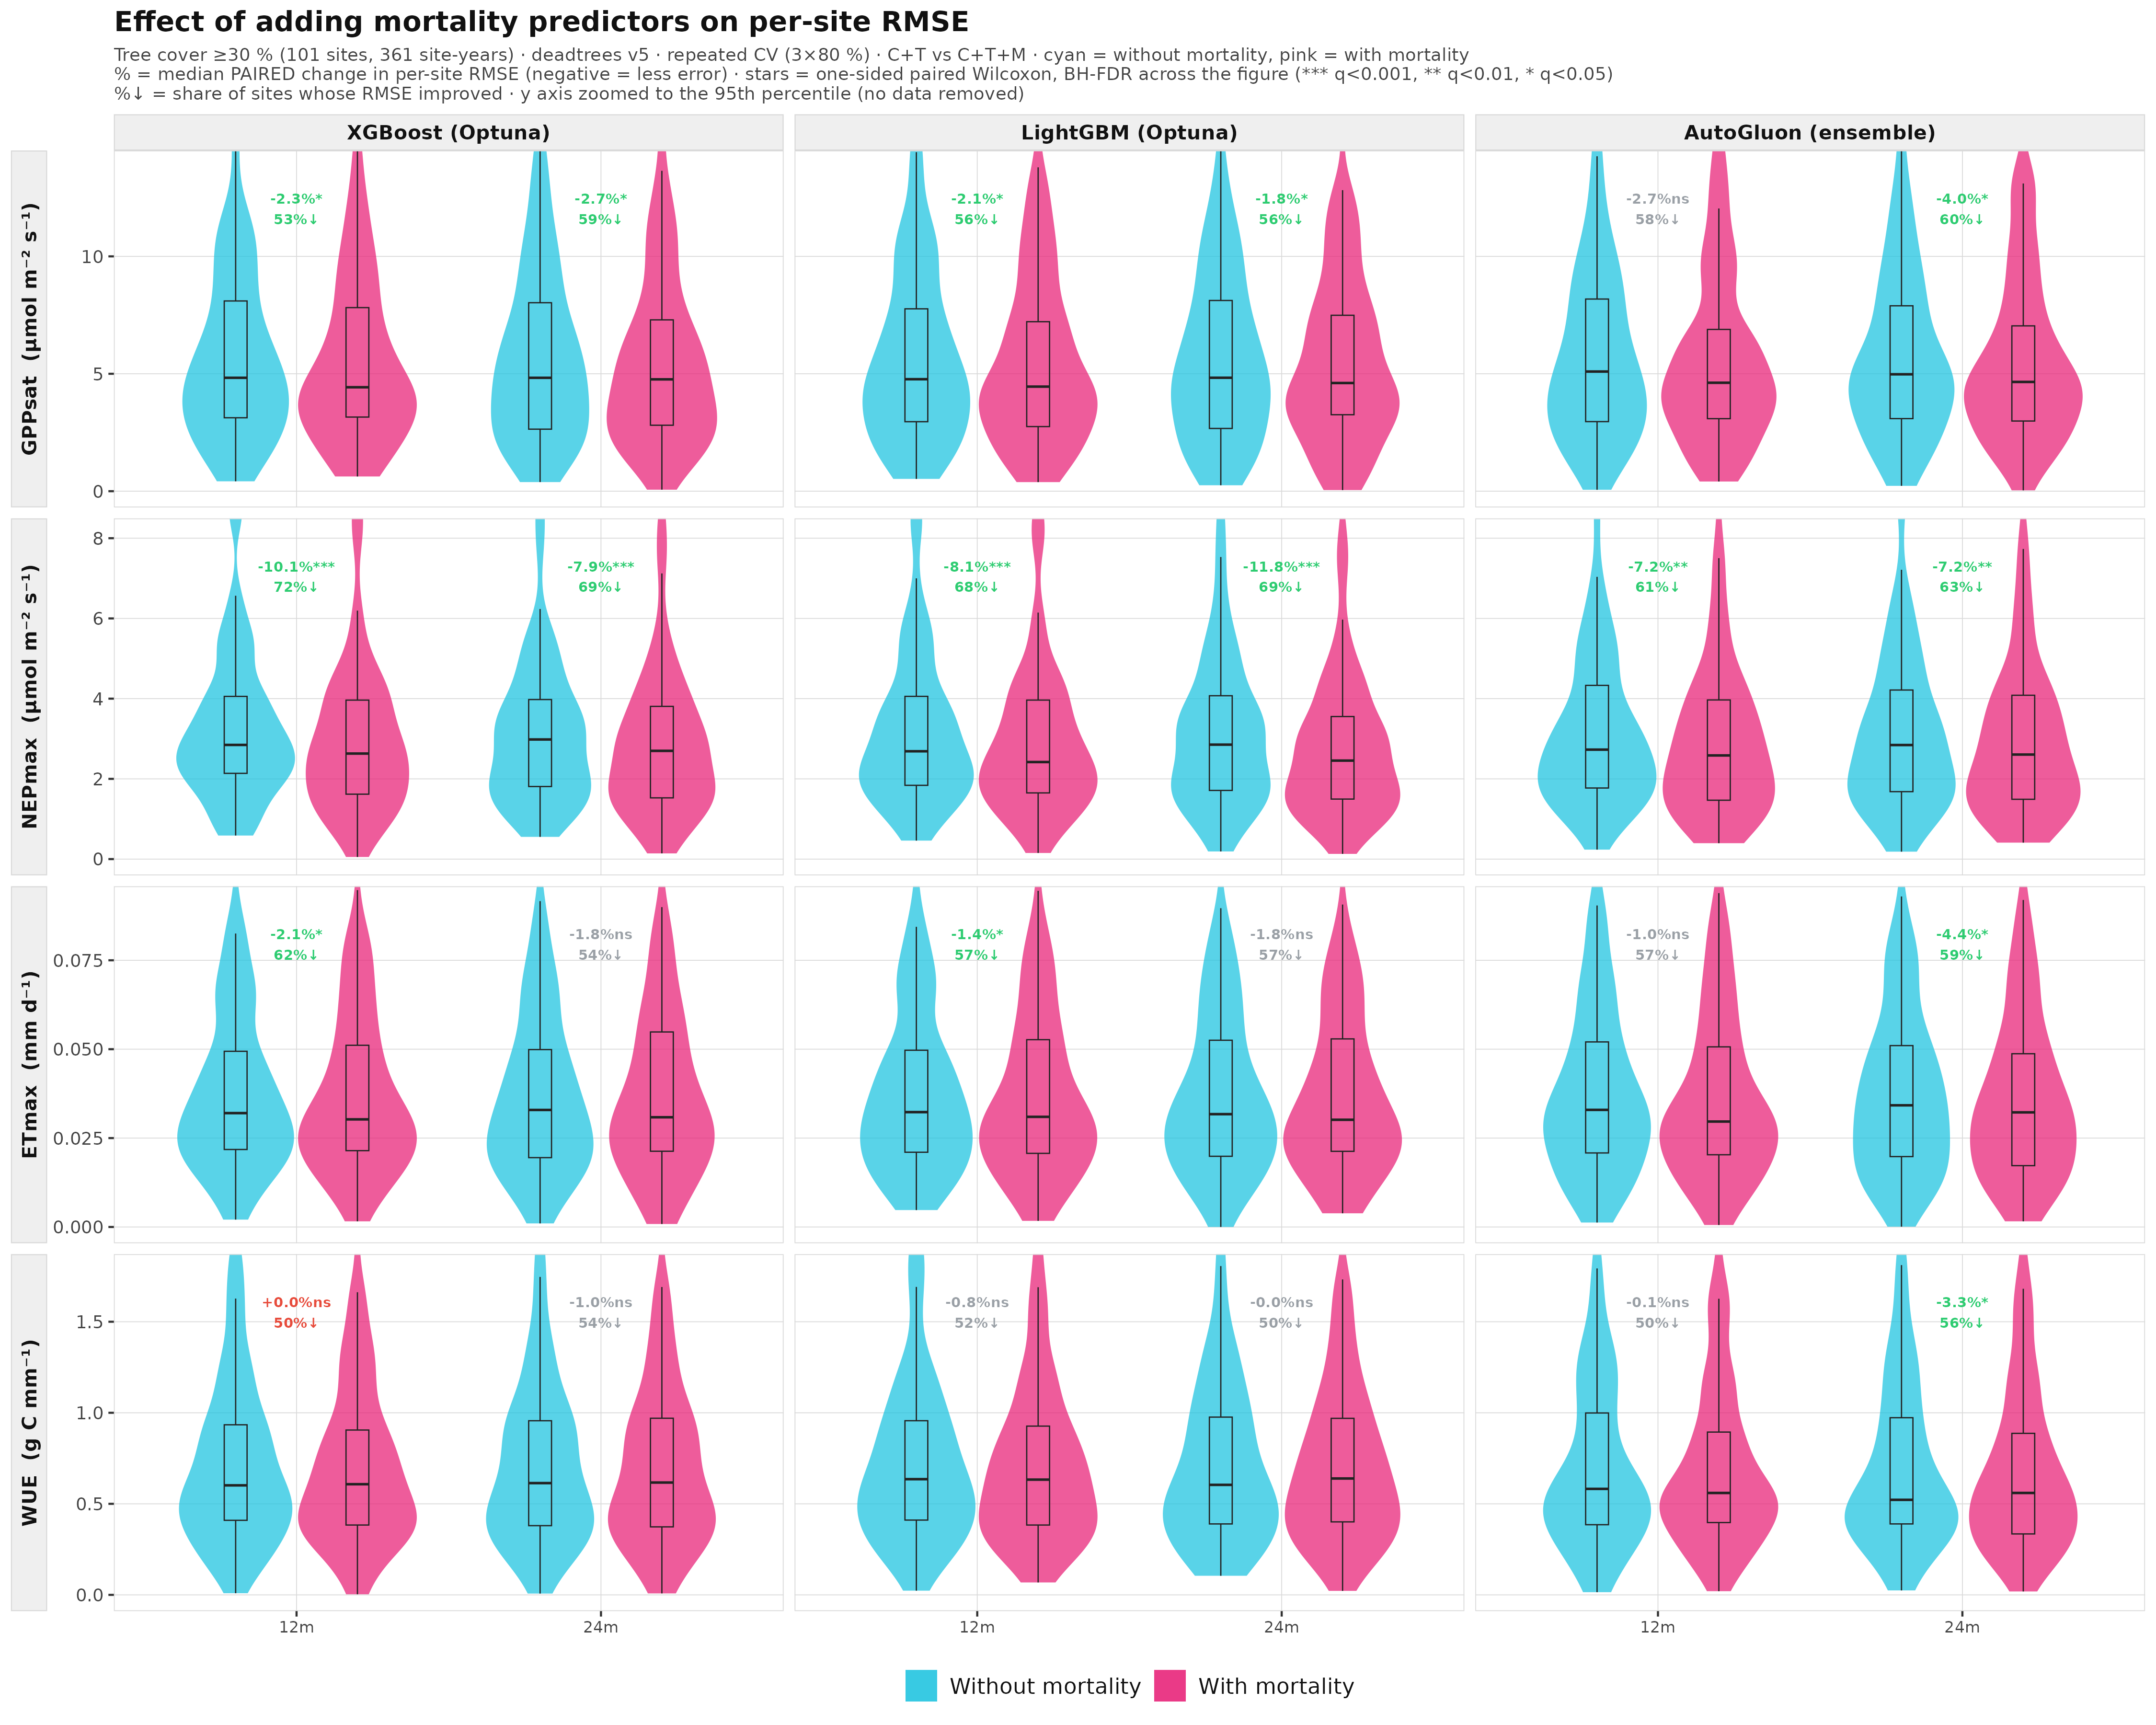
\includegraphics[width=\linewidth]{figures/A_fig2_all_learners.png}\\[2pt]
{\small \textbf{Fig.\ A1} --- Fig.~2a for all three learners.}\end{center}
\begin{center}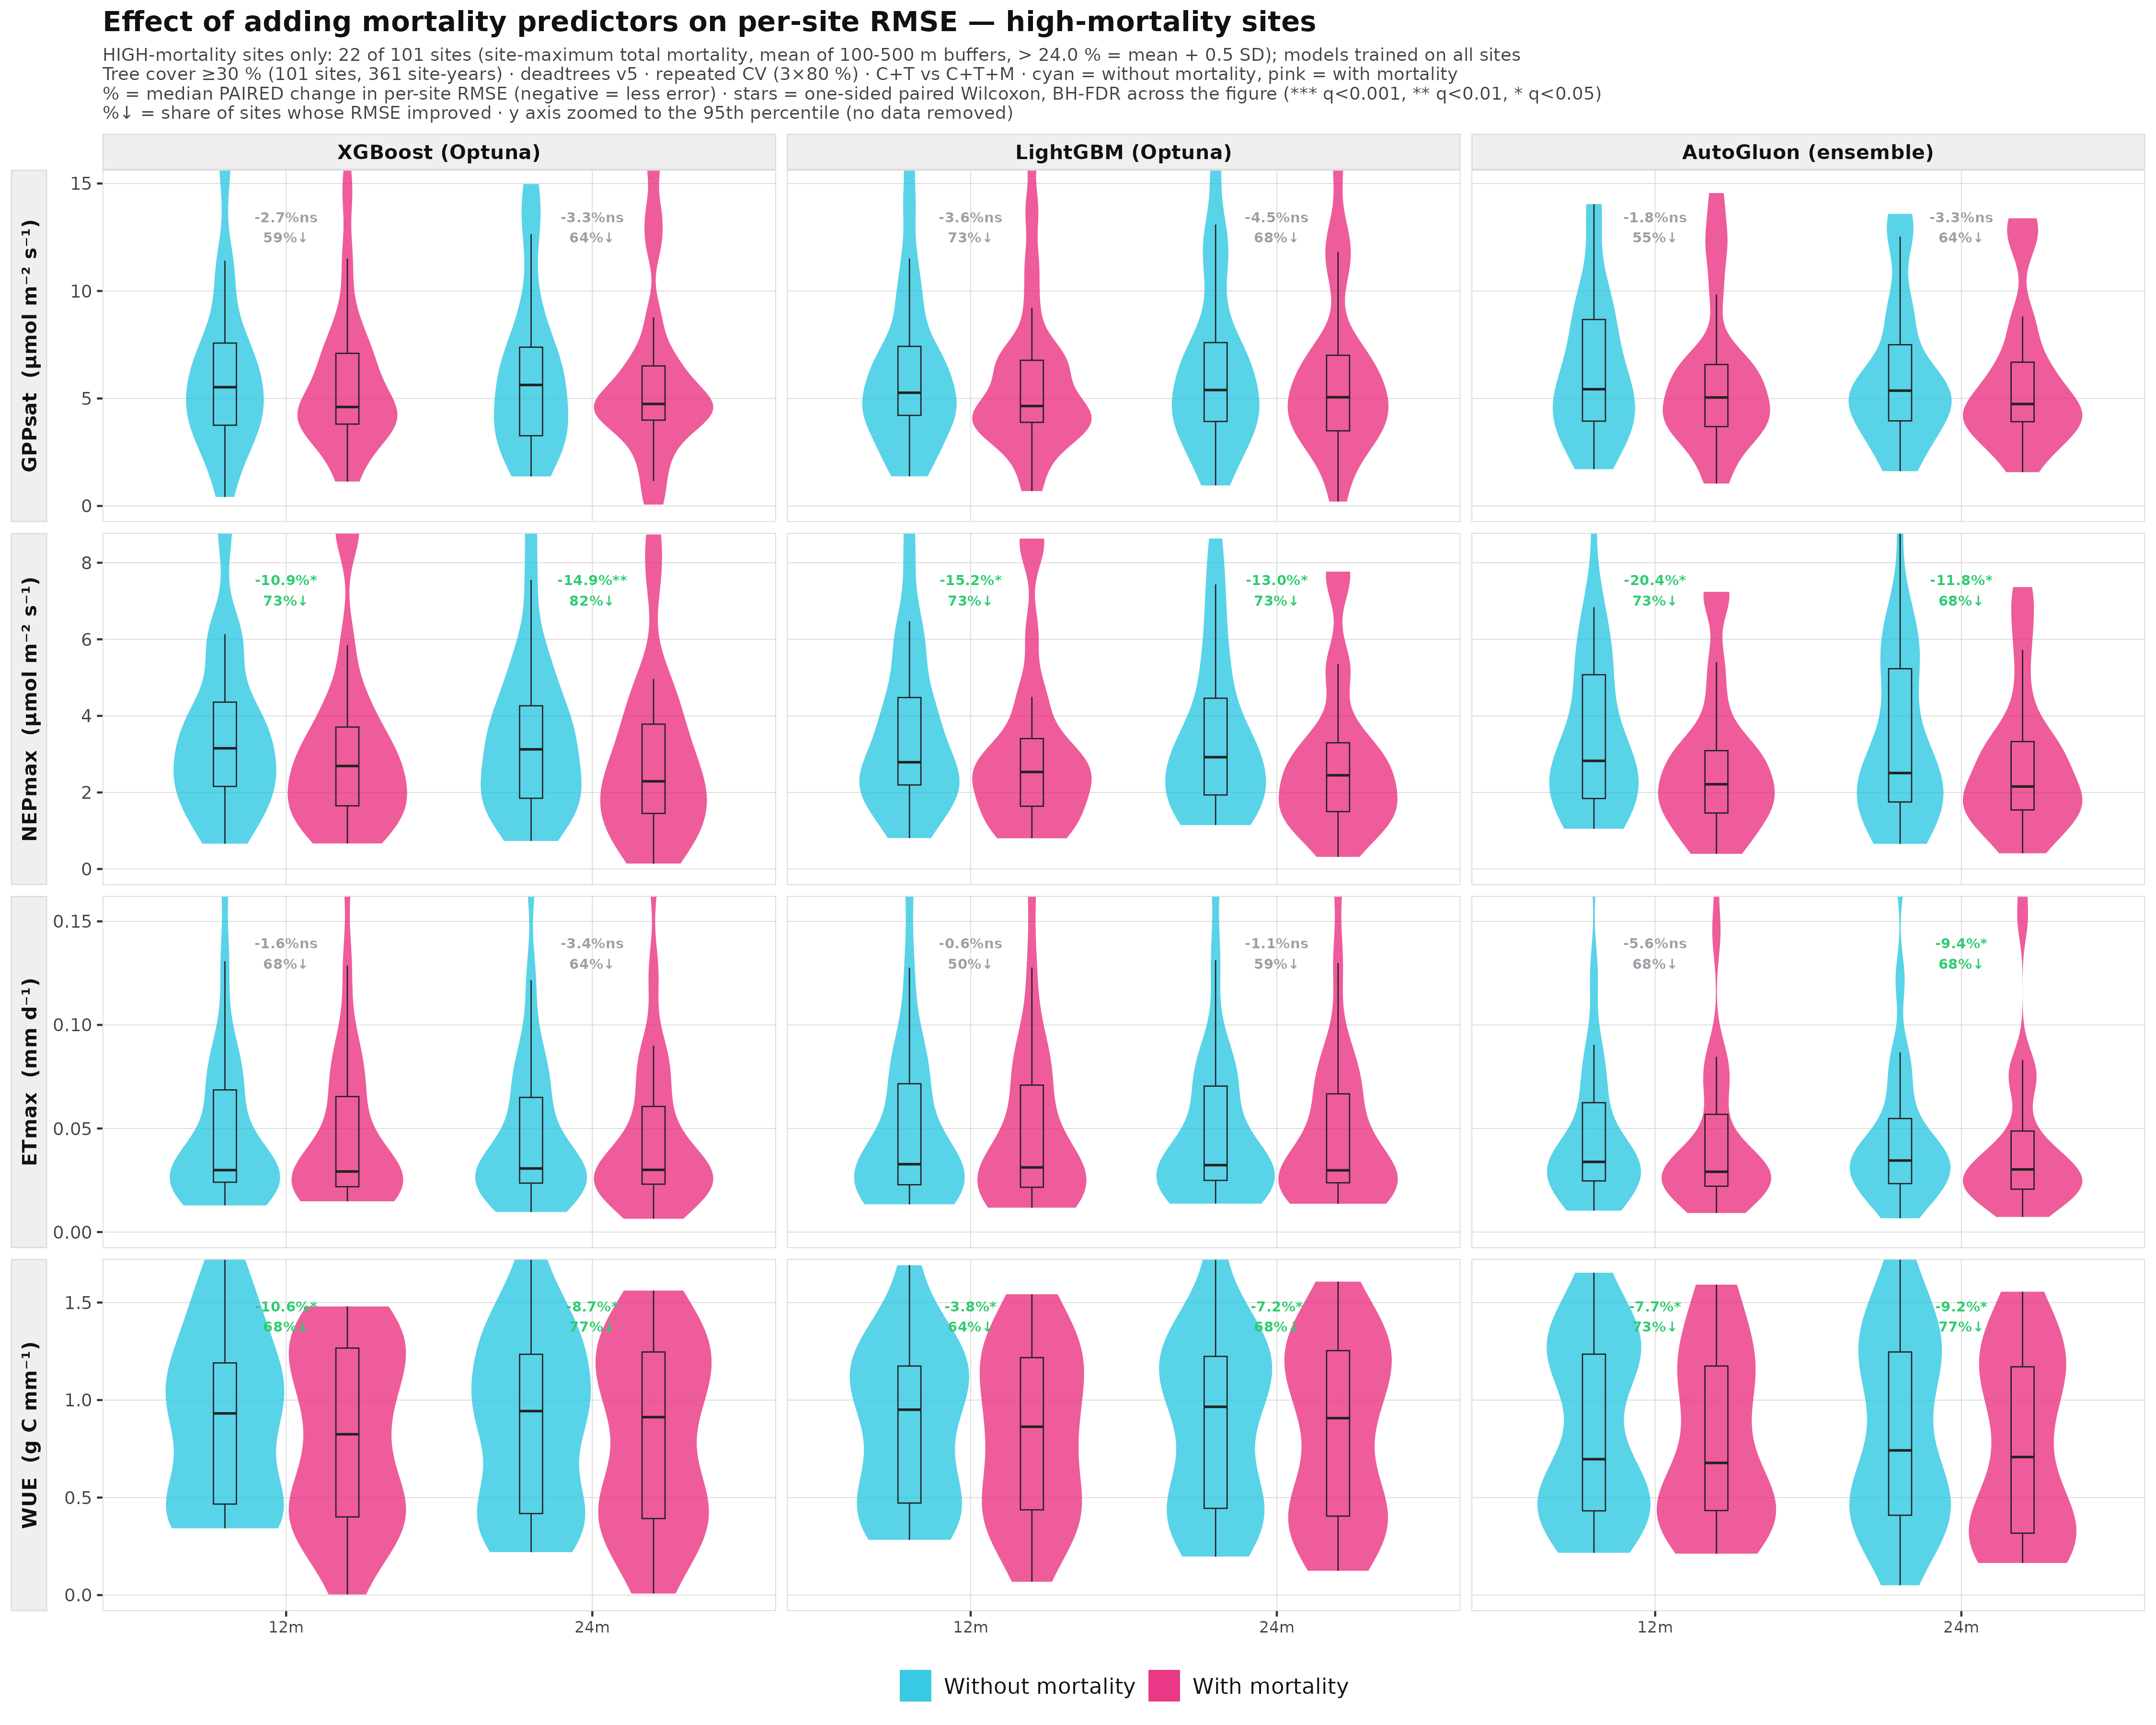
\includegraphics[width=\linewidth]{figures/A_fig2b_high_all_learners.png}\\[2pt]
{\small \textbf{Fig.\ A2} --- Fig.~2b (high total-mortality sites) for all three learners.}\end{center}
\begin{center}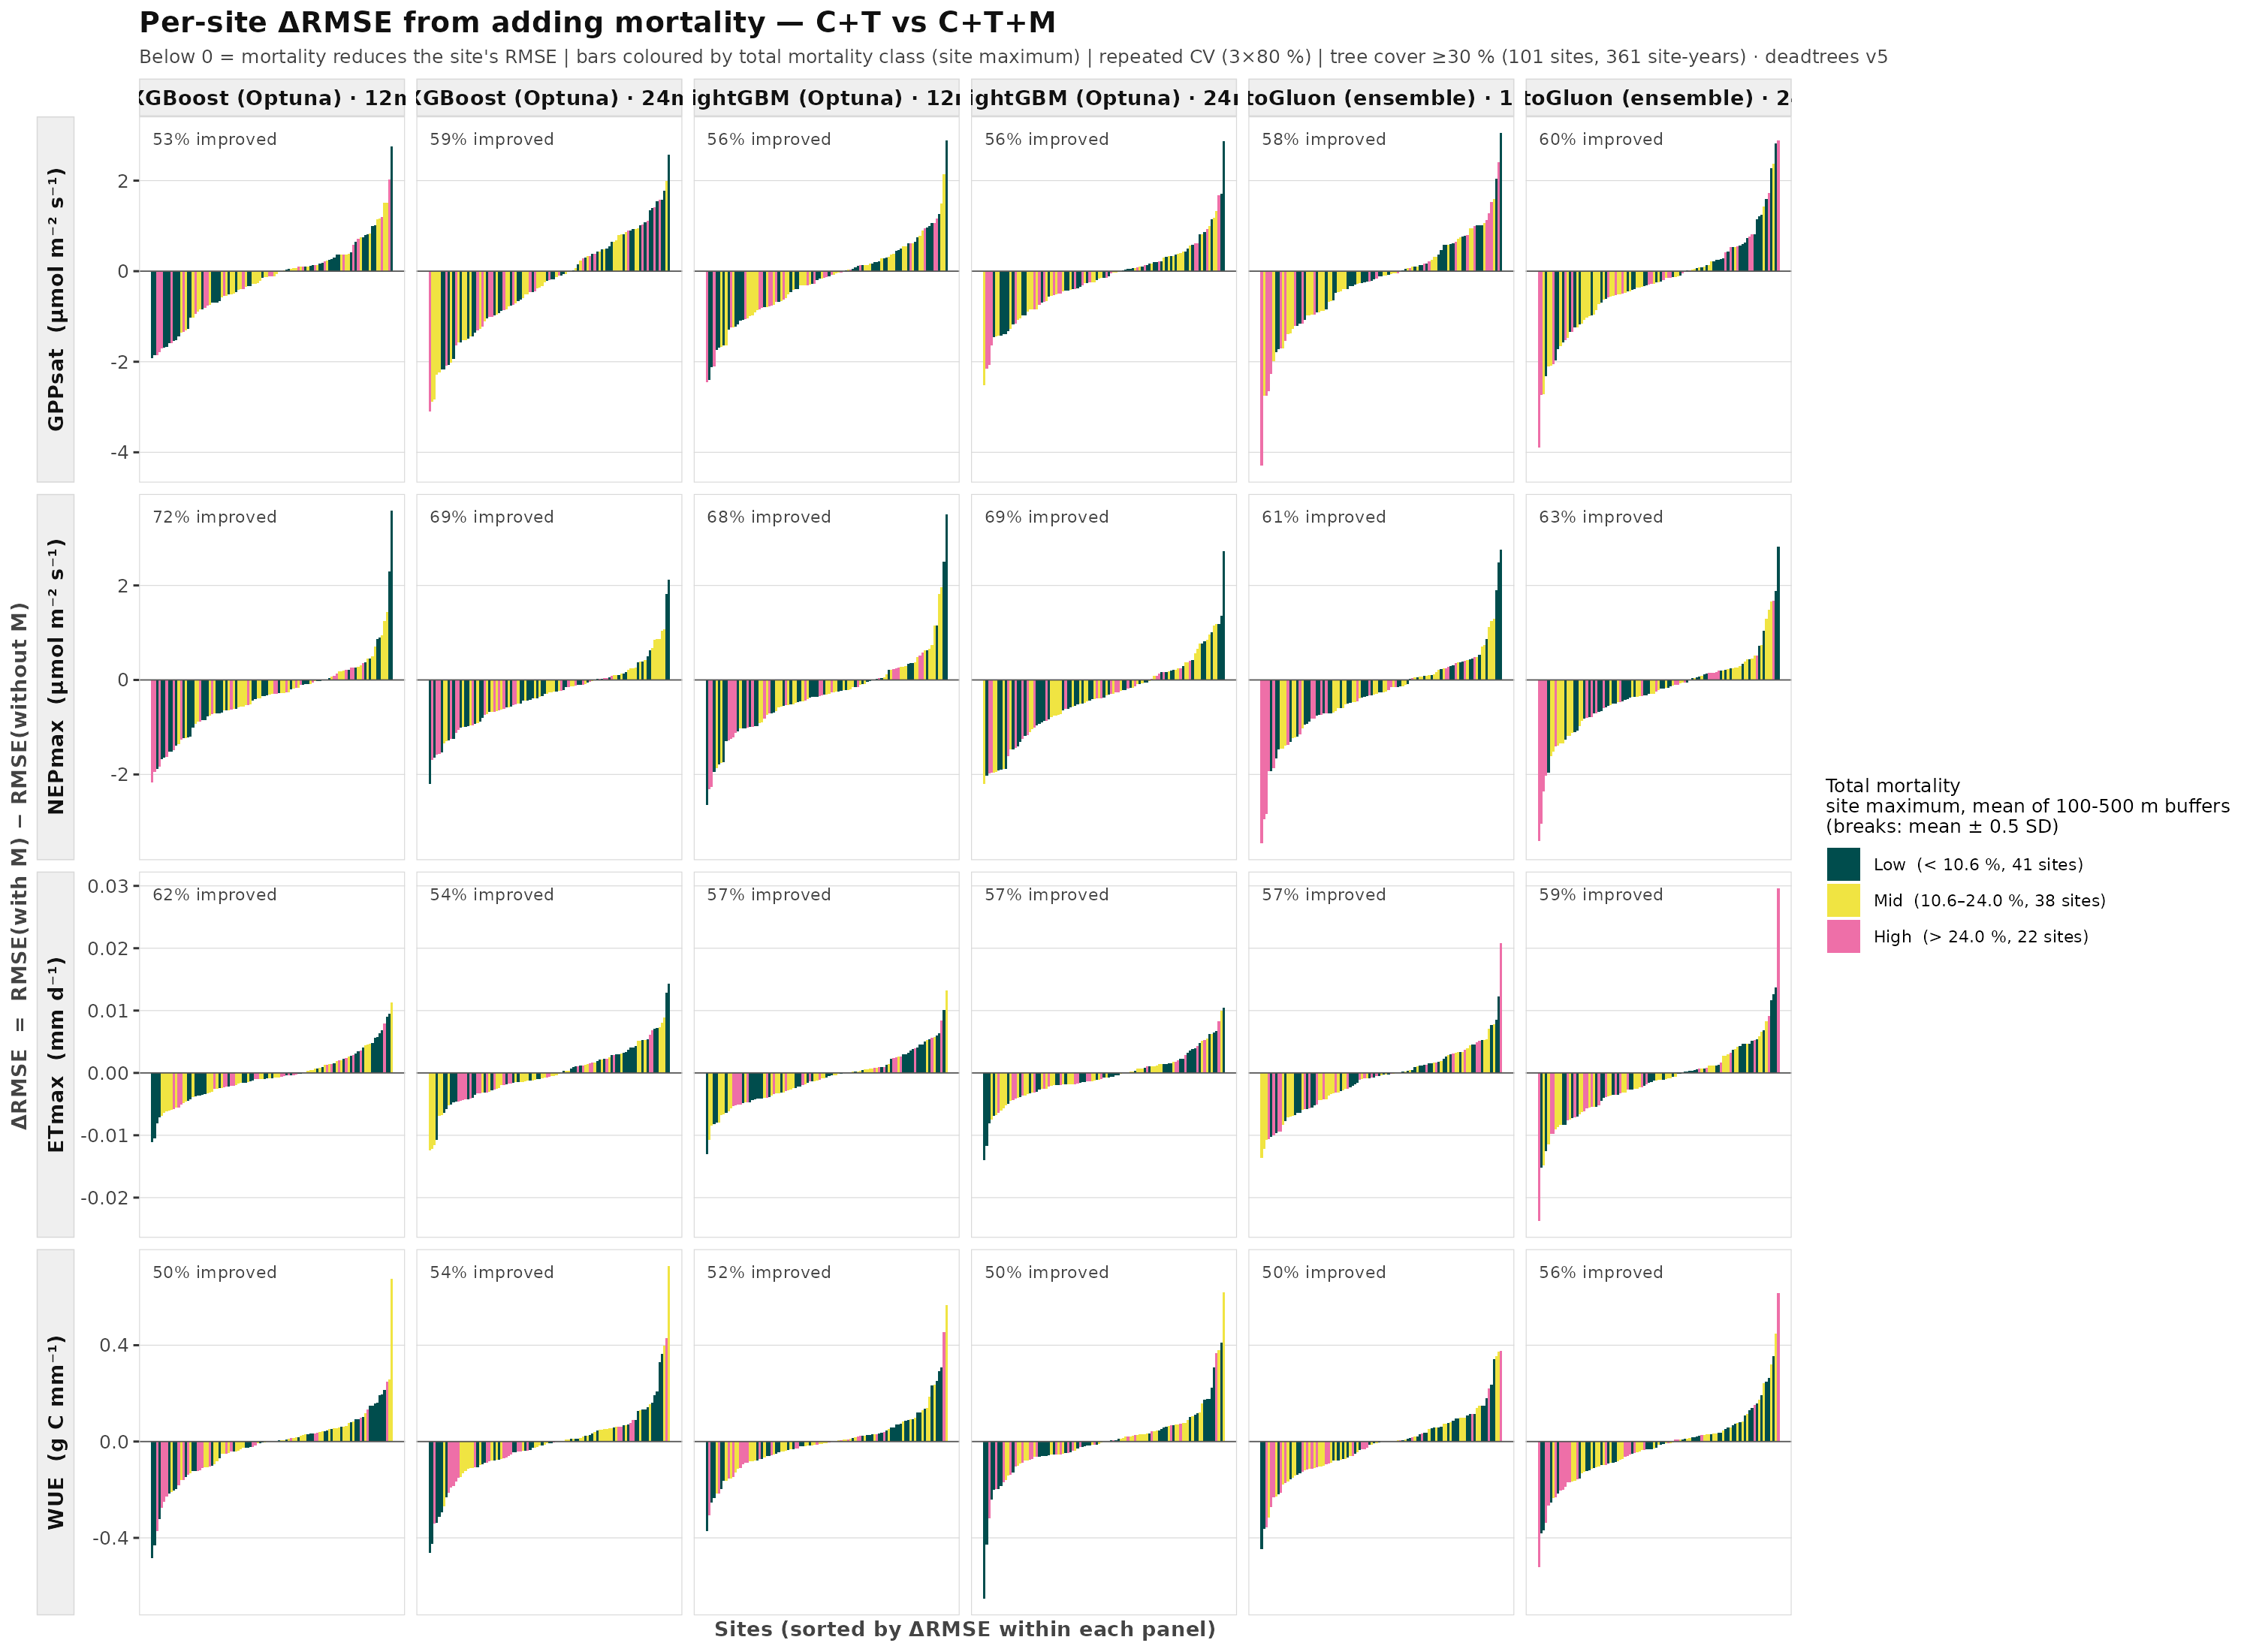
\includegraphics[width=\linewidth]{figures/A_fig2c_site_dRMSE_all_learners.png}\\[2pt]
{\small \textbf{Fig.\ A3} --- Fig.~2c (per-site $\Delta$RMSE) for all three learners.}\end{center}

\subsection*{A2. Tables~\ref{tab:t1}--\ref{tab:t2} with RMSE and for XGBoost / LightGBM}
\begin{table}[htbp]
\centering
\caption{Effect of adding mortality predictors on per-site prediction error (summary of Fig.~2). For every site, RMSE of the model with climate, traits and mortality (C+T+M) is compared with the model without mortality (C+T), both evaluated by repeated leave-one-site-out cross-validation (3 $\times$ 80\%). $\Delta$RMSE = geometric mean over sites of the paired error ratio, (exp(mean$_\mathrm{sites}$ ln(RMSE$_\mathrm{C+T+M}$ / RMSE$_\mathrm{C+T}$)) $-$ 1) $\times$ 100; negative values mean that mortality reduces the error. Improved = share of sites whose RMSE decreased. Sites are grouped by their maximum total mortality across years (averaged over the five buffers, 100--500\,m); High $>$ mean $+$ 0.5\,SD (24.0\%), Low $<$ mean $-$ 0.5\,SD (10.6\%), Mid in between. Stars: one-sided paired permutation test on the per-site log error ratios (100\,000 random sign flips; C+T+M $<$ C+T), Benjamini--Hochberg corrected across all 72 tests of the three learners ($^{*}$\,$q<0.05$, $^{**}$\,$q<0.01$, $^{***}$\,$q<0.001$). Tree cover $\geq$ 30\%, 101 sites, 361 site-years, deadtrees v5.}
\label{tab:a1}
\scriptsize
\setlength{\tabcolsep}{4pt}
\renewcommand{\arraystretch}{0.92}
\begin{tabular}{lllccc}
\toprule
Model & EFP & & All sites & Mid + High & High \\
 & & & ($n$ = 101) & ($n$ = 60) & ($n$ = 22) \\
\midrule
\multirow{8}{*}{\shortstack[l]{AutoGluon\\12\,months}} & \multirow{2}{*}{GPP$_\mathrm{sat}$} & $\Delta$RMSE (\%) & $-2.8$ & $-7.2$$^{*}$ & $-9.8$ \\
 & & Improved (\%) & 58 & 62 & 55 \\
\cmidrule(l){2-6}
 & \multirow{2}{*}{NEP$_\mathrm{max}$} & $\Delta$RMSE (\%) & $-11.3$$^{*}$ & $-14.5$$^{**}$ & $-28.7$$^{**}$ \\
 & & Improved (\%) & 61 & 62 & 73 \\
\cmidrule(l){2-6}
 & \multirow{2}{*}{ET$_\mathrm{max}$} & $\Delta$RMSE (\%) & $-4.3$ & $-4.9$ & $-5.0$ \\
 & & Improved (\%) & 57 & 63 & 68 \\
\cmidrule(l){2-6}
 & \multirow{2}{*}{WUE} & $\Delta$RMSE (\%) & $+2.3$ & $-2.9$ & $-7.8$ \\
 & & Improved (\%) & 50 & 60 & 73 \\
\midrule
\multirow{8}{*}{\shortstack[l]{AutoGluon\\24\,months}} & \multirow{2}{*}{GPP$_\mathrm{sat}$} & $\Delta$RMSE (\%) & $-5.0$ & $-7.3$$^{*}$ & $-4.6$ \\
 & & Improved (\%) & 60 & 70 & 64 \\
\cmidrule(l){2-6}
 & \multirow{2}{*}{NEP$_\mathrm{max}$} & $\Delta$RMSE (\%) & $-6.9$ & $-9.3$ & $-18.2$ \\
 & & Improved (\%) & 63 & 62 & 68 \\
\cmidrule(l){2-6}
 & \multirow{2}{*}{ET$_\mathrm{max}$} & $\Delta$RMSE (\%) & $-2.6$ & $-6.1$ & $-9.4$ \\
 & & Improved (\%) & 59 & 65 & 68 \\
\cmidrule(l){2-6}
 & \multirow{2}{*}{WUE} & $\Delta$RMSE (\%) & $-1.6$ & $-4.7$ & $-11.1$ \\
 & & Improved (\%) & 56 & 63 & 77 \\
\bottomrule
\end{tabular}
\end{table}

\begin{table}[htbp]
\centering
\caption{Paired bootstrap of the change in RMSE when mortality is added (C+T $\rightarrow$ C+T+M), AutoGluon. Cells: \% change of the error, 100\,(RMSE$_\mathrm{C+T+M}$ / RMSE$_\mathrm{C+T}$ $-$ 1), with the 95\,\% bootstrap interval in brackets. \emph{Site level}: one RMSE per site and model over its years, ratio of the mean site errors. \emph{Site-year level}: every site-year is an observation (pooled RMSE; no averaging over years). Years of one site are not independent, so at both levels whole sites are resampled (10\,000 bootstrap draws) and the C+T / C+T+M labels are swapped per site for the paired permutation test (10\,000 draws, one-sided; stars, Benjamini--Hochberg corrected across all three learners: $^{*}$\,$q<0.05$, $^{**}$\,$q<0.01$, $^{***}$\,$q<0.001$). High sites: site maximum of total mortality $>$ 24.0\,\%; the last two columns keep only the site-years whose own total mortality exceeds 10.6\,\% (Mid + High) or 24.0\,\% (High). Column heads: sites / site-years. 101 sites, 361 site-years, deadtrees v5.}
\label{tab:a2}
\scriptsize
\setlength{\tabcolsep}{3pt}
\resizebox{\linewidth}{!}{%
\begin{tabular}{llccccc}
\toprule
 & & Site level & \multicolumn{4}{c}{Site-year level} \\
\cmidrule(lr){3-3}\cmidrule(lr){4-7}
 & & All sites & All sites & High sites & Mid + High years & High years \\
 & & (101 sites) & (101 / 361) & (22 / 80) & (60 / 160) & (22 / 40) \\
\midrule
\multirow{4}{*}{\shortstack[l]{AutoGluon\\12\,months}} & GPP$_\mathrm{sat}$ & $-3.6$ {\tiny[$-7.2$, $+0.1$]} & $-2.8$ {\tiny[$-6.1$, $+0.5$]} & $-4.4$ {\tiny[$-15.2$, $+4.5$]} & $-4.4$ {\tiny[$-10.0$, $+0.9$]} & $-10.1$ {\tiny[$-27.6$, $+5.8$]} \\
 & NEP$_\mathrm{max}$ & $-9.3$ {\tiny[$-14.4$, $-3.9$]}$^{**}$ & $-9.7$ {\tiny[$-14.6$, $-4.7$]}$^{**}$ & $-21.0$ {\tiny[$-33.7$, $-7.7$]}$^{*}$ & $-11.8$ {\tiny[$-19.7$, $-4.3$]}$^{*}$ & $-32.6$ {\tiny[$-45.1$, $-16.0$]}$^{*}$ \\
 & ET$_\mathrm{max}$ & $-2.4$ {\tiny[$-5.1$, $+0.3$]} & $-0.2$ {\tiny[$-2.6$, $+2.1$]} & $+0.0$ {\tiny[$-5.9$, $+5.6$]} & $-0.7$ {\tiny[$-4.7$, $+3.5$]} & $-0.7$ {\tiny[$-17.2$, $+17.2$]} \\
 & WUE & $-2.2$ {\tiny[$-6.0$, $+1.8$]} & $-4.1$ {\tiny[$-7.3$, $-1.2$]}$^{*}$ & $-7.5$ {\tiny[$-14.3$, $-1.5$]}$^{*}$ & $-5.7$ {\tiny[$-10.3$, $-1.4$]}$^{*}$ & $-14.3$ {\tiny[$-22.3$, $-2.7$]} \\
\midrule
\multirow{4}{*}{\shortstack[l]{AutoGluon\\24\,months}} & GPP$_\mathrm{sat}$ & $-4.3$ {\tiny[$-7.9$, $-0.6$]}$^{*}$ & $-4.0$ {\tiny[$-7.3$, $-0.2$]}$^{*}$ & $-4.2$ {\tiny[$-14.0$, $+4.7$]} & $-6.0$ {\tiny[$-11.2$, $-1.2$]}$^{*}$ & $-9.8$ {\tiny[$-25.4$, $+7.0$]} \\
 & NEP$_\mathrm{max}$ & $-8.3$ {\tiny[$-13.3$, $-2.9$]}$^{**}$ & $-9.4$ {\tiny[$-14.2$, $-4.2$]}$^{*}$ & $-19.5$ {\tiny[$-32.3$, $-5.7$]}$^{*}$ & $-11.8$ {\tiny[$-19.5$, $-3.8$]}$^{*}$ & $-31.0$ {\tiny[$-44.0$, $-13.1$]}$^{*}$ \\
 & ET$_\mathrm{max}$ & $-3.1$ {\tiny[$-6.3$, $+0.2$]} & $-0.4$ {\tiny[$-3.1$, $+2.6$]} & $+0.6$ {\tiny[$-7.8$, $+7.9$]} & $-1.6$ {\tiny[$-6.4$, $+2.9$]} & $+0.4$ {\tiny[$-19.3$, $+22.0$]} \\
 & WUE & $-3.0$ {\tiny[$-7.2$, $+1.6$]} & $-4.3$ {\tiny[$-7.4$, $-1.2$]}$^{*}$ & $-9.2$ {\tiny[$-16.3$, $-2.4$]}$^{*}$ & $-6.7$ {\tiny[$-11.4$, $-1.5$]}$^{*}$ & $-16.9$ {\tiny[$-24.6$, $-6.5$]}$^{*}$ \\
\bottomrule
\end{tabular}}
\end{table}

\begin{table}[p]
\centering
\caption{Effect of adding mortality predictors on per-site prediction error (summary of Fig.~2). For every site, MAE of the model with climate, traits and mortality (C+T+M) is compared with the model without mortality (C+T), both evaluated by repeated leave-one-site-out cross-validation (3 $\times$ 80\%). $\Delta$MAE = geometric mean over sites of the paired error ratio, (exp(mean$_\mathrm{sites}$ ln(MAE$_\mathrm{C+T+M}$ / MAE$_\mathrm{C+T}$)) $-$ 1) $\times$ 100; negative values mean that mortality reduces the error. Improved = share of sites whose MAE decreased. Sites are grouped by their maximum total mortality across years (averaged over the five buffers, 100--500\,m); High $>$ mean $+$ 0.5\,SD (24.0\%), Low $<$ mean $-$ 0.5\,SD (10.6\%), Mid in between. Stars: one-sided paired permutation test on the per-site log error ratios (100\,000 random sign flips; C+T+M $<$ C+T), Benjamini--Hochberg corrected across all 72 tests of the three learners ($^{*}$\,$q<0.05$, $^{**}$\,$q<0.01$, $^{***}$\,$q<0.001$). Tree cover $\geq$ 30\%, 101 sites, 361 site-years, deadtrees v5.}
\label{tab:a3}
\scriptsize
\setlength{\tabcolsep}{4pt}
\renewcommand{\arraystretch}{0.92}
\begin{tabular}{lllccc}
\toprule
Model & EFP & & All sites & Mid + High & High \\
 & & & ($n$ = 101) & ($n$ = 60) & ($n$ = 22) \\
\midrule
\multirow{8}{*}{\shortstack[l]{XGBoost\\12\,months}} & \multirow{2}{*}{GPP$_\mathrm{sat}$} & $\Delta$MAE (\%) & $-2.5$ & $+1.4$ & $+0.2$ \\
 & & Improved (\%) & 54 & 57 & 59 \\
\cmidrule(l){2-6}
 & \multirow{2}{*}{NEP$_\mathrm{max}$} & $\Delta$MAE (\%) & $-15.1$$^{**}$ & $-13.0$$^{**}$ & $-18.4$$^{*}$ \\
 & & Improved (\%) & 70 & 68 & 73 \\
\cmidrule(l){2-6}
 & \multirow{2}{*}{ET$_\mathrm{max}$} & $\Delta$MAE (\%) & $-1.2$ & $-3.9$ & $-0.5$ \\
 & & Improved (\%) & 59 & 63 & 64 \\
\cmidrule(l){2-6}
 & \multirow{2}{*}{WUE} & $\Delta$MAE (\%) & $-4.9$ & $-6.8$ & $-25.2$$^{*}$ \\
 & & Improved (\%) & 52 & 53 & 68 \\
\midrule
\multirow{8}{*}{\shortstack[l]{XGBoost\\24\,months}} & \multirow{2}{*}{GPP$_\mathrm{sat}$} & $\Delta$MAE (\%) & $-6.9$ & $-12.7$$^{*}$ & $-18.7$ \\
 & & Improved (\%) & 61 & 65 & 68 \\
\cmidrule(l){2-6}
 & \multirow{2}{*}{NEP$_\mathrm{max}$} & $\Delta$MAE (\%) & $-15.5$$^{**}$ & $-16.5$$^{**}$ & $-29.4$$^{**}$ \\
 & & Improved (\%) & 68 & 63 & 73 \\
\cmidrule(l){2-6}
 & \multirow{2}{*}{ET$_\mathrm{max}$} & $\Delta$MAE (\%) & $-2.0$ & $-3.1$ & $-5.0$ \\
 & & Improved (\%) & 54 & 63 & 68 \\
\cmidrule(l){2-6}
 & \multirow{2}{*}{WUE} & $\Delta$MAE (\%) & $-2.9$ & $-3.9$ & $-20.9$ \\
 & & Improved (\%) & 54 & 57 & 68 \\
\midrule
\multirow{8}{*}{\shortstack[l]{LightGBM\\12\,months}} & \multirow{2}{*}{GPP$_\mathrm{sat}$} & $\Delta$MAE (\%) & $-3.7$ & $-2.6$ & $-8.5$ \\
 & & Improved (\%) & 54 & 58 & 68 \\
\cmidrule(l){2-6}
 & \multirow{2}{*}{NEP$_\mathrm{max}$} & $\Delta$MAE (\%) & $-12.1$$^{**}$ & $-10.6$$^{*}$ & $-17.9$$^{*}$ \\
 & & Improved (\%) & 70 & 70 & 77 \\
\cmidrule(l){2-6}
 & \multirow{2}{*}{ET$_\mathrm{max}$} & $\Delta$MAE (\%) & $-4.2$ & $-5.8$ & $-1.3$ \\
 & & Improved (\%) & 56 & 62 & 50 \\
\cmidrule(l){2-6}
 & \multirow{2}{*}{WUE} & $\Delta$MAE (\%) & $+2.4$ & $-2.0$ & $-9.6$ \\
 & & Improved (\%) & 52 & 62 & 55 \\
\midrule
\multirow{8}{*}{\shortstack[l]{LightGBM\\24\,months}} & \multirow{2}{*}{GPP$_\mathrm{sat}$} & $\Delta$MAE (\%) & $-6.5$ & $-7.1$$^{*}$ & $-10.6$ \\
 & & Improved (\%) & 58 & 62 & 64 \\
\cmidrule(l){2-6}
 & \multirow{2}{*}{NEP$_\mathrm{max}$} & $\Delta$MAE (\%) & $-13.3$$^{*}$ & $-16.6$$^{**}$ & $-22.1$$^{*}$ \\
 & & Improved (\%) & 65 & 63 & 68 \\
\cmidrule(l){2-6}
 & \multirow{2}{*}{ET$_\mathrm{max}$} & $\Delta$MAE (\%) & $+3.7$ & $-1.2$ & $-1.1$ \\
 & & Improved (\%) & 56 & 58 & 59 \\
\cmidrule(l){2-6}
 & \multirow{2}{*}{WUE} & $\Delta$MAE (\%) & $-1.1$ & $+0.2$ & $-8.4$ \\
 & & Improved (\%) & 50 & 48 & 64 \\
\bottomrule
\end{tabular}
\end{table}

\begin{table}[p]
\centering
\caption{Paired bootstrap of the change in MAE when mortality is added (C+T $\rightarrow$ C+T+M), XGBoost and LightGBM. Cells: \% change of the error, 100\,(MAE$_\mathrm{C+T+M}$ / MAE$_\mathrm{C+T}$ $-$ 1), with the 95\,\% bootstrap interval in brackets. \emph{Site level}: one MAE per site and model over its years, ratio of the mean site errors. \emph{Site-year level}: every site-year is an observation (pooled MAE; no averaging over years). Years of one site are not independent, so at both levels whole sites are resampled (10\,000 bootstrap draws) and the C+T / C+T+M labels are swapped per site for the paired permutation test (10\,000 draws, one-sided; stars, Benjamini--Hochberg corrected across all three learners: $^{*}$\,$q<0.05$, $^{**}$\,$q<0.01$, $^{***}$\,$q<0.001$). High sites: site maximum of total mortality $>$ 24.0\,\%; the last two columns keep only the site-years whose own total mortality exceeds 10.6\,\% (Mid + High) or 24.0\,\% (High). Column heads: sites / site-years. 101 sites, 361 site-years, deadtrees v5.}
\label{tab:a4}
\scriptsize
\setlength{\tabcolsep}{3pt}
\resizebox{\linewidth}{!}{%
\begin{tabular}{llccccc}
\toprule
 & & Site level & \multicolumn{4}{c}{Site-year level} \\
\cmidrule(lr){3-3}\cmidrule(lr){4-7}
 & & All sites & All sites & High sites & Mid + High years & High years \\
 & & (101 sites) & (101 / 361) & (22 / 80) & (60 / 160) & (22 / 40) \\
\midrule
\multirow{4}{*}{\shortstack[l]{XGBoost\\12\,months}} & GPP$_\mathrm{sat}$ & $-3.5$ {\tiny[$-6.6$, $-0.3$]}$^{*}$ & $-3.2$ {\tiny[$-6.3$, $+0.1$]} & $-5.3$ {\tiny[$-12.7$, $+2.5$]} & $-3.7$ {\tiny[$-8.1$, $+0.9$]} & $-10.6$ {\tiny[$-18.1$, $+0.7$]} \\
 & NEP$_\mathrm{max}$ & $-10.3$ {\tiny[$-15.1$, $-5.0$]}$^{**}$ & $-10.7$ {\tiny[$-15.7$, $-4.9$]}$^{**}$ & $-17.4$ {\tiny[$-27.7$, $-7.7$]}$^{**}$ & $-12.3$ {\tiny[$-18.8$, $-5.8$]}$^{**}$ & $-28.8$ {\tiny[$-37.3$, $-17.6$]}$^{**}$ \\
 & ET$_\mathrm{max}$ & $-1.4$ {\tiny[$-3.5$, $+0.7$]} & $-0.9$ {\tiny[$-3.0$, $+1.3$]} & $+0.1$ {\tiny[$-2.9$, $+3.8$]} & $-2.4$ {\tiny[$-5.0$, $+0.2$]} & $-1.9$ {\tiny[$-6.1$, $+2.7$]} \\
 & WUE & $-2.8$ {\tiny[$-6.9$, $+1.7$]} & $-2.9$ {\tiny[$-6.3$, $+0.7$]} & $-6.9$ {\tiny[$-13.6$, $+0.5$]} & $-4.2$ {\tiny[$-8.8$, $+0.9$]} & $-12.7$ {\tiny[$-19.2$, $-5.9$]}$^{*}$ \\
\midrule
\multirow{4}{*}{\shortstack[l]{XGBoost\\24\,months}} & GPP$_\mathrm{sat}$ & $-5.8$ {\tiny[$-9.9$, $-1.6$]}$^{*}$ & $-5.4$ {\tiny[$-9.8$, $-1.0$]}$^{*}$ & $-6.6$ {\tiny[$-16.2$, $+2.9$]} & $-7.8$ {\tiny[$-13.4$, $-2.4$]}$^{*}$ & $-6.4$ {\tiny[$-18.2$, $+5.1$]} \\
 & NEP$_\mathrm{max}$ & $-10.1$ {\tiny[$-14.6$, $-5.6$]}$^{**}$ & $-9.5$ {\tiny[$-14.0$, $-4.8$]}$^{**}$ & $-17.2$ {\tiny[$-27.9$, $-8.3$]}$^{**}$ & $-9.7$ {\tiny[$-15.5$, $-4.2$]}$^{**}$ & $-19.8$ {\tiny[$-30.6$, $-10.7$]}$^{**}$ \\
 & ET$_\mathrm{max}$ & $-0.3$ {\tiny[$-2.8$, $+2.2$]} & $-0.4$ {\tiny[$-3.0$, $+2.1$]} & $-2.0$ {\tiny[$-5.9$, $+1.7$]} & $-2.5$ {\tiny[$-5.6$, $+0.7$]} & $-4.0$ {\tiny[$-8.2$, $+0.6$]} \\
 & WUE & $-1.8$ {\tiny[$-6.3$, $+3.3$]} & $-2.3$ {\tiny[$-6.1$, $+2.1$]} & $-5.3$ {\tiny[$-12.8$, $+4.6$]} & $-3.1$ {\tiny[$-8.3$, $+3.5$]} & $-11.7$ {\tiny[$-19.7$, $-3.1$]}$^{*}$ \\
\midrule
\multirow{4}{*}{\shortstack[l]{LightGBM\\12\,months}} & GPP$_\mathrm{sat}$ & $-4.0$ {\tiny[$-7.1$, $-0.8$]}$^{*}$ & $-3.3$ {\tiny[$-6.4$, $+0.1$]} & $-6.6$ {\tiny[$-14.0$, $+0.4$]} & $-5.8$ {\tiny[$-10.0$, $-1.6$]}$^{*}$ & $-10.3$ {\tiny[$-17.7$, $-3.1$]}$^{*}$ \\
 & NEP$_\mathrm{max}$ & $-9.5$ {\tiny[$-14.8$, $-3.8$]}$^{**}$ & $-9.6$ {\tiny[$-15.0$, $-3.4$]}$^{**}$ & $-14.7$ {\tiny[$-25.4$, $-4.1$]}$^{*}$ & $-10.7$ {\tiny[$-17.5$, $-3.1$]}$^{*}$ & $-24.7$ {\tiny[$-35.2$, $-11.3$]}$^{*}$ \\
 & ET$_\mathrm{max}$ & $-2.1$ {\tiny[$-4.4$, $+0.3$]} & $-1.4$ {\tiny[$-3.7$, $+1.0$]} & $-0.2$ {\tiny[$-4.0$, $+4.6$]} & $-3.4$ {\tiny[$-6.4$, $-0.4$]}$^{*}$ & $-3.8$ {\tiny[$-9.5$, $+2.4$]} \\
 & WUE & $+0.0$ {\tiny[$-3.7$, $+4.2$]} & $-1.6$ {\tiny[$-4.7$, $+2.2$]} & $-2.8$ {\tiny[$-10.0$, $+6.5$]} & $-2.8$ {\tiny[$-7.6$, $+3.1$]} & $-7.9$ {\tiny[$-15.0$, $+0.4$]} \\
\midrule
\multirow{4}{*}{\shortstack[l]{LightGBM\\24\,months}} & GPP$_\mathrm{sat}$ & $-3.8$ {\tiny[$-6.7$, $-0.8$]}$^{*}$ & $-3.1$ {\tiny[$-6.3$, $+0.1$]} & $-5.2$ {\tiny[$-12.0$, $+1.8$]} & $-4.3$ {\tiny[$-8.6$, $+0.1$]} & $-5.6$ {\tiny[$-15.4$, $+5.9$]} \\
 & NEP$_\mathrm{max}$ & $-12.2$ {\tiny[$-17.6$, $-6.6$]}$^{**}$ & $-11.4$ {\tiny[$-16.6$, $-5.7$]}$^{**}$ & $-14.0$ {\tiny[$-24.9$, $-4.0$]}$^{*}$ & $-10.3$ {\tiny[$-17.3$, $-3.3$]}$^{*}$ & $-16.0$ {\tiny[$-28.5$, $-3.1$]}$^{*}$ \\
 & ET$_\mathrm{max}$ & $-1.6$ {\tiny[$-3.7$, $+0.6$]} & $-1.3$ {\tiny[$-3.4$, $+1.0$]} & $-0.6$ {\tiny[$-3.7$, $+3.3$]} & $-2.3$ {\tiny[$-5.0$, $+0.6$]} & $-3.8$ {\tiny[$-8.5$, $+2.0$]} \\
 & WUE & $-0.6$ {\tiny[$-4.9$, $+4.0$]} & $-1.1$ {\tiny[$-4.7$, $+2.9$]} & $-3.8$ {\tiny[$-10.5$, $+4.4$]} & $-2.0$ {\tiny[$-6.9$, $+3.5$]} & $-7.6$ {\tiny[$-15.5$, $+0.3$]} \\
\bottomrule
\end{tabular}}
\end{table}


\clearpage
\subsection*{A3. Figure 3: 12-month window and XGBoost / LightGBM}
\begin{sidewaysfigure}
\centering
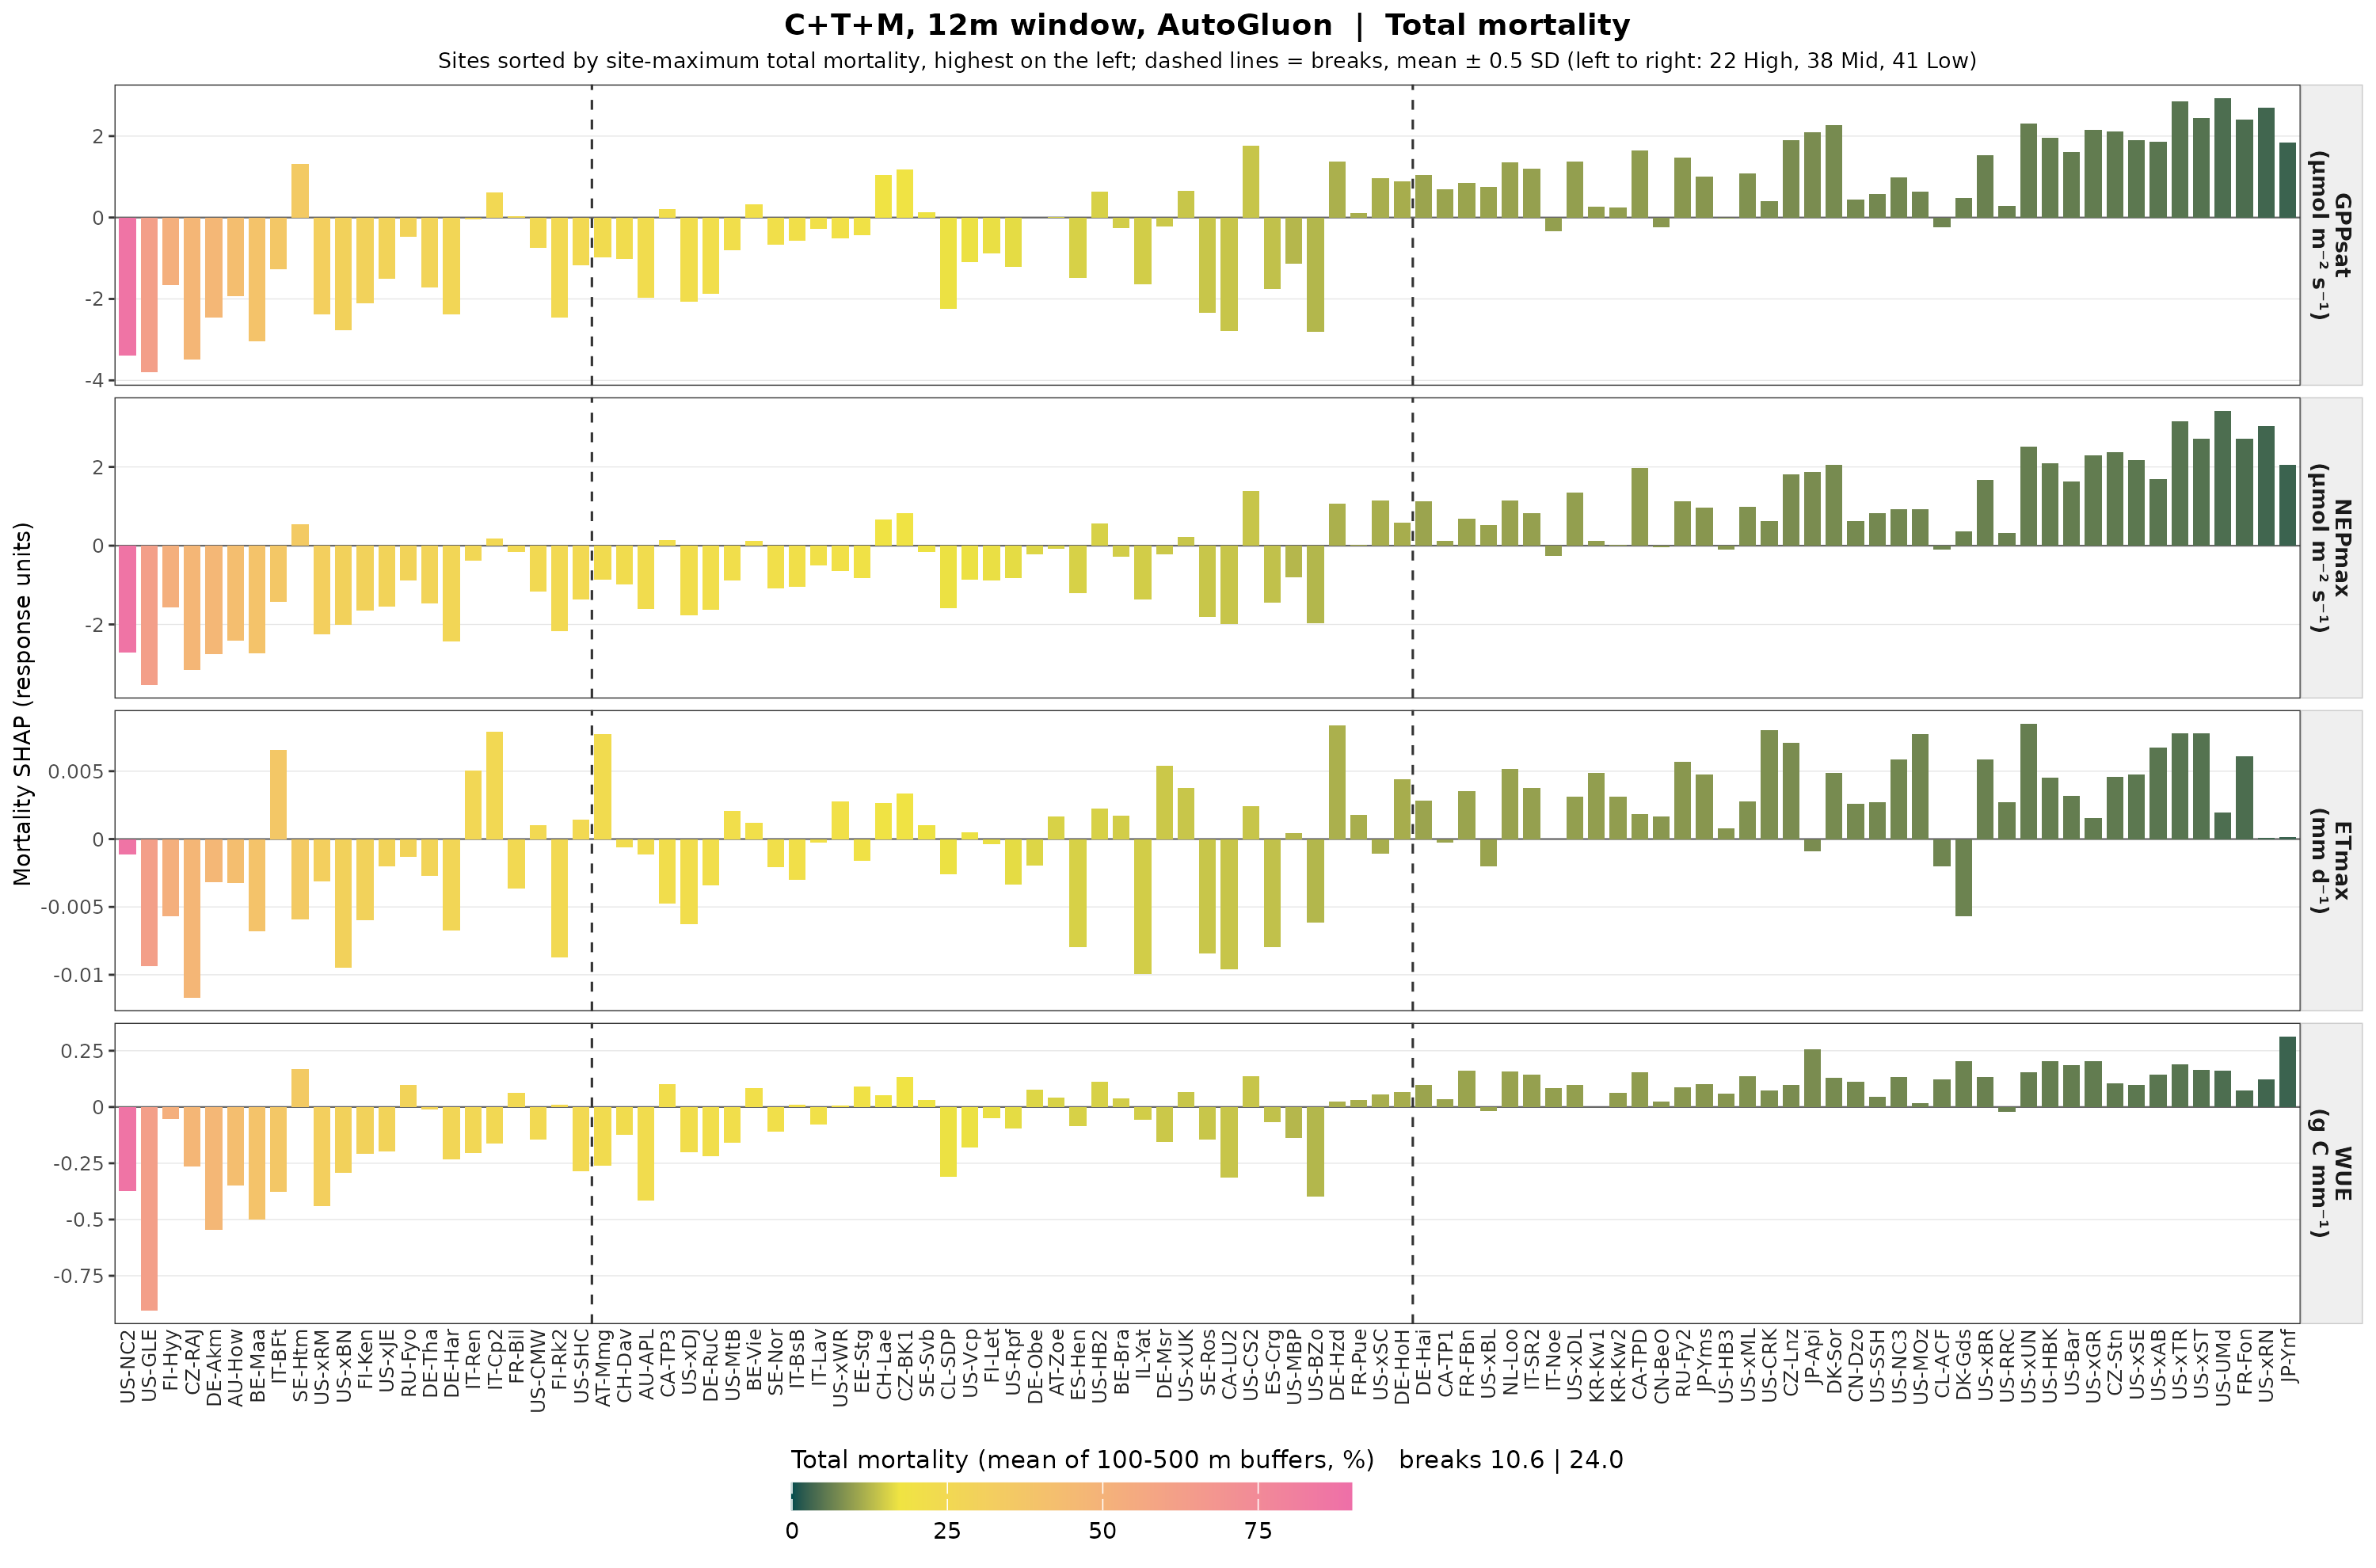
\includegraphics[width=\linewidth]{figures/A_fig3_signed_12m_AG.png}\\[2pt]
{\small \textbf{Fig.\ A4} --- Fig.~3 with the 12-month window, AutoGluon.}
\end{sidewaysfigure}
\begin{sidewaysfigure}
\centering
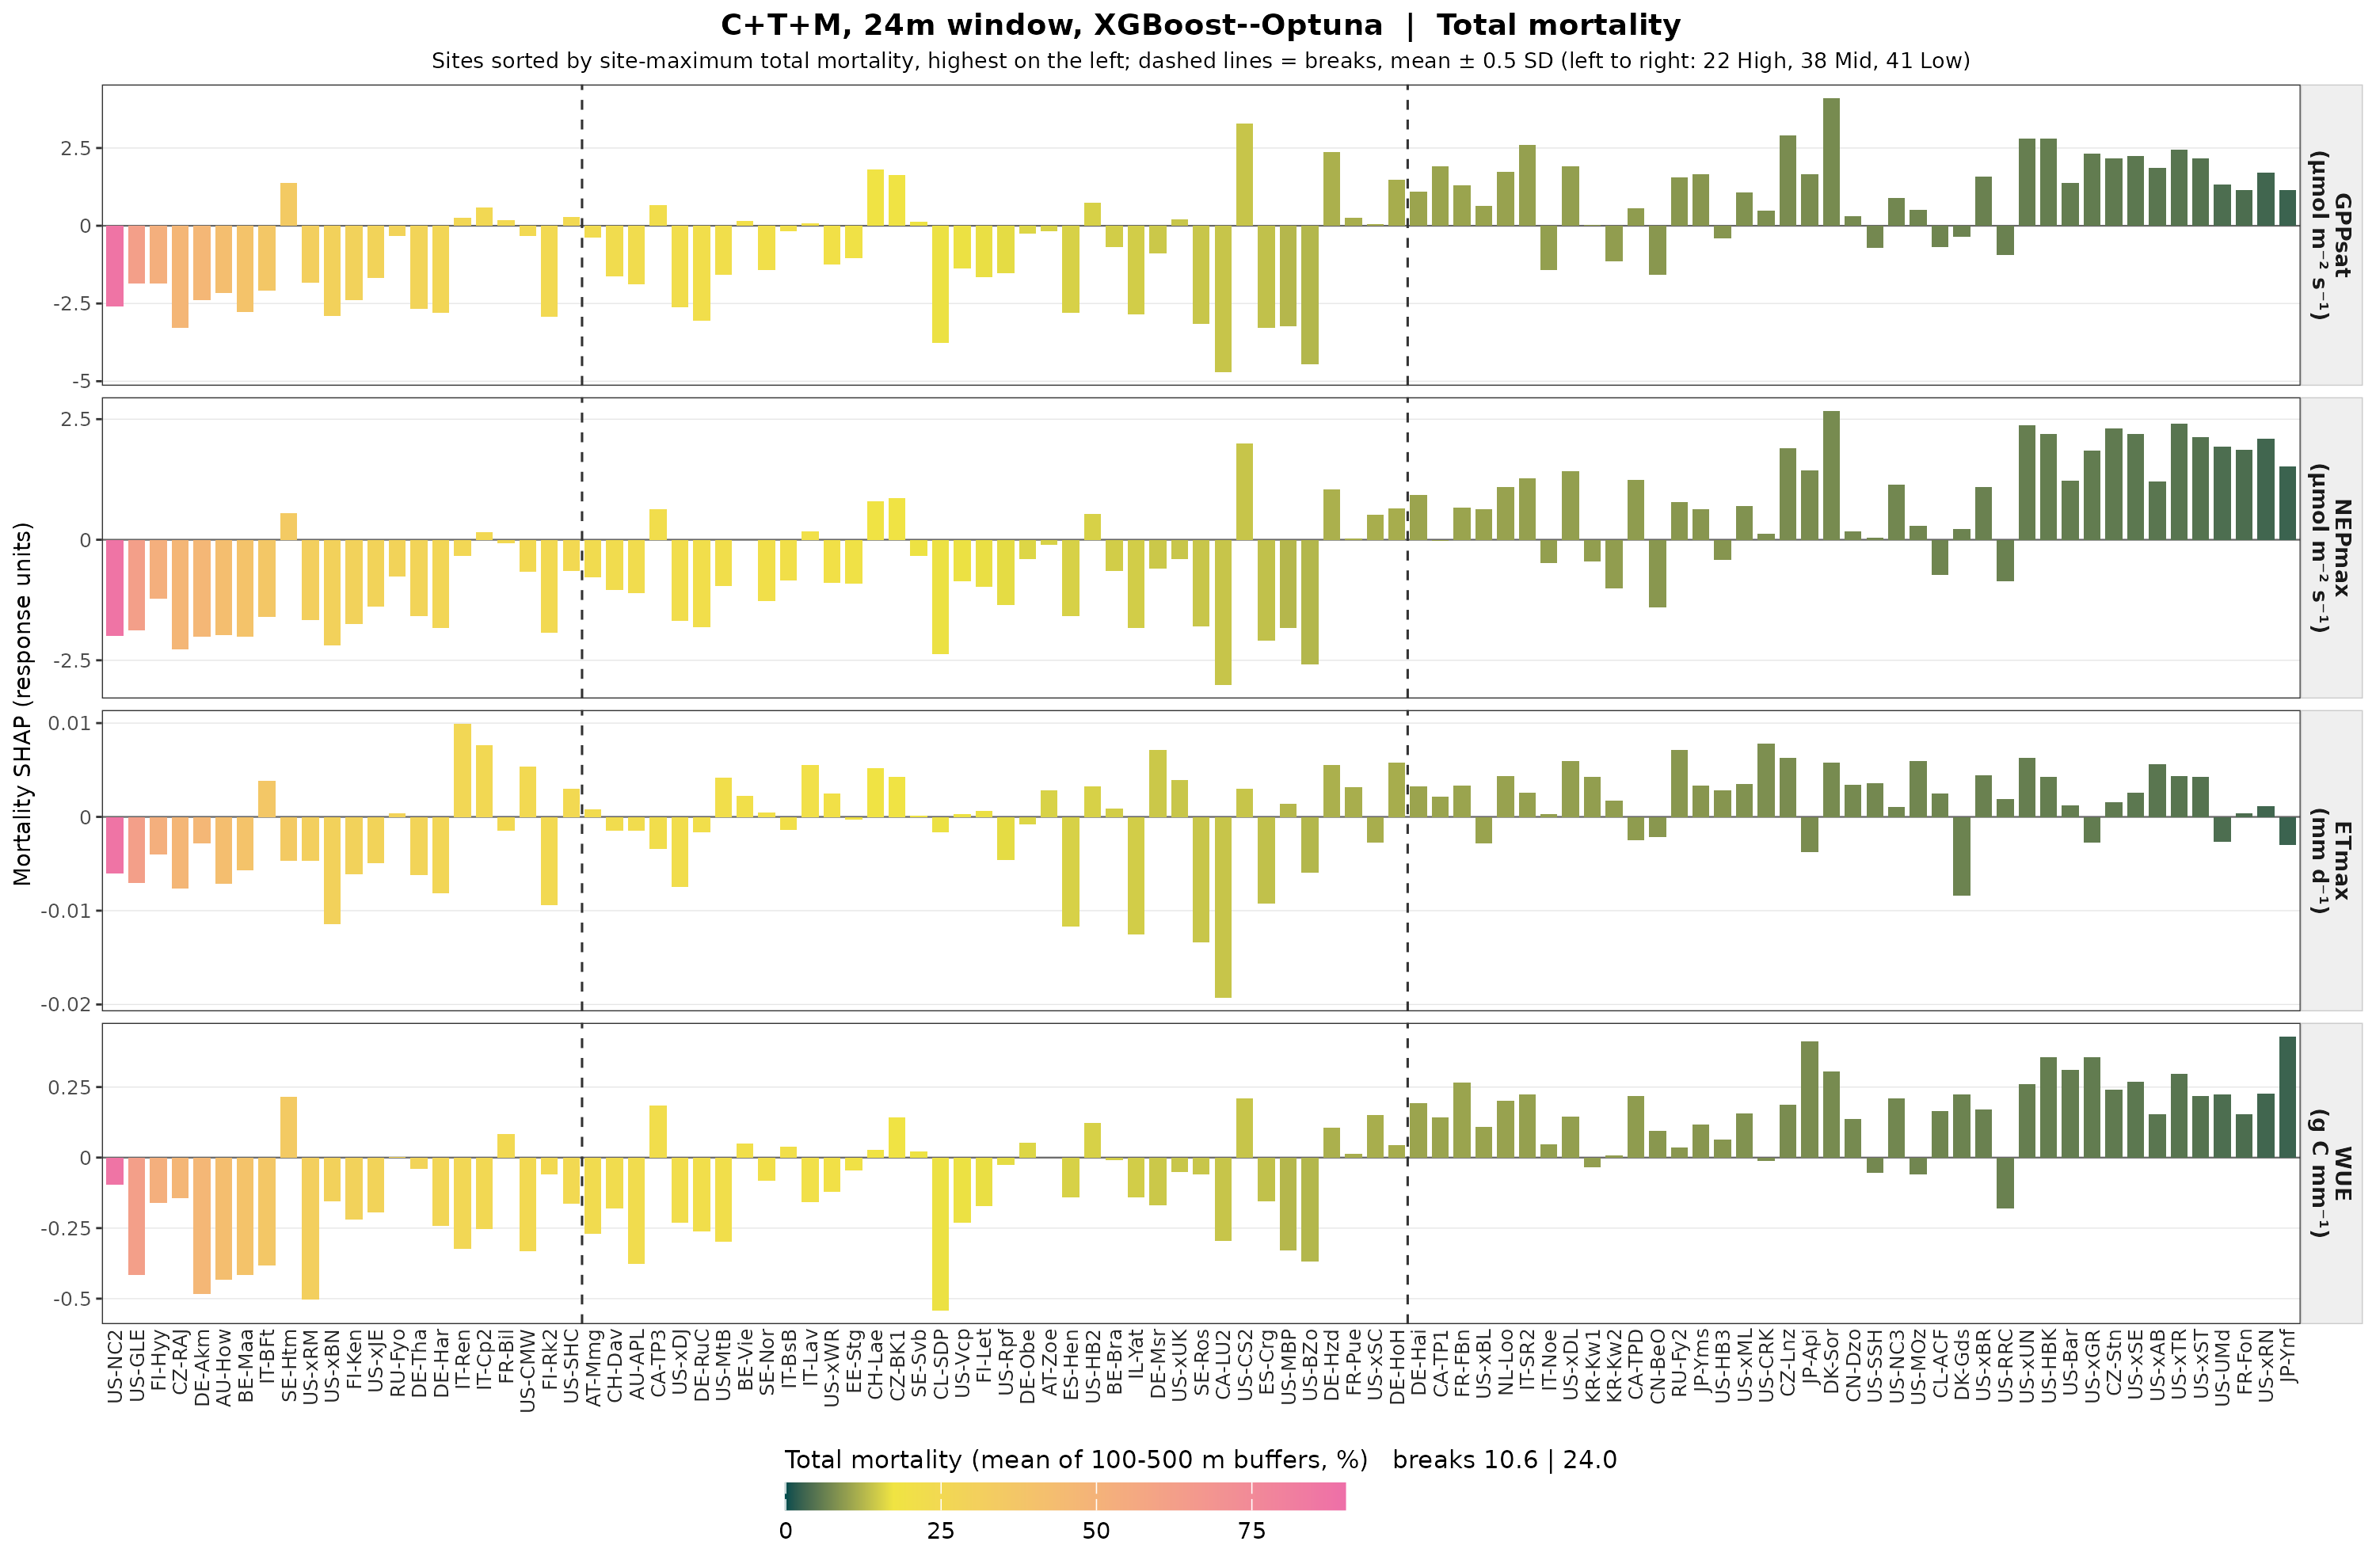
\includegraphics[width=\linewidth]{figures/A_fig3_signed_24m_XGB.png}\\[2pt]
{\small \textbf{Fig.\ A5} --- Fig.~3, XGBoost--Optuna, 24\,m.}
\end{sidewaysfigure}
\begin{sidewaysfigure}
\centering
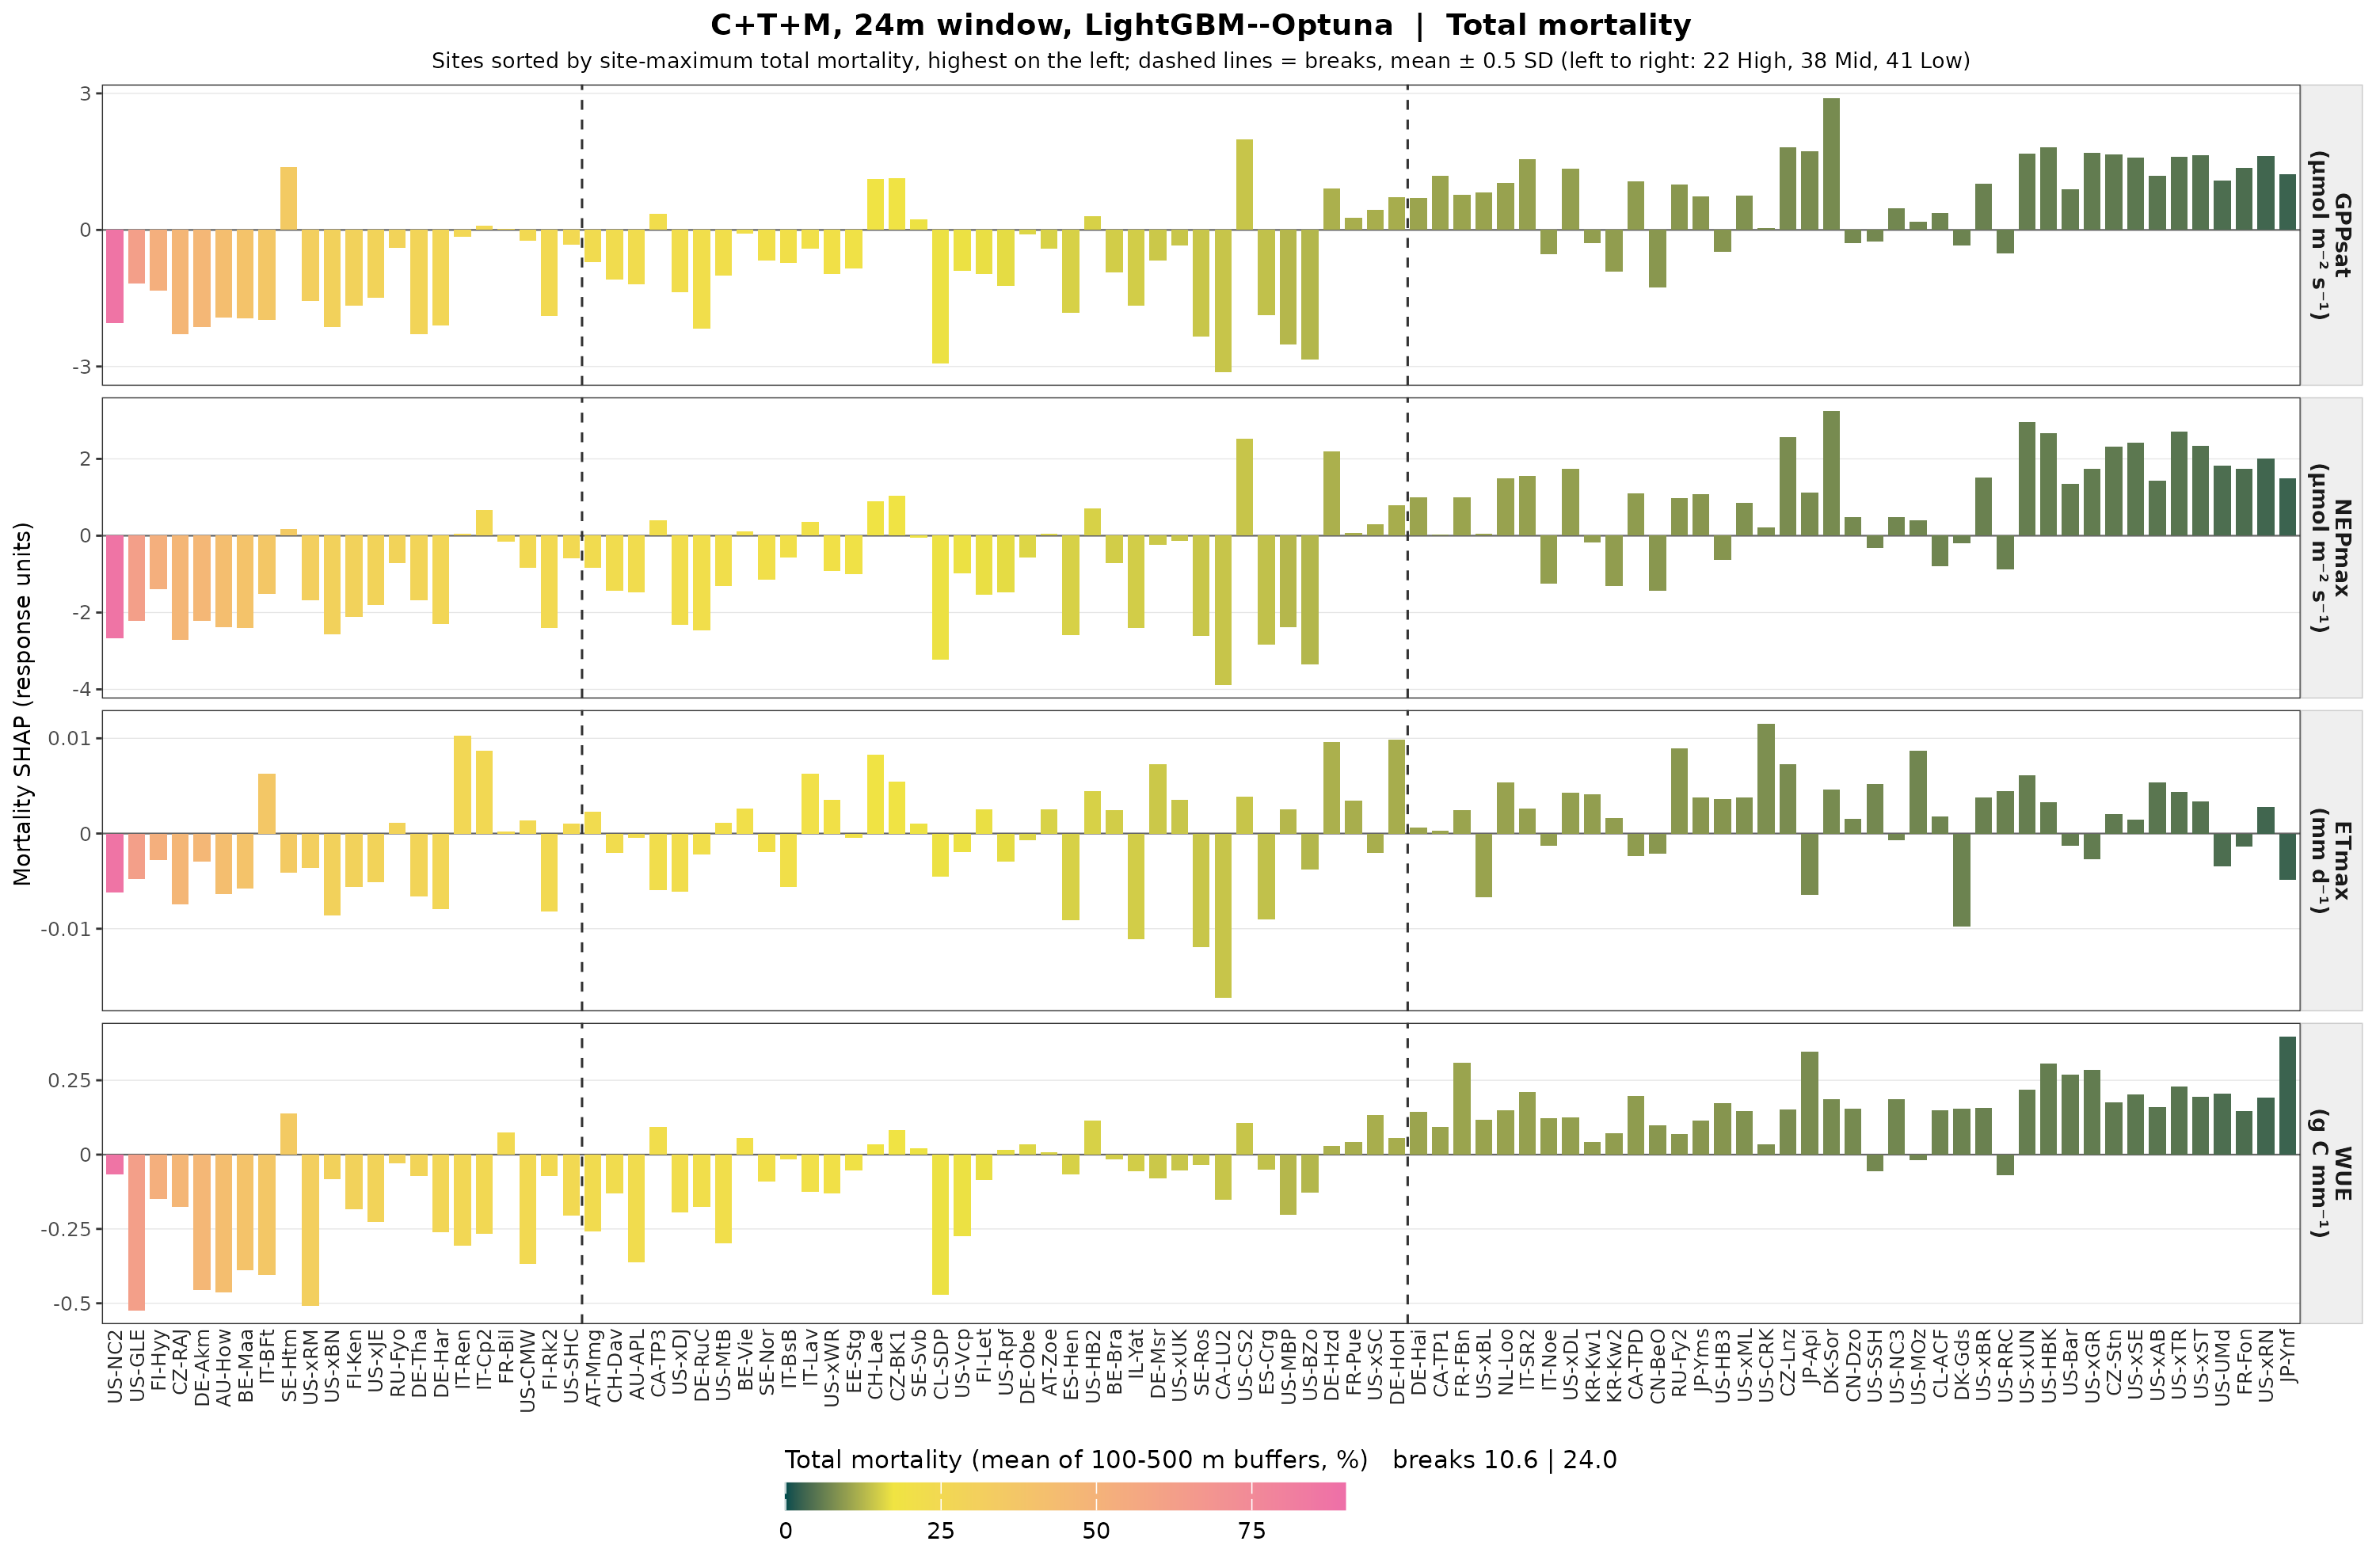
\includegraphics[width=\linewidth]{figures/A_fig3_signed_24m_LGB.png}\\[2pt]
{\small \textbf{Fig.\ A6} --- Fig.~3, LightGBM--Optuna, 24\,m.}
\end{sidewaysfigure}

\clearpage
\subsection*{A4. Figure 4: all learners and relative deadwood}
\begin{center}
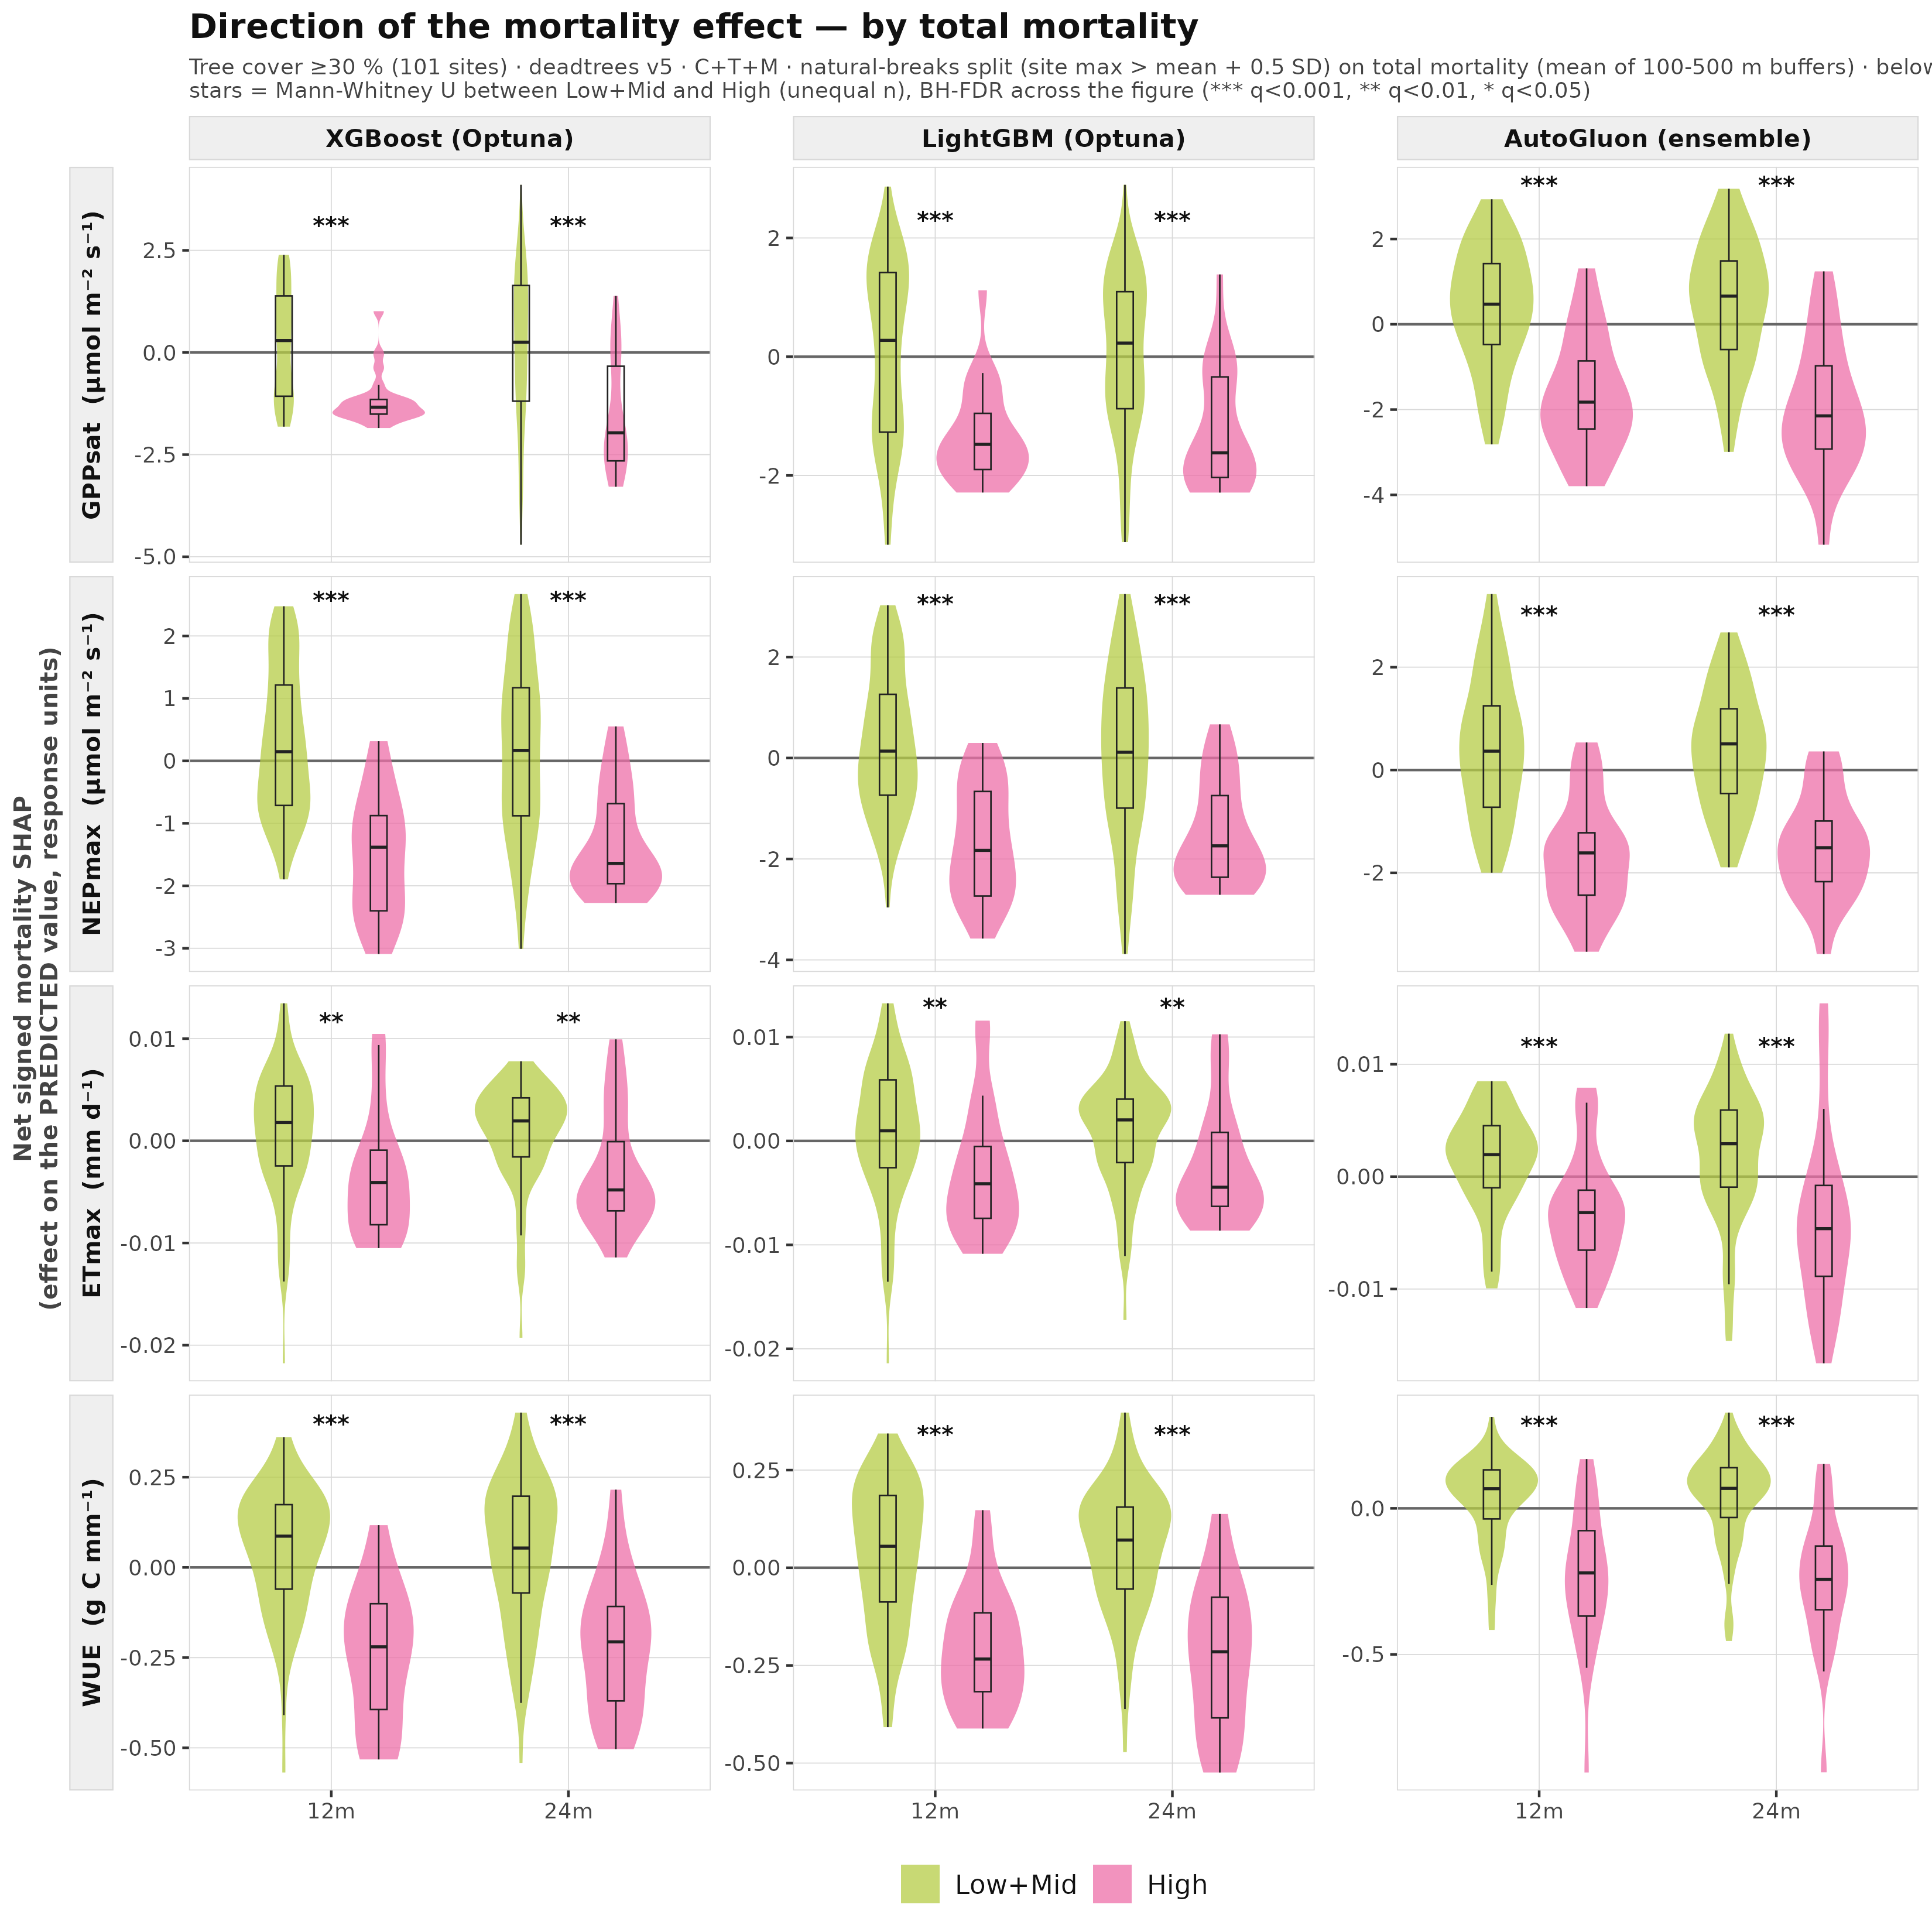
\includegraphics[width=0.85\linewidth]{figures/A_fig4_total_mort_all_learners.png}\\[2pt]
{\small \textbf{Fig.\ A7} --- Fig.~4 for all three learners (total mortality).}
\end{center}
\begin{center}
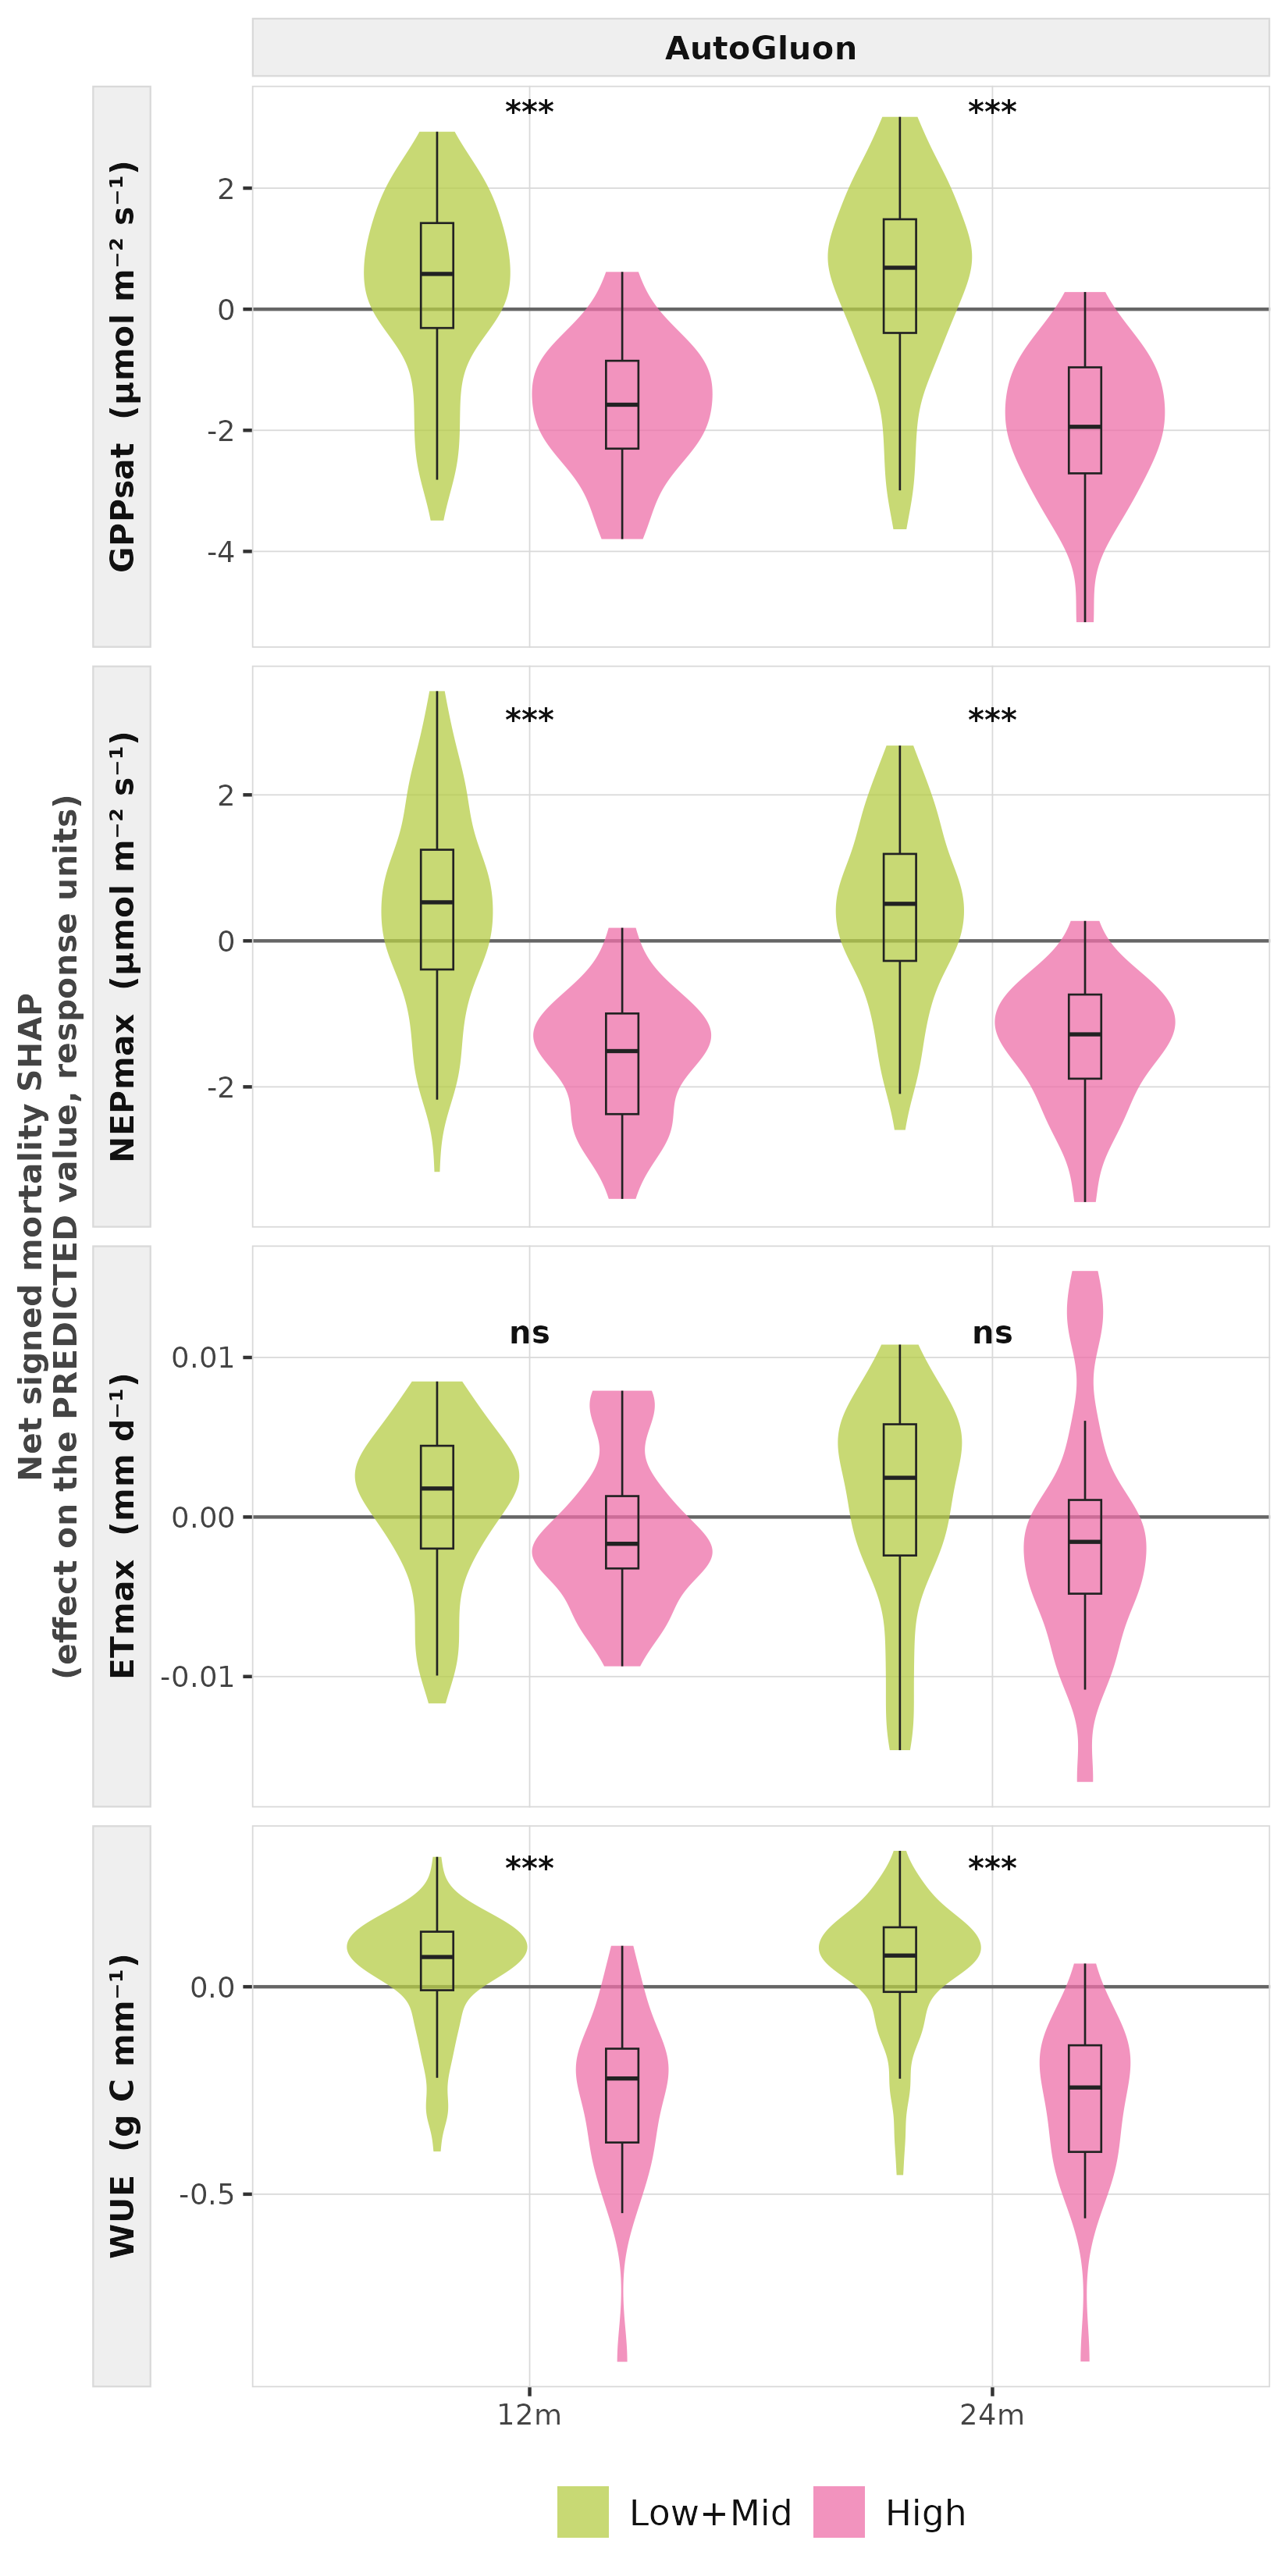
\includegraphics[width=0.48\linewidth]{figures/A_fig4_rel_deadwood_AG.png}\\[2pt]
{\small \textbf{Fig.\ A8} --- Fig.~4 split by relative deadwood, AutoGluon.}
\end{center}

\subsection*{A5. Mortality block: drop-column test and the tree learners}
\begin{center}
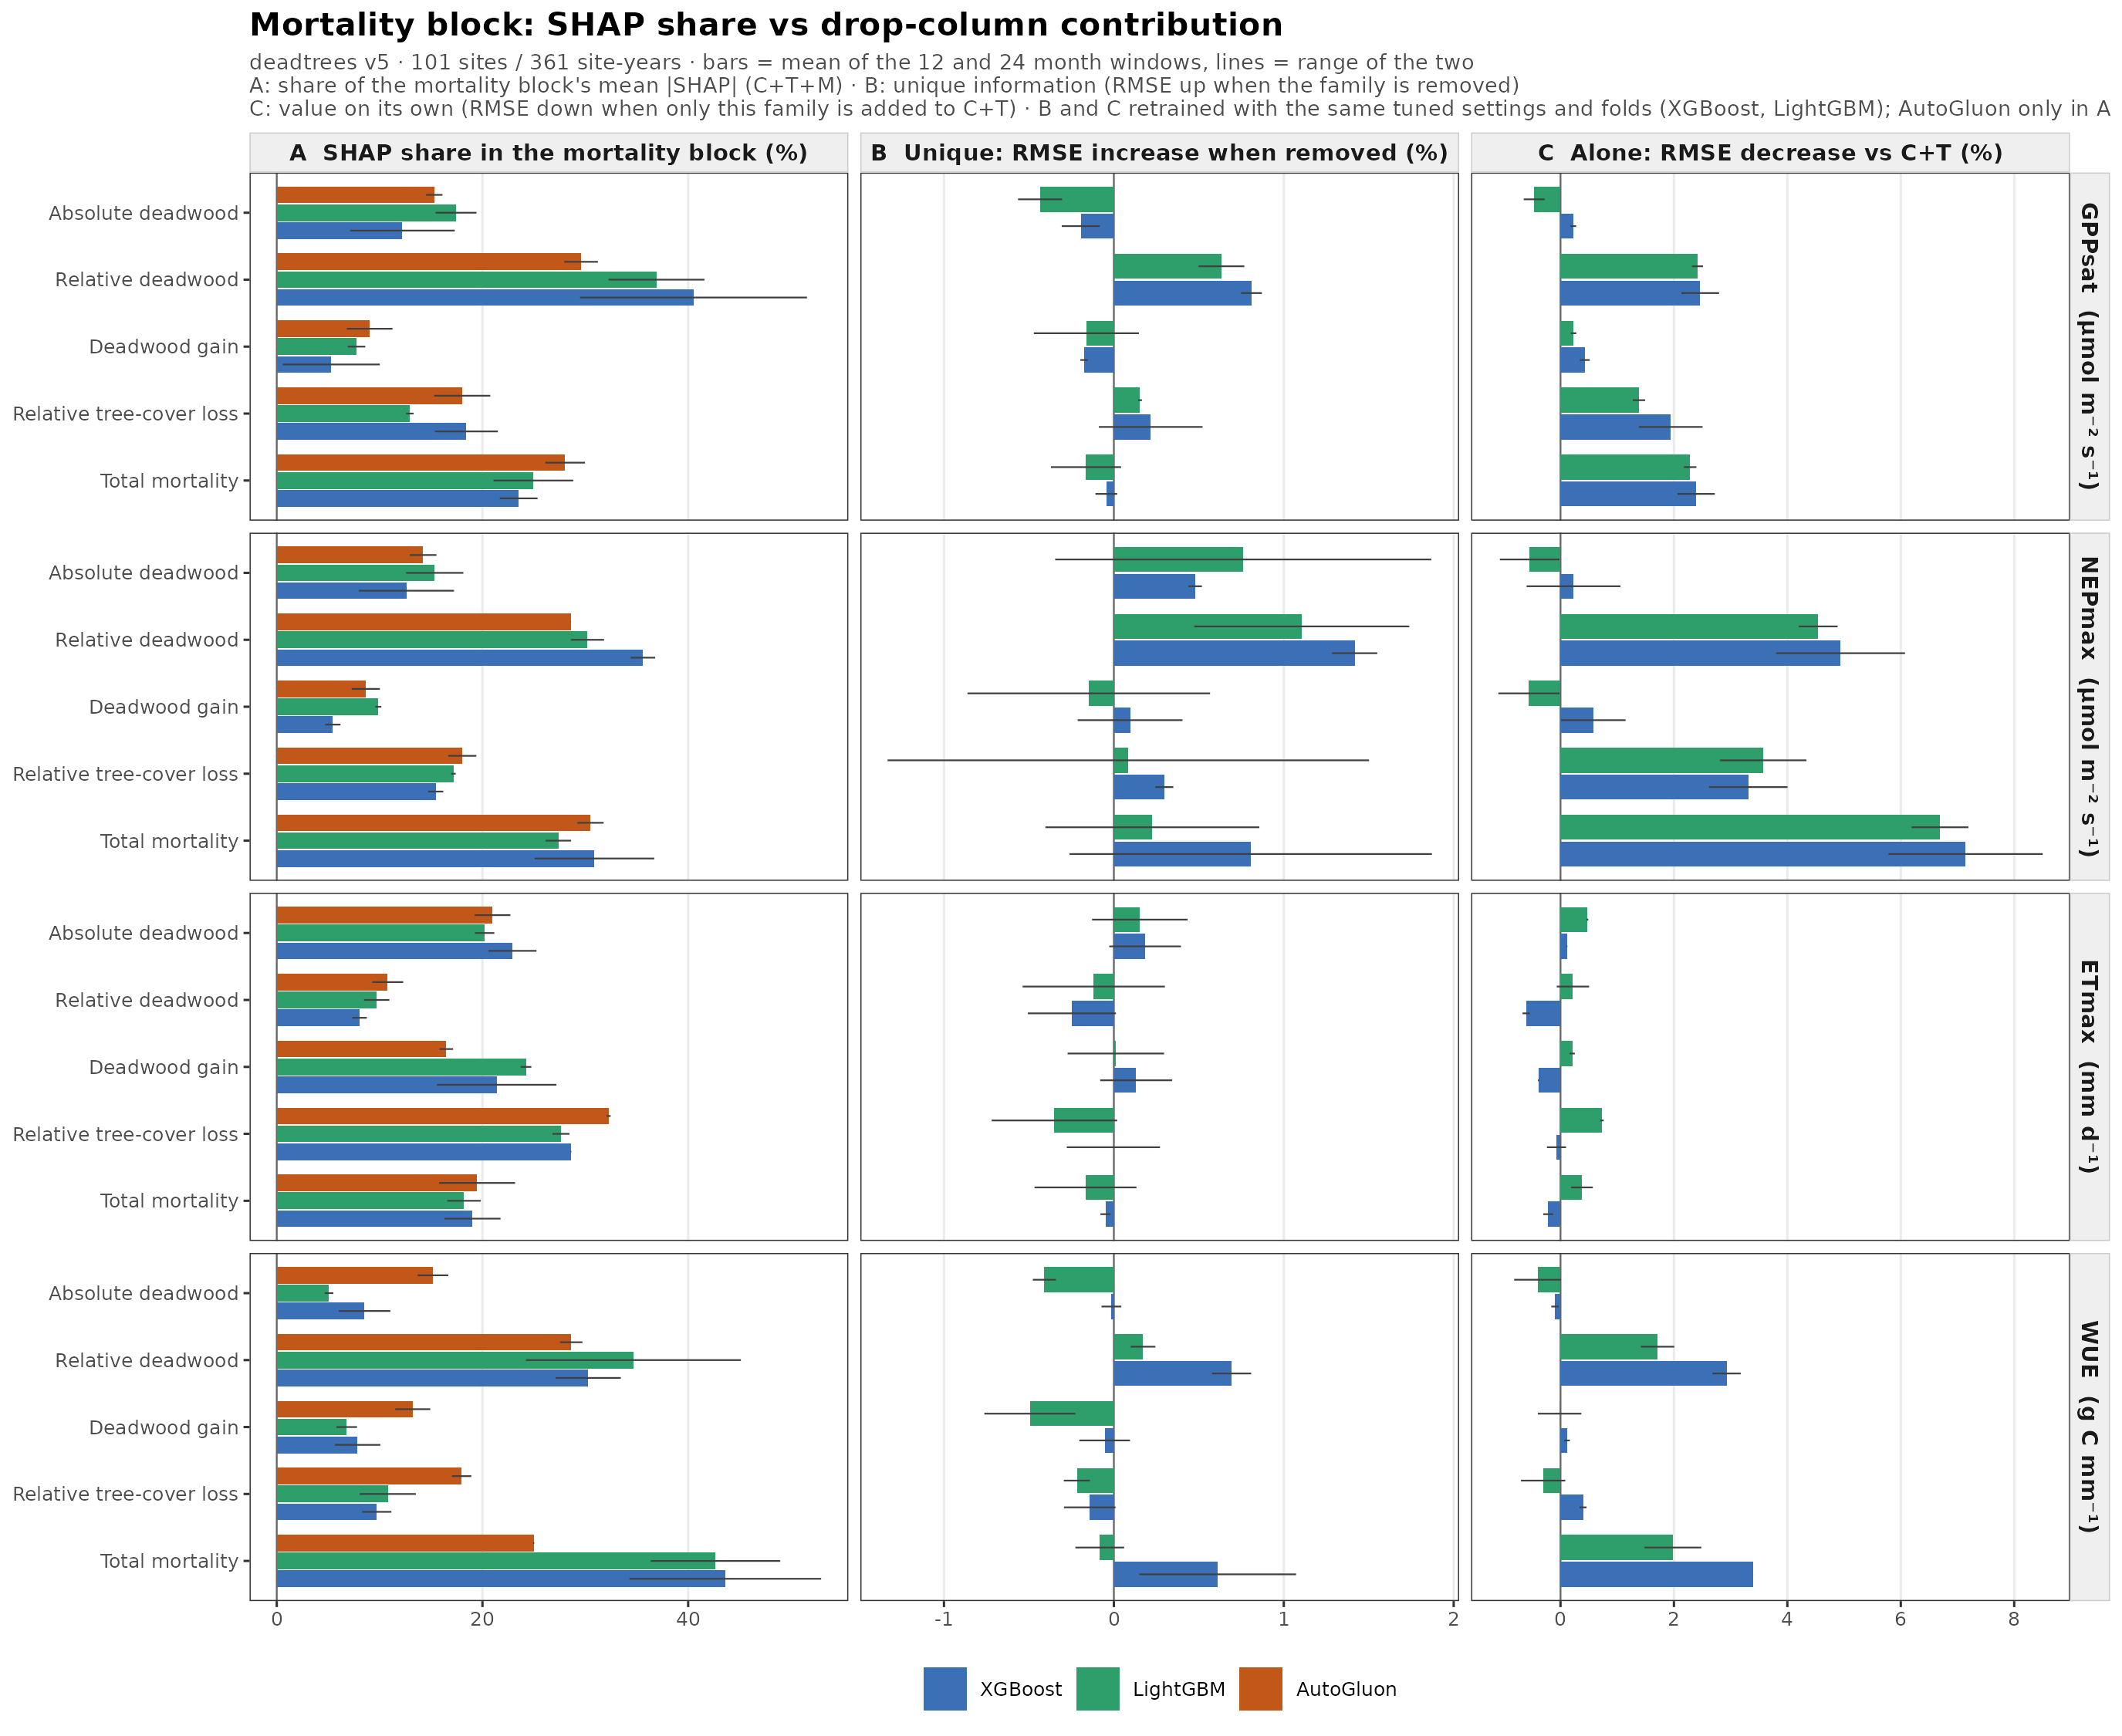
\includegraphics[width=\linewidth]{figures/A_fig6_dropcol.png}\\[2pt]
{\small \textbf{Fig.\ A9} --- per metric: A SHAP share in the mortality block (all learners); B RMSE increase when the
metric is removed from C+T+M; C RMSE decrease when only this metric is added to C+T (B and C: XGBoost and LightGBM retrained
with the same tuned settings and folds).}
\end{center}
\begin{center}
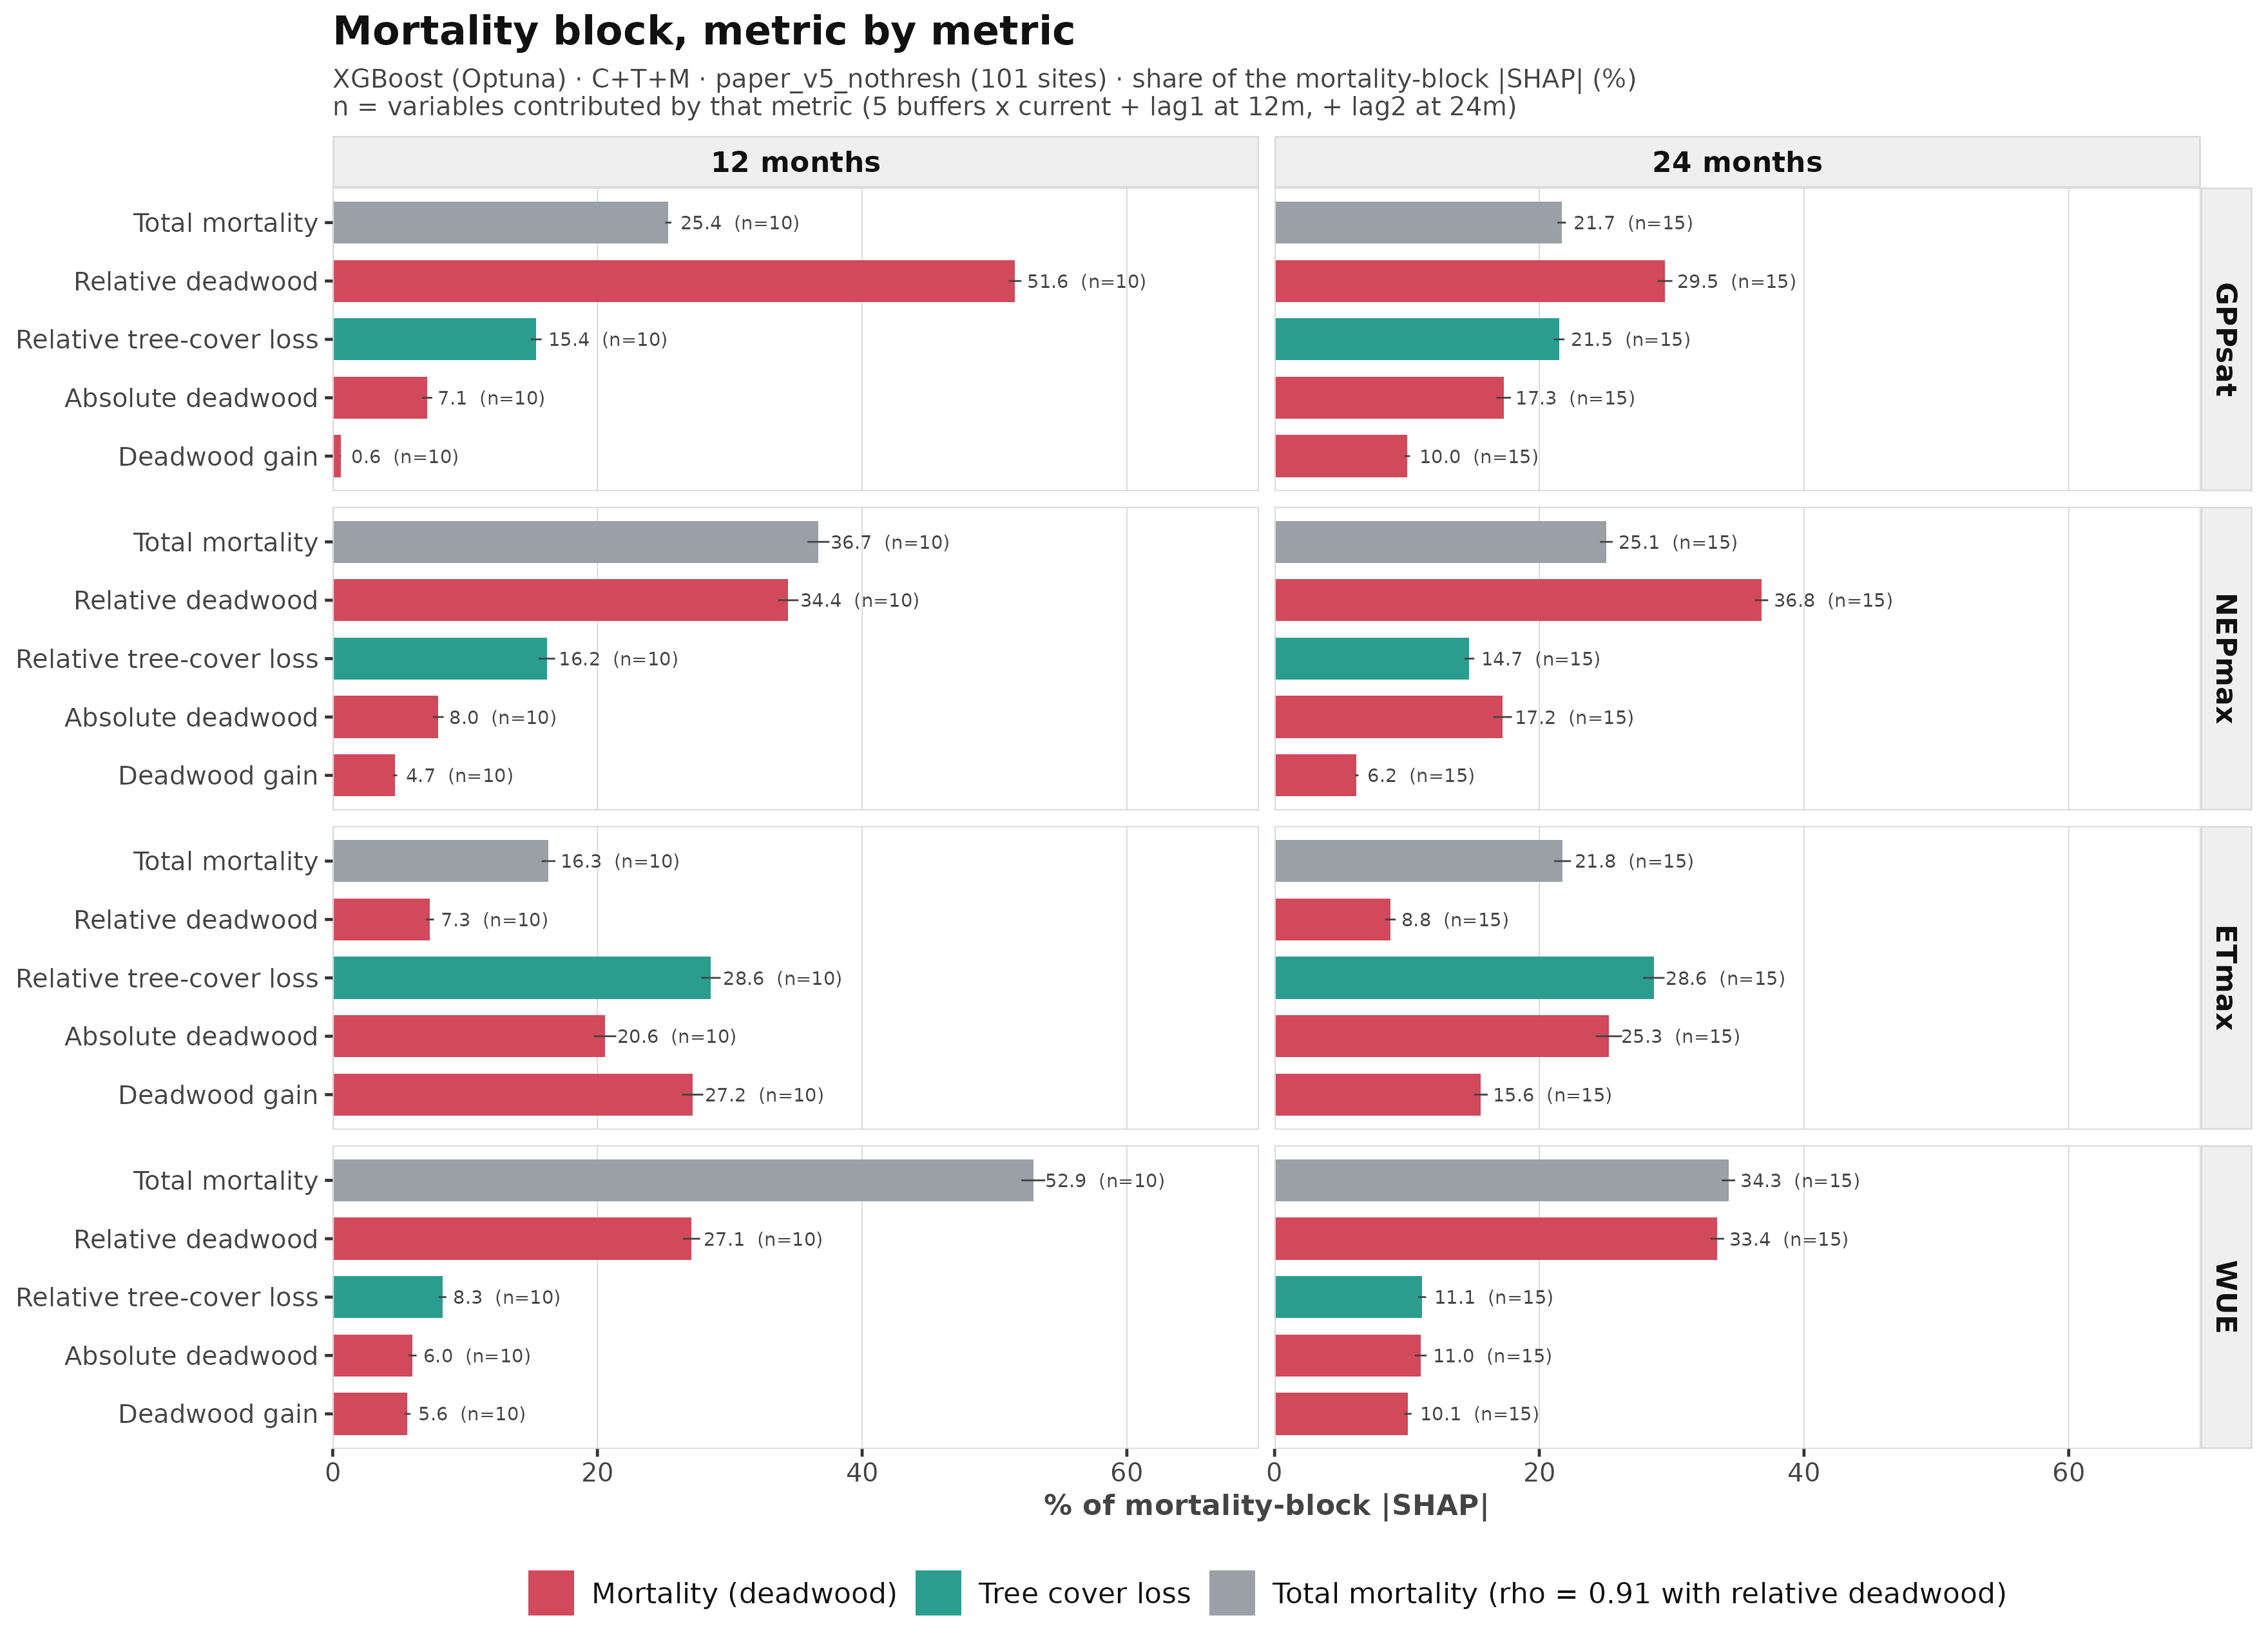
\includegraphics[width=0.8\linewidth]{figures/A_fig6_mortality_block_XGB.png}\\[2pt]
{\small \textbf{Fig.\ A10} --- Fig.~6 for XGBoost.}
\end{center}
\begin{center}
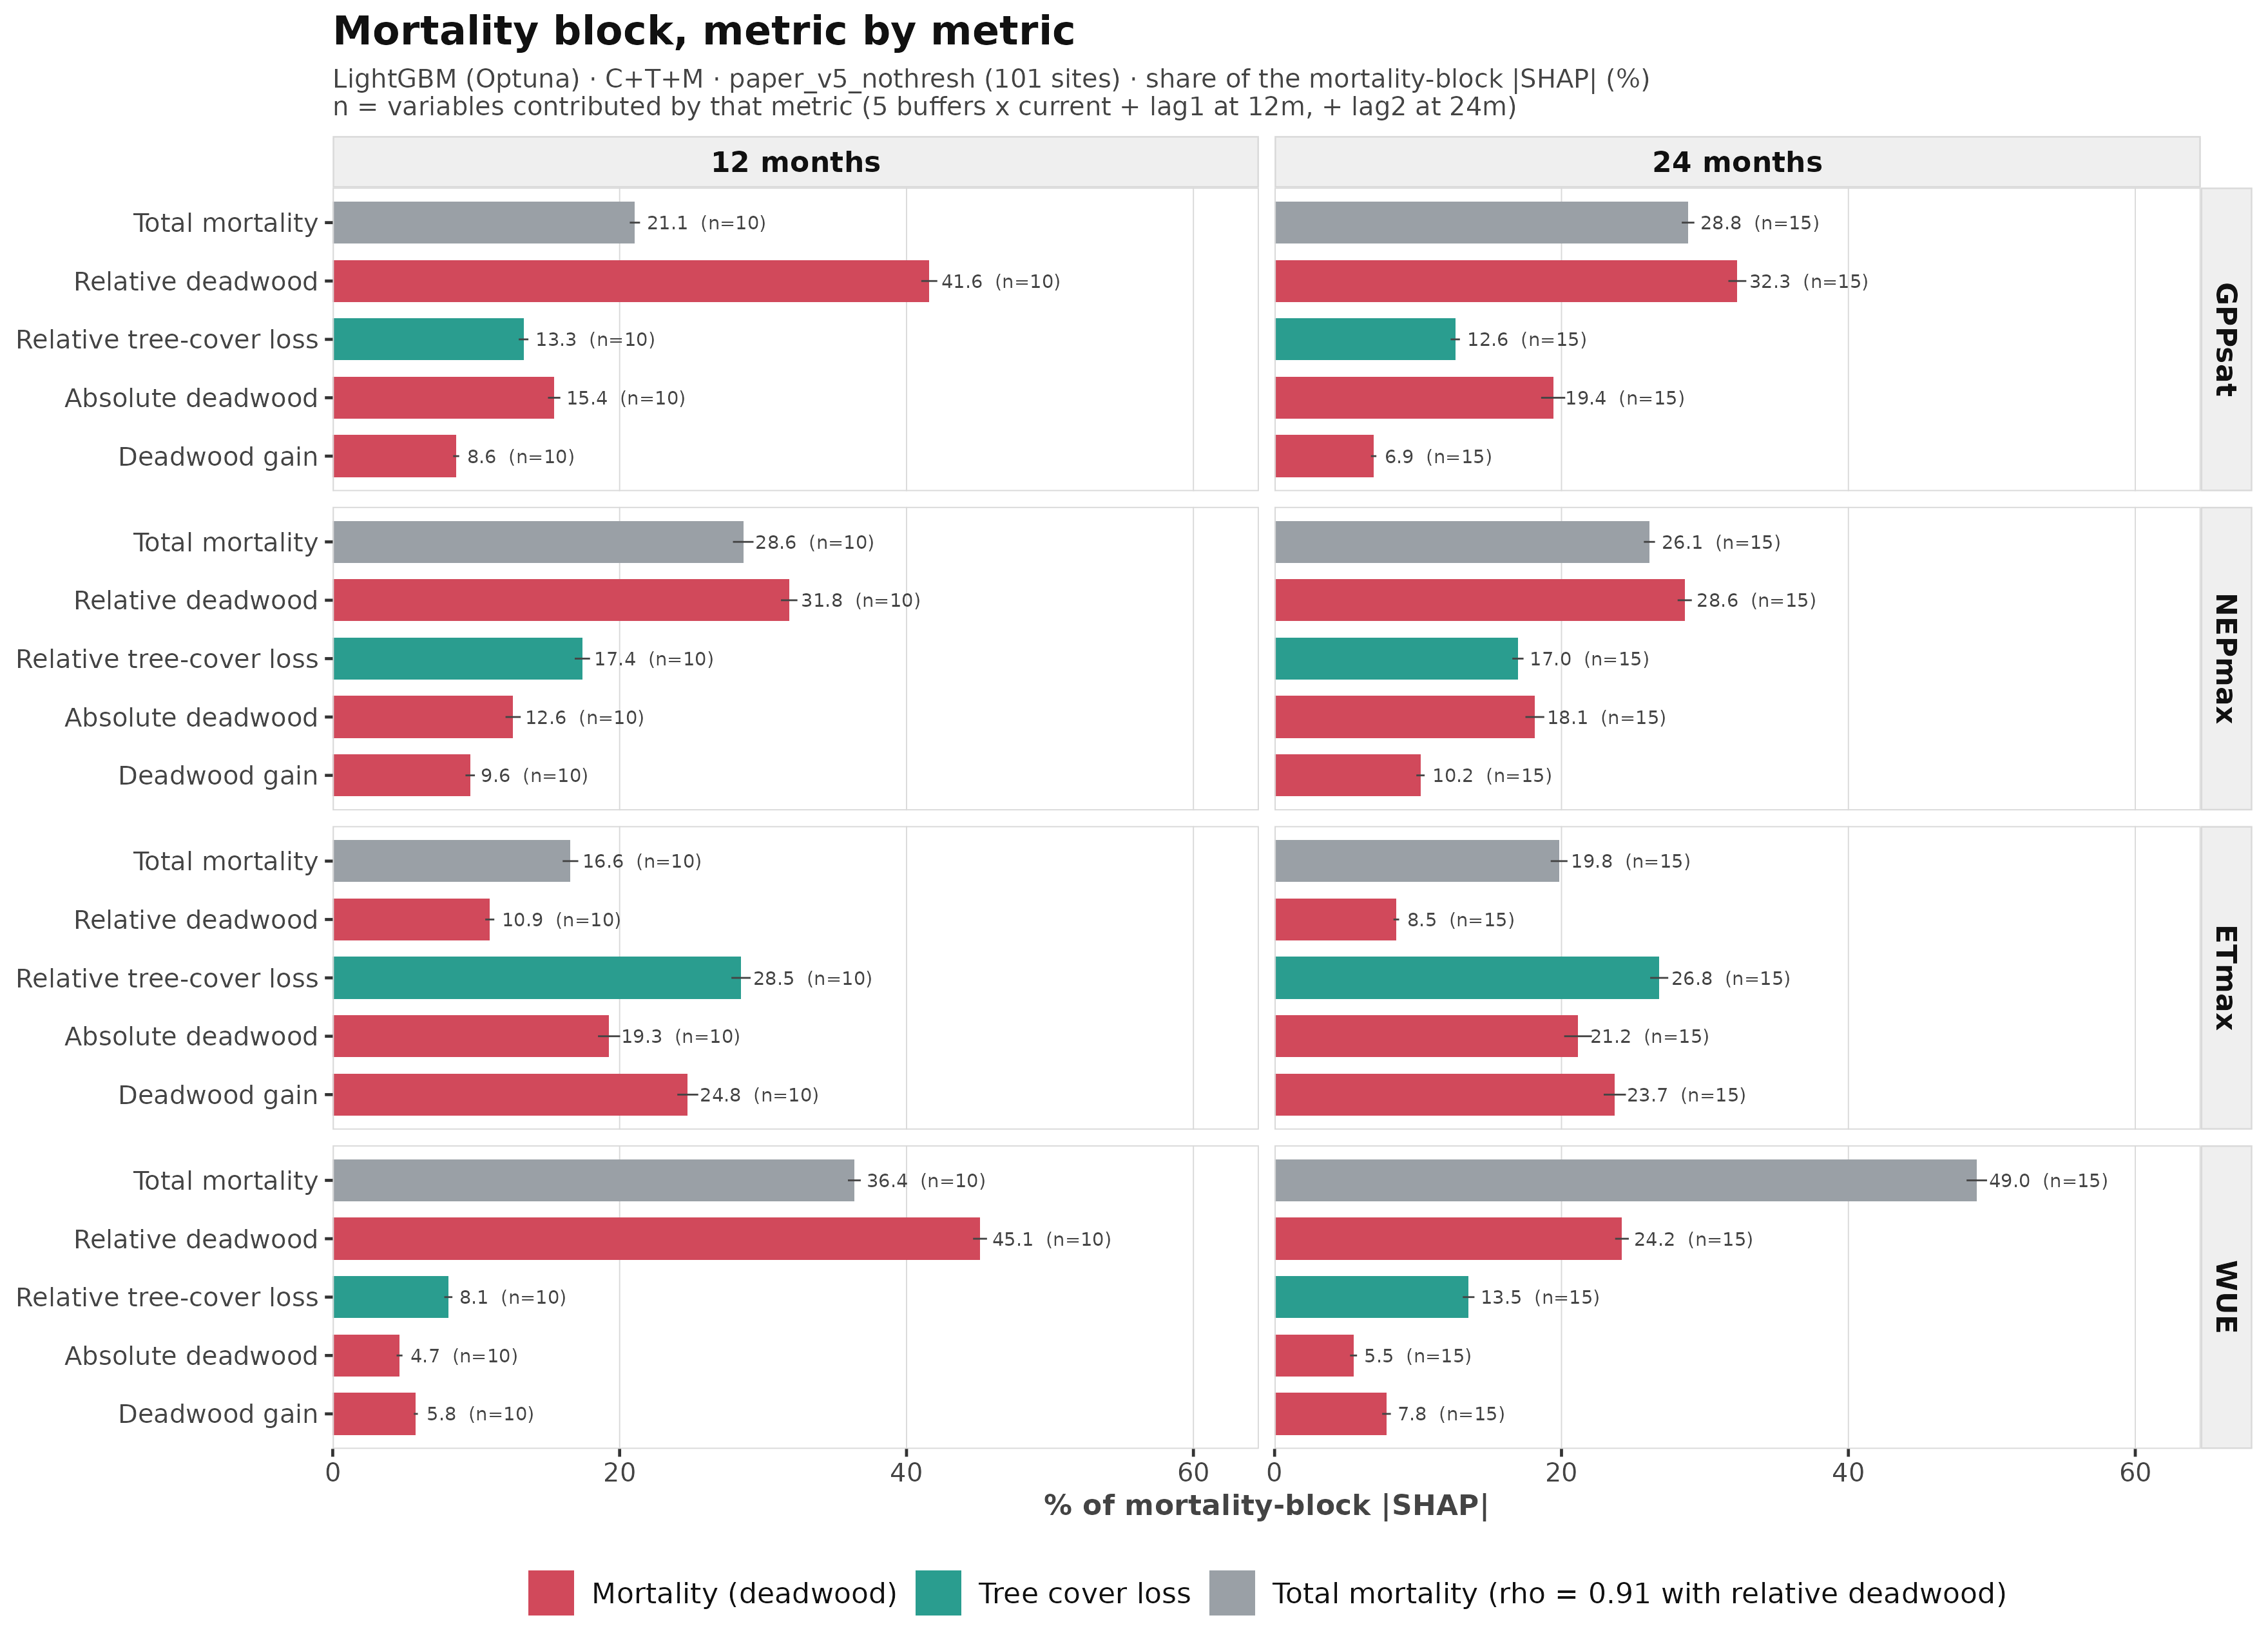
\includegraphics[width=0.8\linewidth]{figures/A_fig6_mortality_block_LGB.png}\\[2pt]
{\small \textbf{Fig.\ A11} --- Fig.~6 for LightGBM.}
\end{center}

\subsection*{A6. Figure 5: 12-month window and XGBoost}
\begin{center}
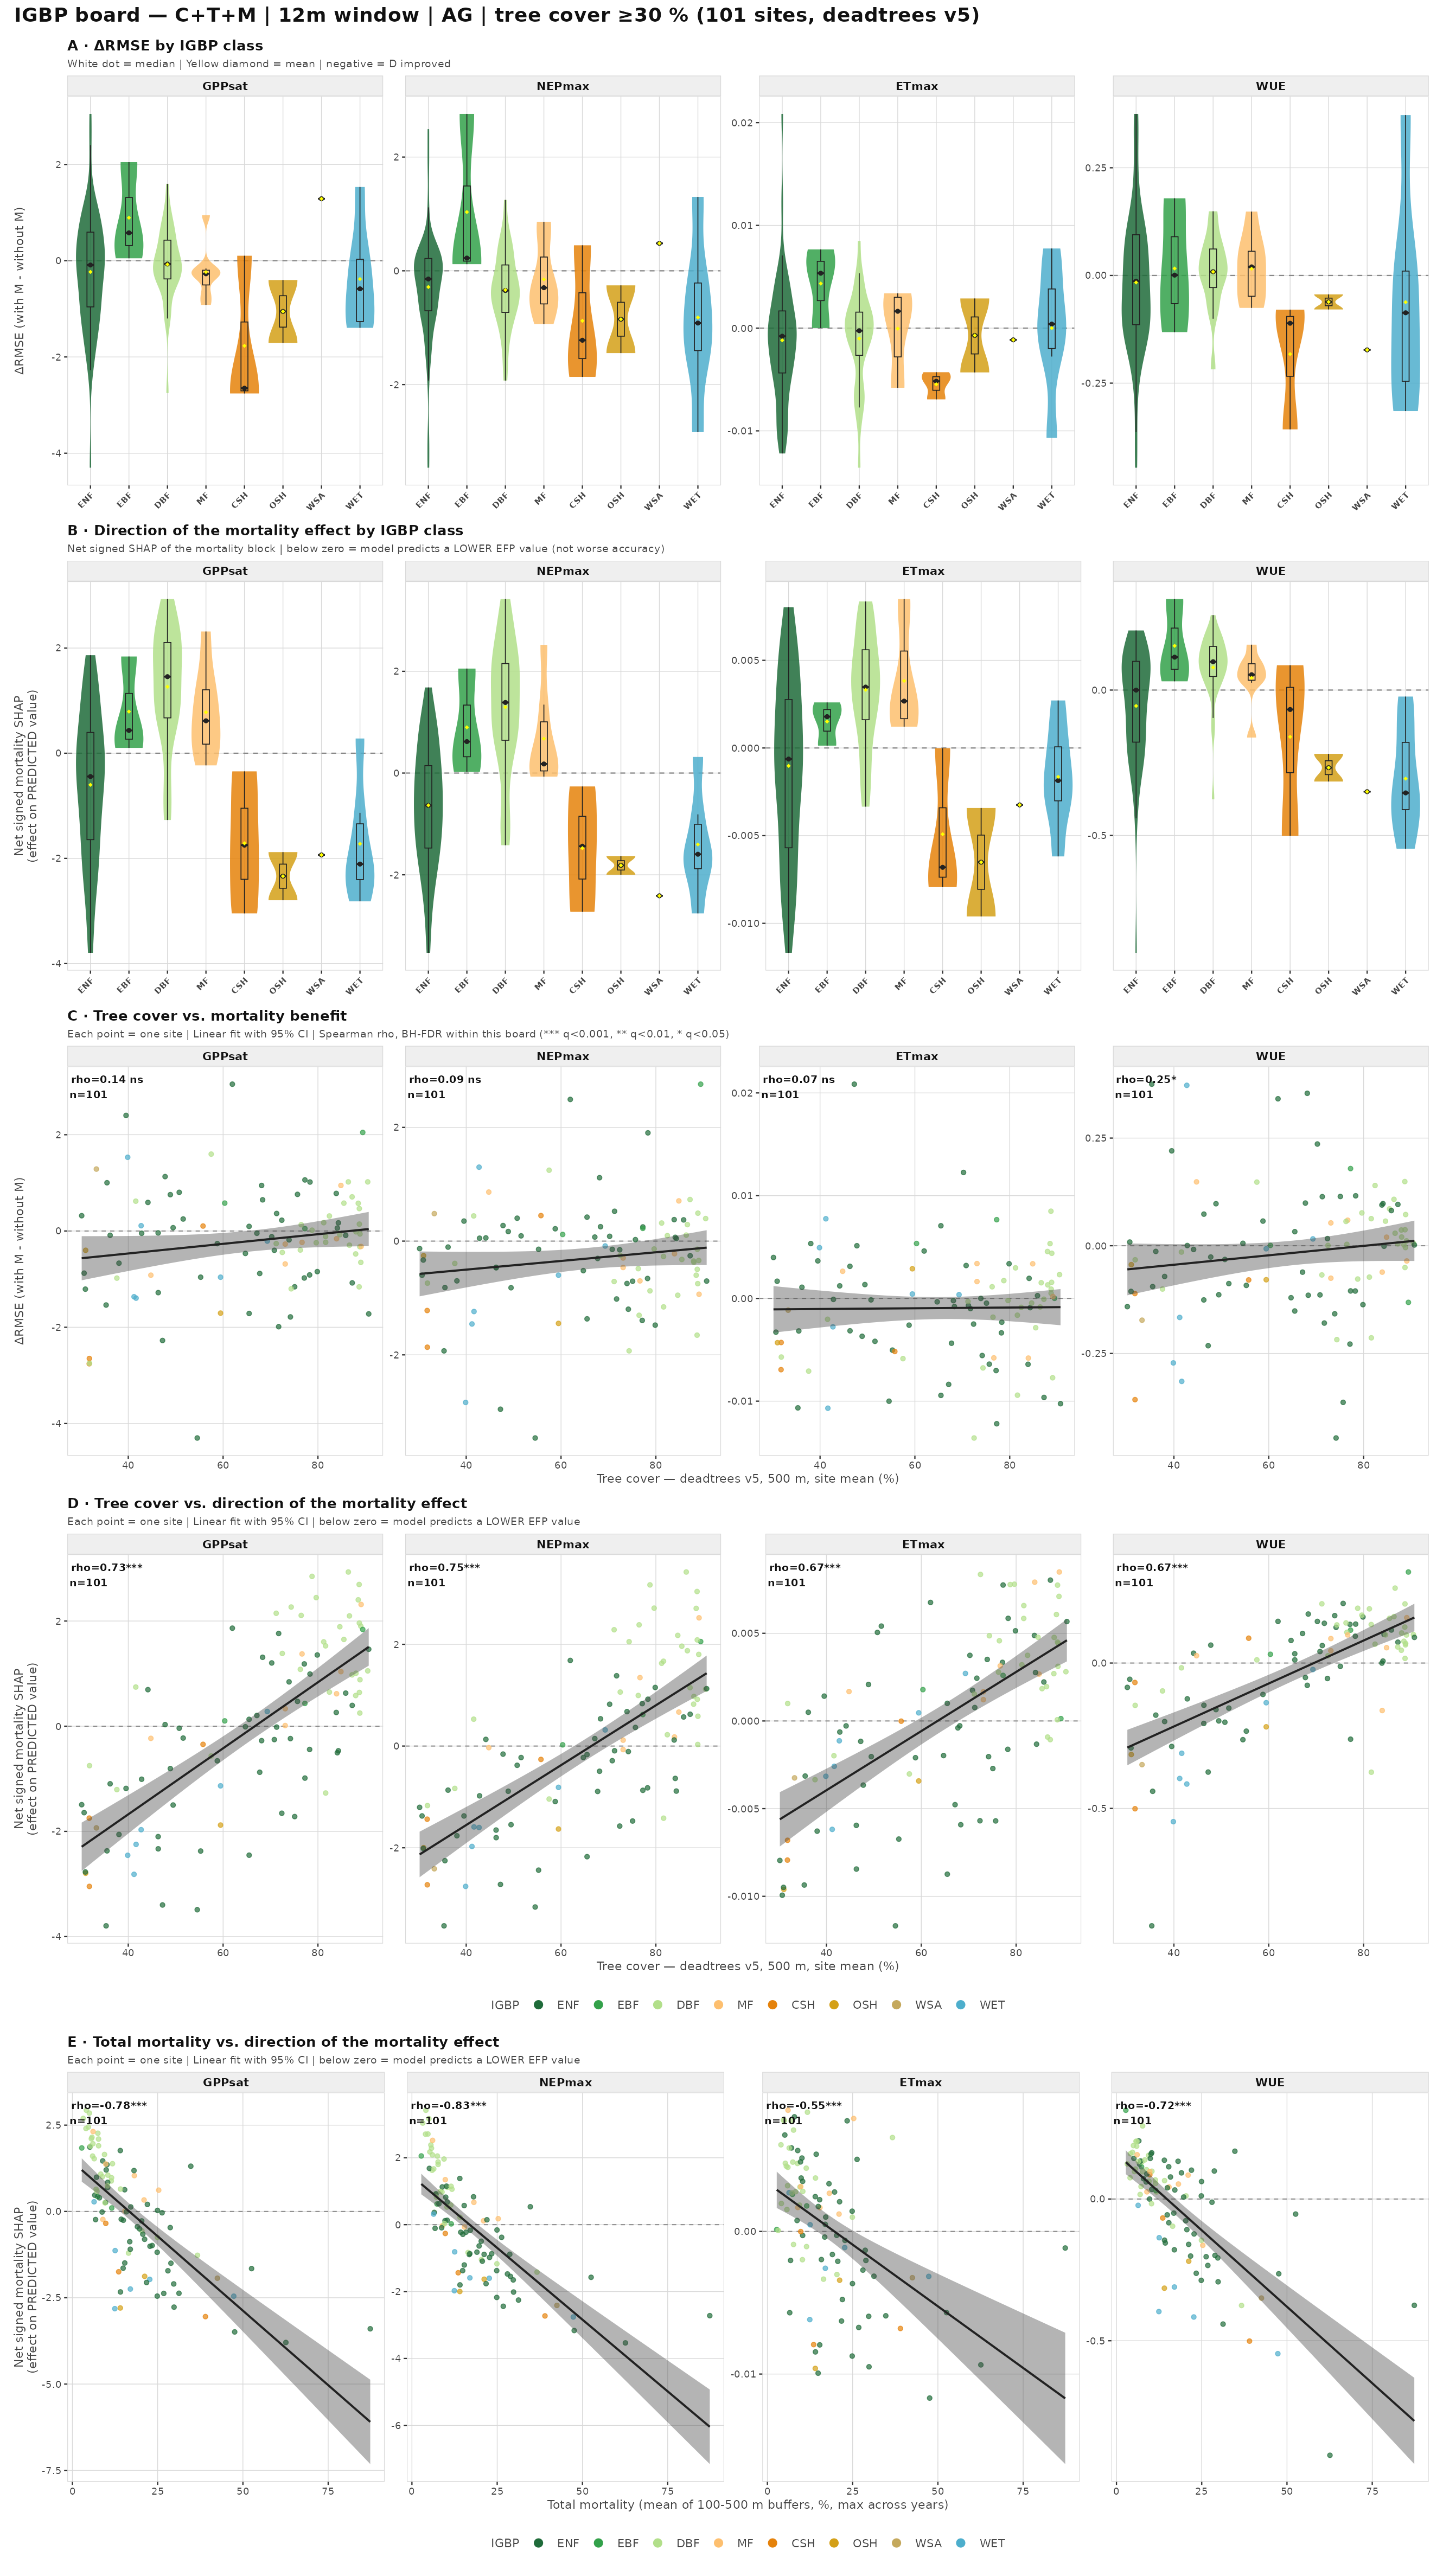
\includegraphics[width=0.82\linewidth]{figures/A_fig5_igbp_12m_AG.png}\\[2pt]
{\small \textbf{Fig.\ A12} --- Fig.~5 with the 12-month window, AutoGluon.}
\end{center}
\begin{center}
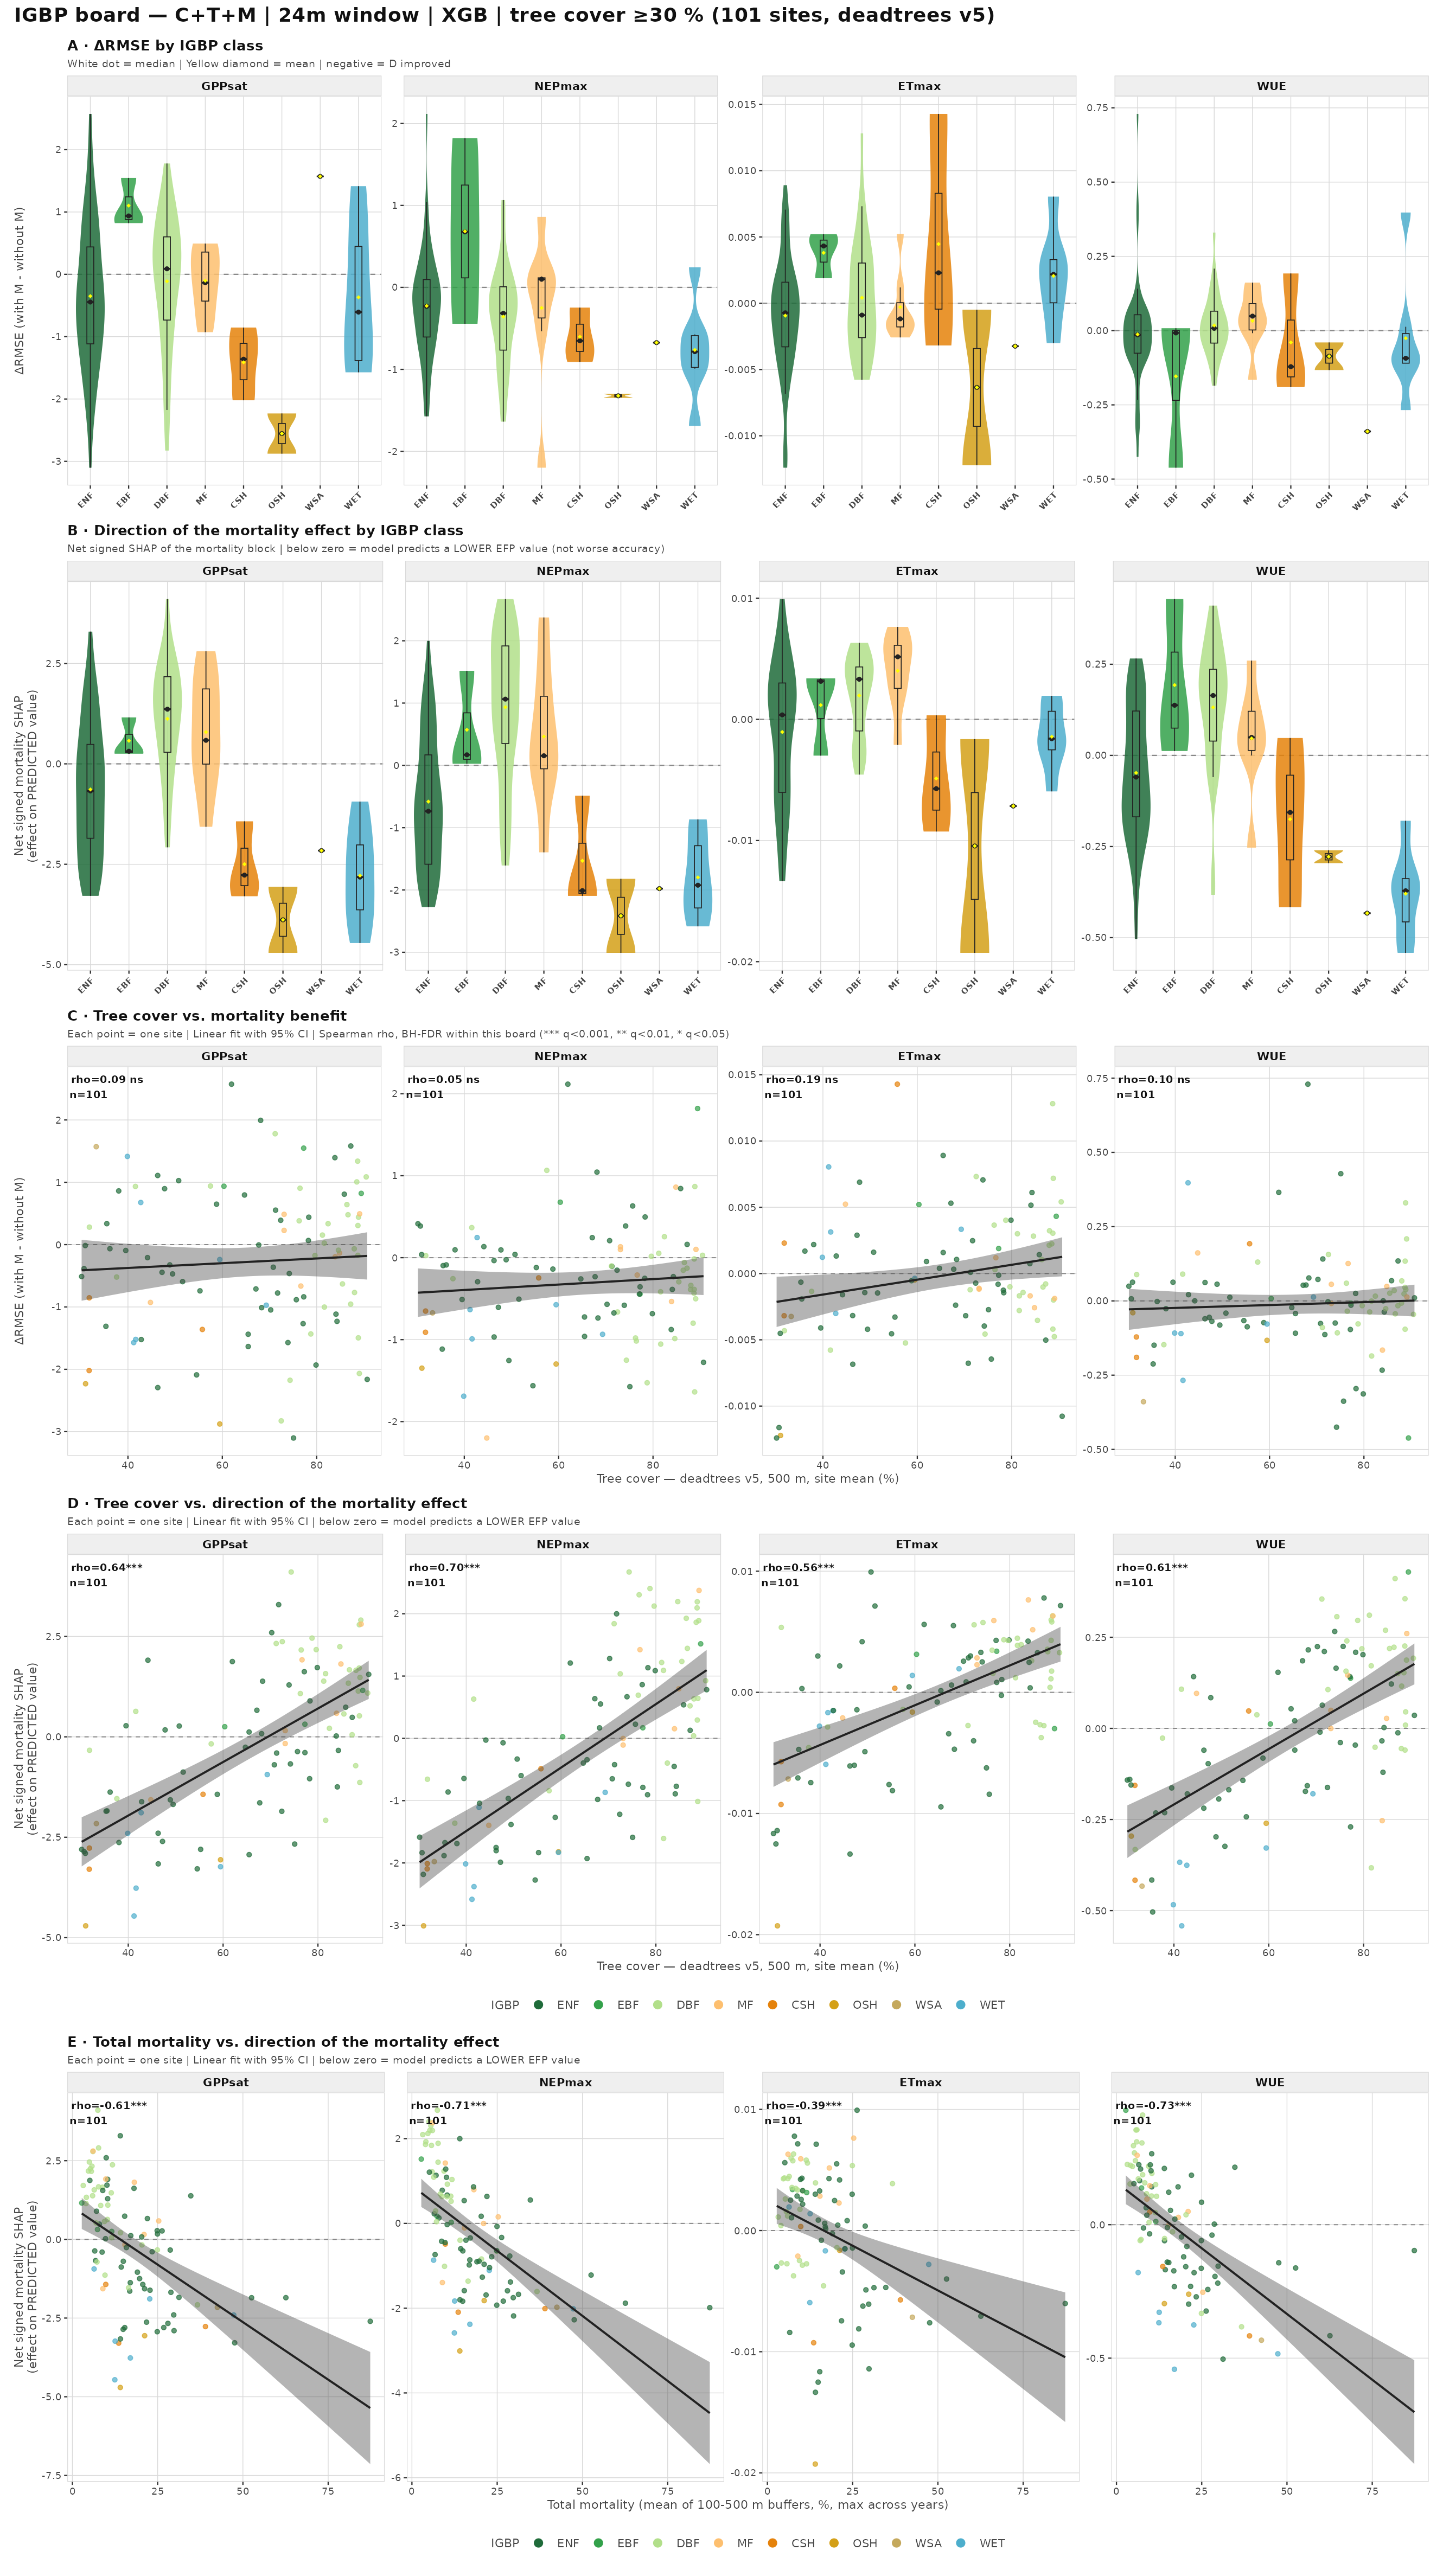
\includegraphics[width=0.82\linewidth]{figures/A_fig5_igbp_24m_XGB.png}\\[2pt]
{\small \textbf{Fig.\ A13} --- Fig.~5, XGBoost--Optuna, 24\,m.}
\end{center}

\end{document}
